% !Mode:: "TeX:UTF-8"%确保文档utf-8编码
%commands:
%environments:  
\documentclass[xetex,compress]{mybeamer}
%8pt, 9pt, 10pt, 11pt, 12pt, 14pt, 17pt, 20pt
%draft – no graphics, footlines,...
%handout – no overlays
%xcolor=x11names – define more names for colors
%,aspectratio=169
%compress the navagationbar  change to one line

\usetheme{Singapore}
\usecolortheme{rose}
%albatross fly crane seagull beetle wolverine dove beaver
% innercolortheme lily orchid rose               the colors of blocks. 
%outer color theme whale seahorse dolphin          headline, footline, and sidebar



%
\title{改性\chemfig{\mathbf{Bi_2O_3}}基光催化剂的制备\\[10pt]及其光催化性能研究}
%\subtitle
%\date
%\institute
%\logo
\author{答辩人:万泽}
\institute{指导教师:李建章 教授}
\logo{
\includegraphics[scale=0.2]{figures/四川理工学院图标.jpg}}
\date{2013年12月20日}

\begin{document}

\begin{frame}
\titlepage
\end{frame}
%plain  for large firgure  , fragile   can catcode ,mainly for verbatim environment


\begin{frame}
\frametitle{目录}
\setcounter{tocdepth}{1}
\tableofcontents[pausesections]%pausesections section pause
\end{frame}


\section{前言}%beamer class divided into section subsection subsubsection
%section* etc add to navigation bars not the toc
\subsection{引言}
\begin{frame}
\frametitle{引言}
\begin{block}{}
太阳能是唯一可再生的碳中性能源,取之不尽用之不竭,是化石能源的良好替代品。直接利用太阳能作为清洁能源是二十一世纪科学界的重大挑战。尤其在目前能源短缺和环境污染问题日益严重的背景下,不管是直接利用太阳能分解水制备氢气还是直接利用太阳能参与某些化学反应等都具有非常重要的意义。
\end{block}
\end{frame}


\subsection{光催化机理}
\begin{frame}
\frametitle{光催化机理}
\begin{columns}
\column{0.5\textwidth}
\begin{block}{}
\centering
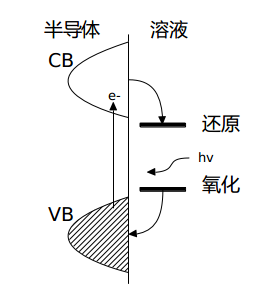
\includegraphics[scale=0.6]{figures/光催化机理图} 
\end{block}
\column{0.5\textwidth}
\begin{block}{}
半导体有一个禁带能宽,当照射进来的光的能量超过禁带能宽时,就会把价带(VB)的电子激发并进入导带(CB)。这样在价带会形成空穴,而在导带会形成额外的电子,通常这些空穴—电子对是成对出现的。
\end{block}
\end{columns}
\end{frame}


\begin{frame}
\frametitle{Fujishima的开创性工作}
\begin{block}{}
\centering
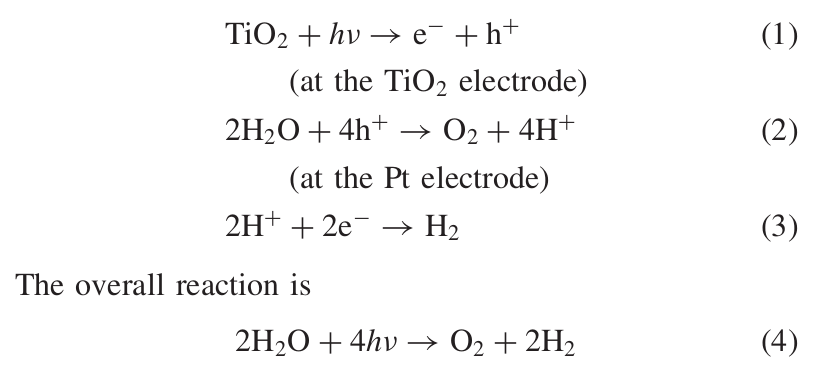
\includegraphics[scale=0.3]{figures/光分解水化学反应式} 
\end{block}
\begin{block}{}
其中\chemfig{\mathbf{TiO_2}}是光电阳极释放电子,Pt是光电阴极在这里释放氧气。整个反应就是水的分解反应。这个光化学电池量子效率是非常低下的,大约为0.1。
\end{block}
\end{frame}

\subsection{纳米三氧化二铋的性质}
\begin{frame}
\frametitle{纳米三氧化二铋的性质}
\begin{columns}
\column{0.7\textwidth}
\begin{block}{}
\centering
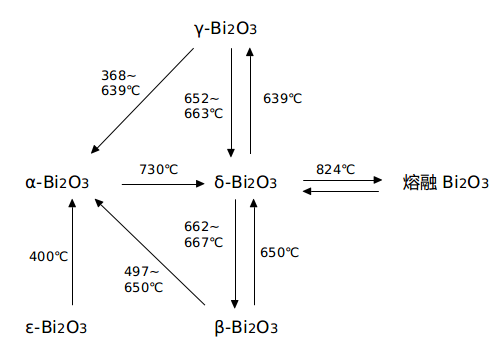
\includegraphics[width=\linewidth]{figures/Bi2O3转变温度} 
\end{block}
\column{0.3\textwidth}
\begin{block}{}
其中α-\chemfig{\mathbf{Bi_2O_3}}是室温下最稳定的构型,α-\chemfig{\mathbf{Bi_2O_3}}的禁带能宽为2.85 eV,对大部分可见光都应有吸收和响应。
\end{block}
\end{columns}
\end{frame}

\begin{frame}
\frametitle{三氧化二铋的缺陷}
\begin{columns}
\column{0.5\textwidth}
\begin{block}{光生电子—空穴复合率过高}
其中光生电子—空穴对复合率过高主要是通过调整光催化材料的晶体结构,比如通过提高结晶度加速光生电子—空穴对的分离,或者更细小的纳米粒子也会促进光生电子和空穴的分离。
\end{block}
\column{0.5\textwidth}
\begin{block}{结构不太稳定}
而\chemfig{\mathbf{Bi_2O_3}}结构不太稳定的问题Lei Huang做了专门的探讨。α-\chemfig{\mathbf{Bi_2O_3}}在空气中存放6个月就会部分转变成\chemfig{\mathbf{Bi_2O_2CO_3}},这一过程在水溶液中会进一步加速进行,这可能是因为空气中的\chemfig{\mathbf{CO_2}}溶于水生成\chemfig{\mathbf{HCO^{3-}}}和α-\chemfig{\mathbf{Bi_2O_3}}发生了反应。
\end{block}
\end{columns}
\end{frame}


\subsection{掺杂改性理论}
\begin{frame}
\frametitle{掺杂改性理论}
\begin{block}{}
金属掺杂目前认为主要有两点:一是引入杂化轨道从而降低禁带能宽,二是过渡金属可能捕捉电子从而降低光生电子─空穴复合率。非金属掺杂理论目前还没有形成一致的见解,有以下三种说法:一是非金属掺杂同样降低了禁带能宽,二是引入不纯的能级,三是比如N掺杂引入了额外的氧空位。
\end{block}
\end{frame}

\subsubsection{稀土元素掺杂}
\begin{frame}
\frametitle{稀土元素掺杂}
\begin{block}{}
比如 Krishna Reddy 的工作显示将Sm掺杂到氧化铋中,在 450-600 nm 范围内出现了明显的红移现象,这可以解释为 Sm 掺入\chemfig{\mathbf{Bi_2O_3}}晶格中形成\chemfig{\mathbf{Sm-O-Bi}}杂化轨道,从而降低了\chemfig{\mathbf{Bi_2O_3}}的禁带能宽。其中掺杂质量比 1\%的样品降解甲基蓝效率最高,三个小时内将甲基蓝完全降解,这应该得益于样品对可见光区域响应增强。
\end{block}
\end{frame}

\subsubsection{其他元素掺杂}
\begin{frame}
\frametitle{其他元素掺杂}
\begin{block}{}
Wu xiao hong 则是用溶胶凝胶法制备了 Fe 掺杂的氧化铋薄膜,Fe 掺杂并没有让氧化铋对光的吸收有明显的差异,不过 Fe 掺杂让氧化铋降解罗丹明 B 的效率有了显着的提升,在摩尔比约为 3/100 的时候 15 min 降解率就达到了 98\%,比纯的氧化铋效率提高了 40\%。作者解释到这应该得益于纳米材料粒径变小和光生电子-空穴复合率降低。
\end{block}
\end{frame}

\subsection{异质结改性理论}
\begin{frame}
\frametitle{异质结改性理论}
\begin{block}{}
构建物质的异质结有时能够达到比单独两个物质更好的光催化活性。这是因为两个不同物质的CB(导带)和VB(价带)能级差异,使得光生电子能够在两个物质融合的晶格面发生小能级的跃迁,从而将一次大的能级跃迁变成几次能级更小的跃迁。而多个能级晶格面的存在还提高了光生电子-空穴对分离率。此外不同的晶型物质混杂成型可能会降低纳米粒子的尺寸,从而达到提高比表面积,增强光催化活性的目的。
\end{block}
\end{frame}

\begin{frame}
\frametitle{和铋基光催化材料构建异质结}
\begin{block}{}
Ming Sheng Gui 等将\chemfig{\mathbf{Bi_2O_3}}和\chemfig{\mathbf{Bi_2WO_6}}一起构建异质结,在\chemfig{\mathbf{Bi_2WO_6}}基底上逐渐增加纳米\chemfig{\mathbf{Bi_2O_3}}的负载量,到达
质量比 3\%的时候光催化性能最好,比单独的\chemfig{\mathbf{Bi_2O_3}}或者\chemfig{\mathbf{Bi_2WO_6}}都要好 。作者说这主要是因为催化材料对光的吸收增强和光生电子-空穴复合率降低。值得一提的是这种异质结光催化材料的稳定性非常好,重复使用 4 次之后活性没有明显的降低。
\end{block}
\end{frame}

\begin{frame}
\frametitle{和金属构建异质结}
\begin{block}{}
和纯金属构建异质结也有报道,比如 Zhong Jun Bo 等将 Ag 负载到\chemfig{\mathbf{Bi_2O_3}}构建
异质结从而得到结论负载质量比为 0.5\%的时候光催化性能最好。从 SPS 图谱分析,银负载能够有效分离光生电子-空穴对,从而达到提高光催化效率的目的。
\end{block}
\end{frame}

\begin{frame}
\frametitle{和其他金属氧化物构建异质结}
\begin{block}{}
Abdul Hameed 构建的\chemfig{\mathbf{NiO/Bi_2O_3}}显示这种异质结催化材料的光催化活性要比单独各自纯物质的活性明显高很多。除了常见的异质结解释理论外,作者还提到这两种晶型的物质存在著某种作用从而让 NiO 和\chemfig{\mathbf{Bi_2O_3}}在形成异质结的时候纳米晶粒尺寸有所缩减。晶粒尺寸的缩减,比表面积的增加还会继续提高光催化活性。
\end{block}
\end{frame}


\section{掺杂改性的研究}
\subsection{镨掺杂}
\begin{frame}
\frametitle{镨掺杂三氧化二铋的研究}
\begin{block}{实验制备方法}
实验采用柠檬酸盐溶胶凝胶法制备镨掺杂的三氧化二铋。在250mL烧杯里加入100 mL去离子水,然后加入9.0108 g的柠檬酸。搅拌,待全部溶解之后加入20.8 g五水硝酸铋。然后按照镨与铋的原子摩尔掺杂比依次加入六水硝酸镨。搅拌两个小时后,进入115度烘箱,直到水分完全蒸发,形成干凝胶。然后放入马弗炉,300度保温一个小时,500度保温两个小时即得样品。
\end{block}
\end{frame}

\begin{frame}
\frametitle{镨掺杂系列XRD图谱}
\begin{columns}
\column{0.5\textwidth}
\begin{block}{}
\centering
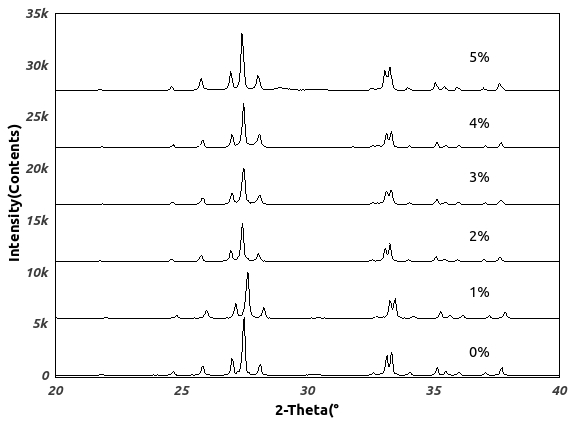
\includegraphics[width=\linewidth]{figures/镨掺杂XRD.jpg} 
\end{block}
\column{0.5\textwidth}
\begin{block}{}
从图中可以看出各个谱线并没有明显的差异。分析显示各个样品和铋赭石晶型十分吻合,其中角度 27.437(120)处为 α-\chemfig{\mathbf{Bi_2O_3}}的特征衍射峰。并没有检测到镨元素或者氧化铋的其他晶相。这表明镨元素的掺杂并没有改变三氧化二铋原有的晶体结构。
\end{block}
\end{columns}
\end{frame}

\begin{frame}
\frametitle{镨掺杂系列晶粒尺寸}
\begin{columns}
\column{0.5\textwidth}
\begin{block}{}
\centering
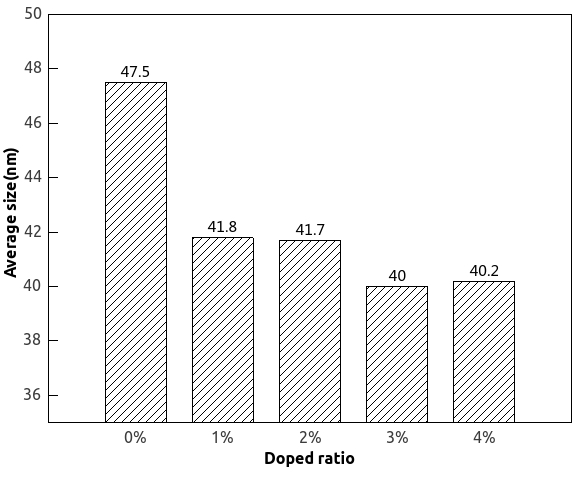
\includegraphics[width=\linewidth]{figures/镨掺杂粒径大小.jpg} 
\end{block}
\column{0.5\textwidth}
\begin{block}{}
从图中可以看出该方法制得的催化剂总的平均晶粒尺寸大小在 40-48 纳米之间。而镨的掺杂刚开始能够稍微减少晶粒尺寸,后面随着掺杂量的增加这种减少尺寸的效应就很微弱了。这可能是因为镨的掺杂抑制了氧化铋之间的团聚现象。
\end{block}
\end{columns}
\end{frame}


\begin{frame}
\frametitle{镨掺杂系列Uv-Vis图谱}
\begin{block}{}
\centering
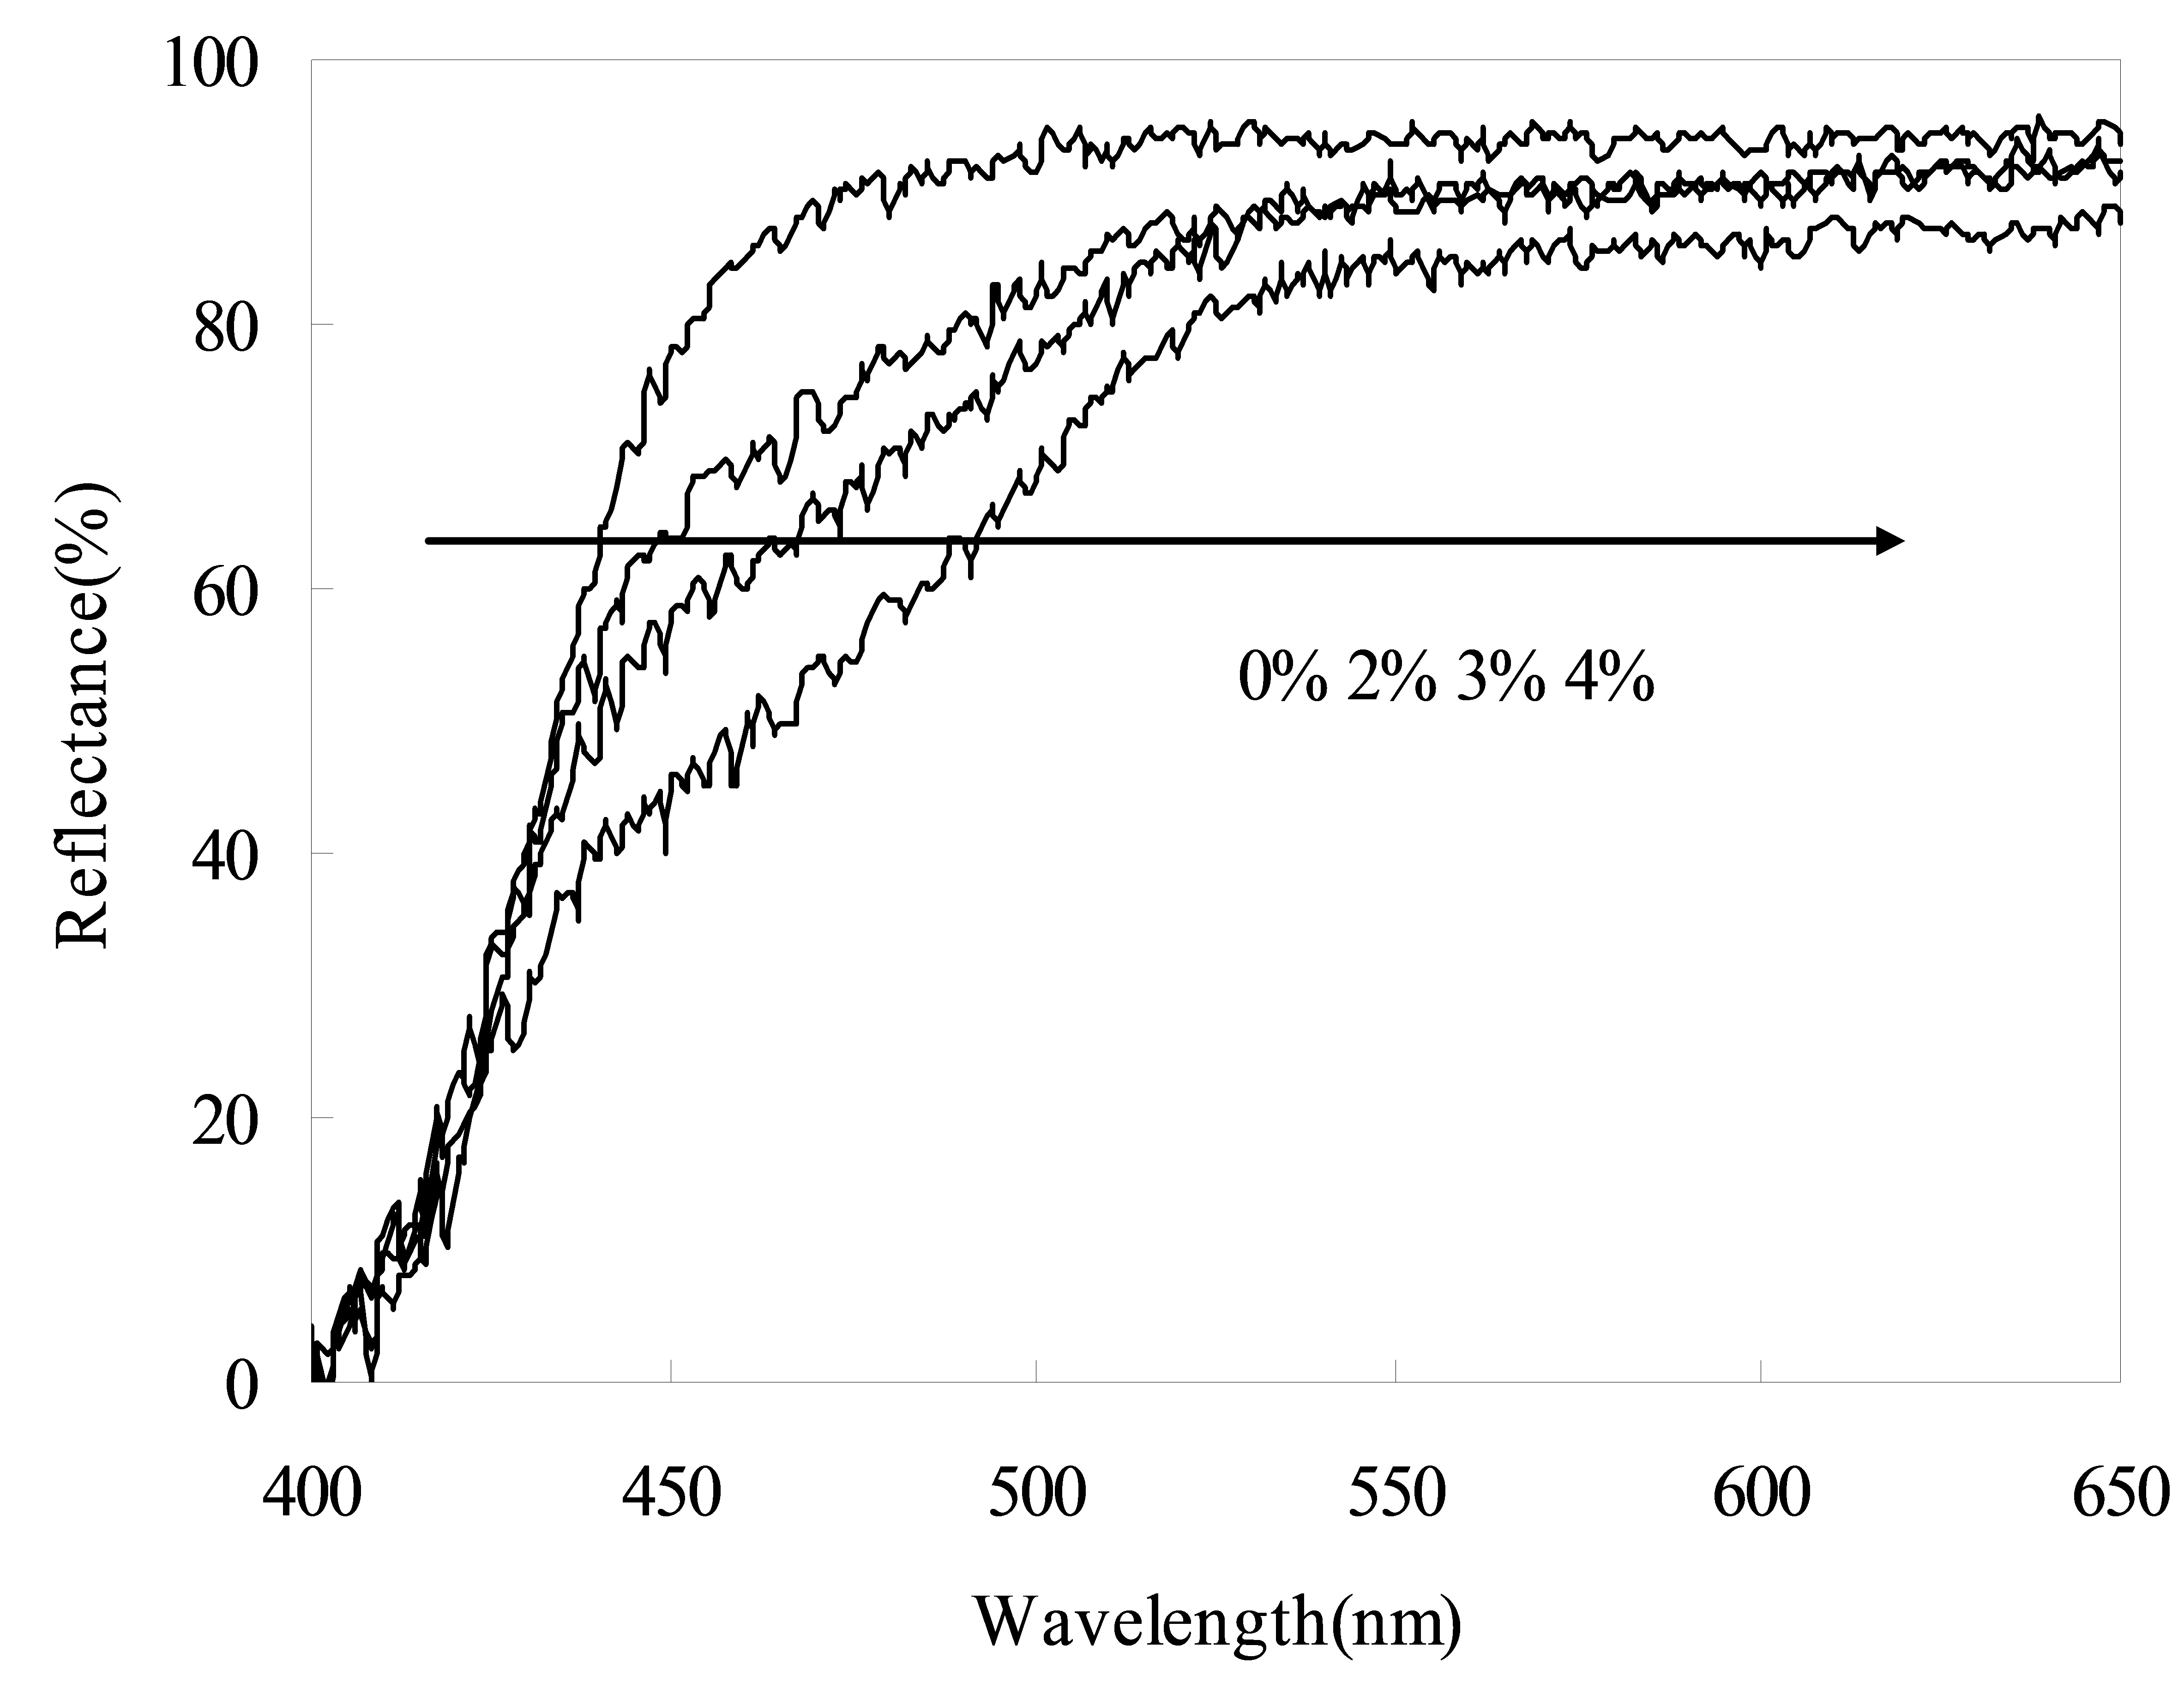
\includegraphics[width=0.8\linewidth]{figures/镨掺杂UV.jpg} 
\end{block}
\end{frame}

\begin{frame}
\frametitle{镨掺杂系列Uv-Vis图谱分析}
\begin{block}{}
从图中可以明显看出谱线下移现象。在波长 400-550 nm 范围内这种下移现象最为明显,波长 550-700 nm 范围内有轻微的下移。当掺杂量达到 2\%的时候,有一个跳跃性的下移现象,然后后面随着掺杂量的
增加,谱线继续下移。随着掺杂量的增加,对可见光的响应变好,说明掺杂在一定程度上混杂了 CBM(最低导带)轨道,从而电子从 VBM(最高价带)跃迁到 CBM 的所需能量降低,从而实现了某些低能光子的吸收
\end{block}
\end{frame}

\begin{frame}
\frametitle{镨掺杂系列SPS图谱}
\begin{block}{}
\centering
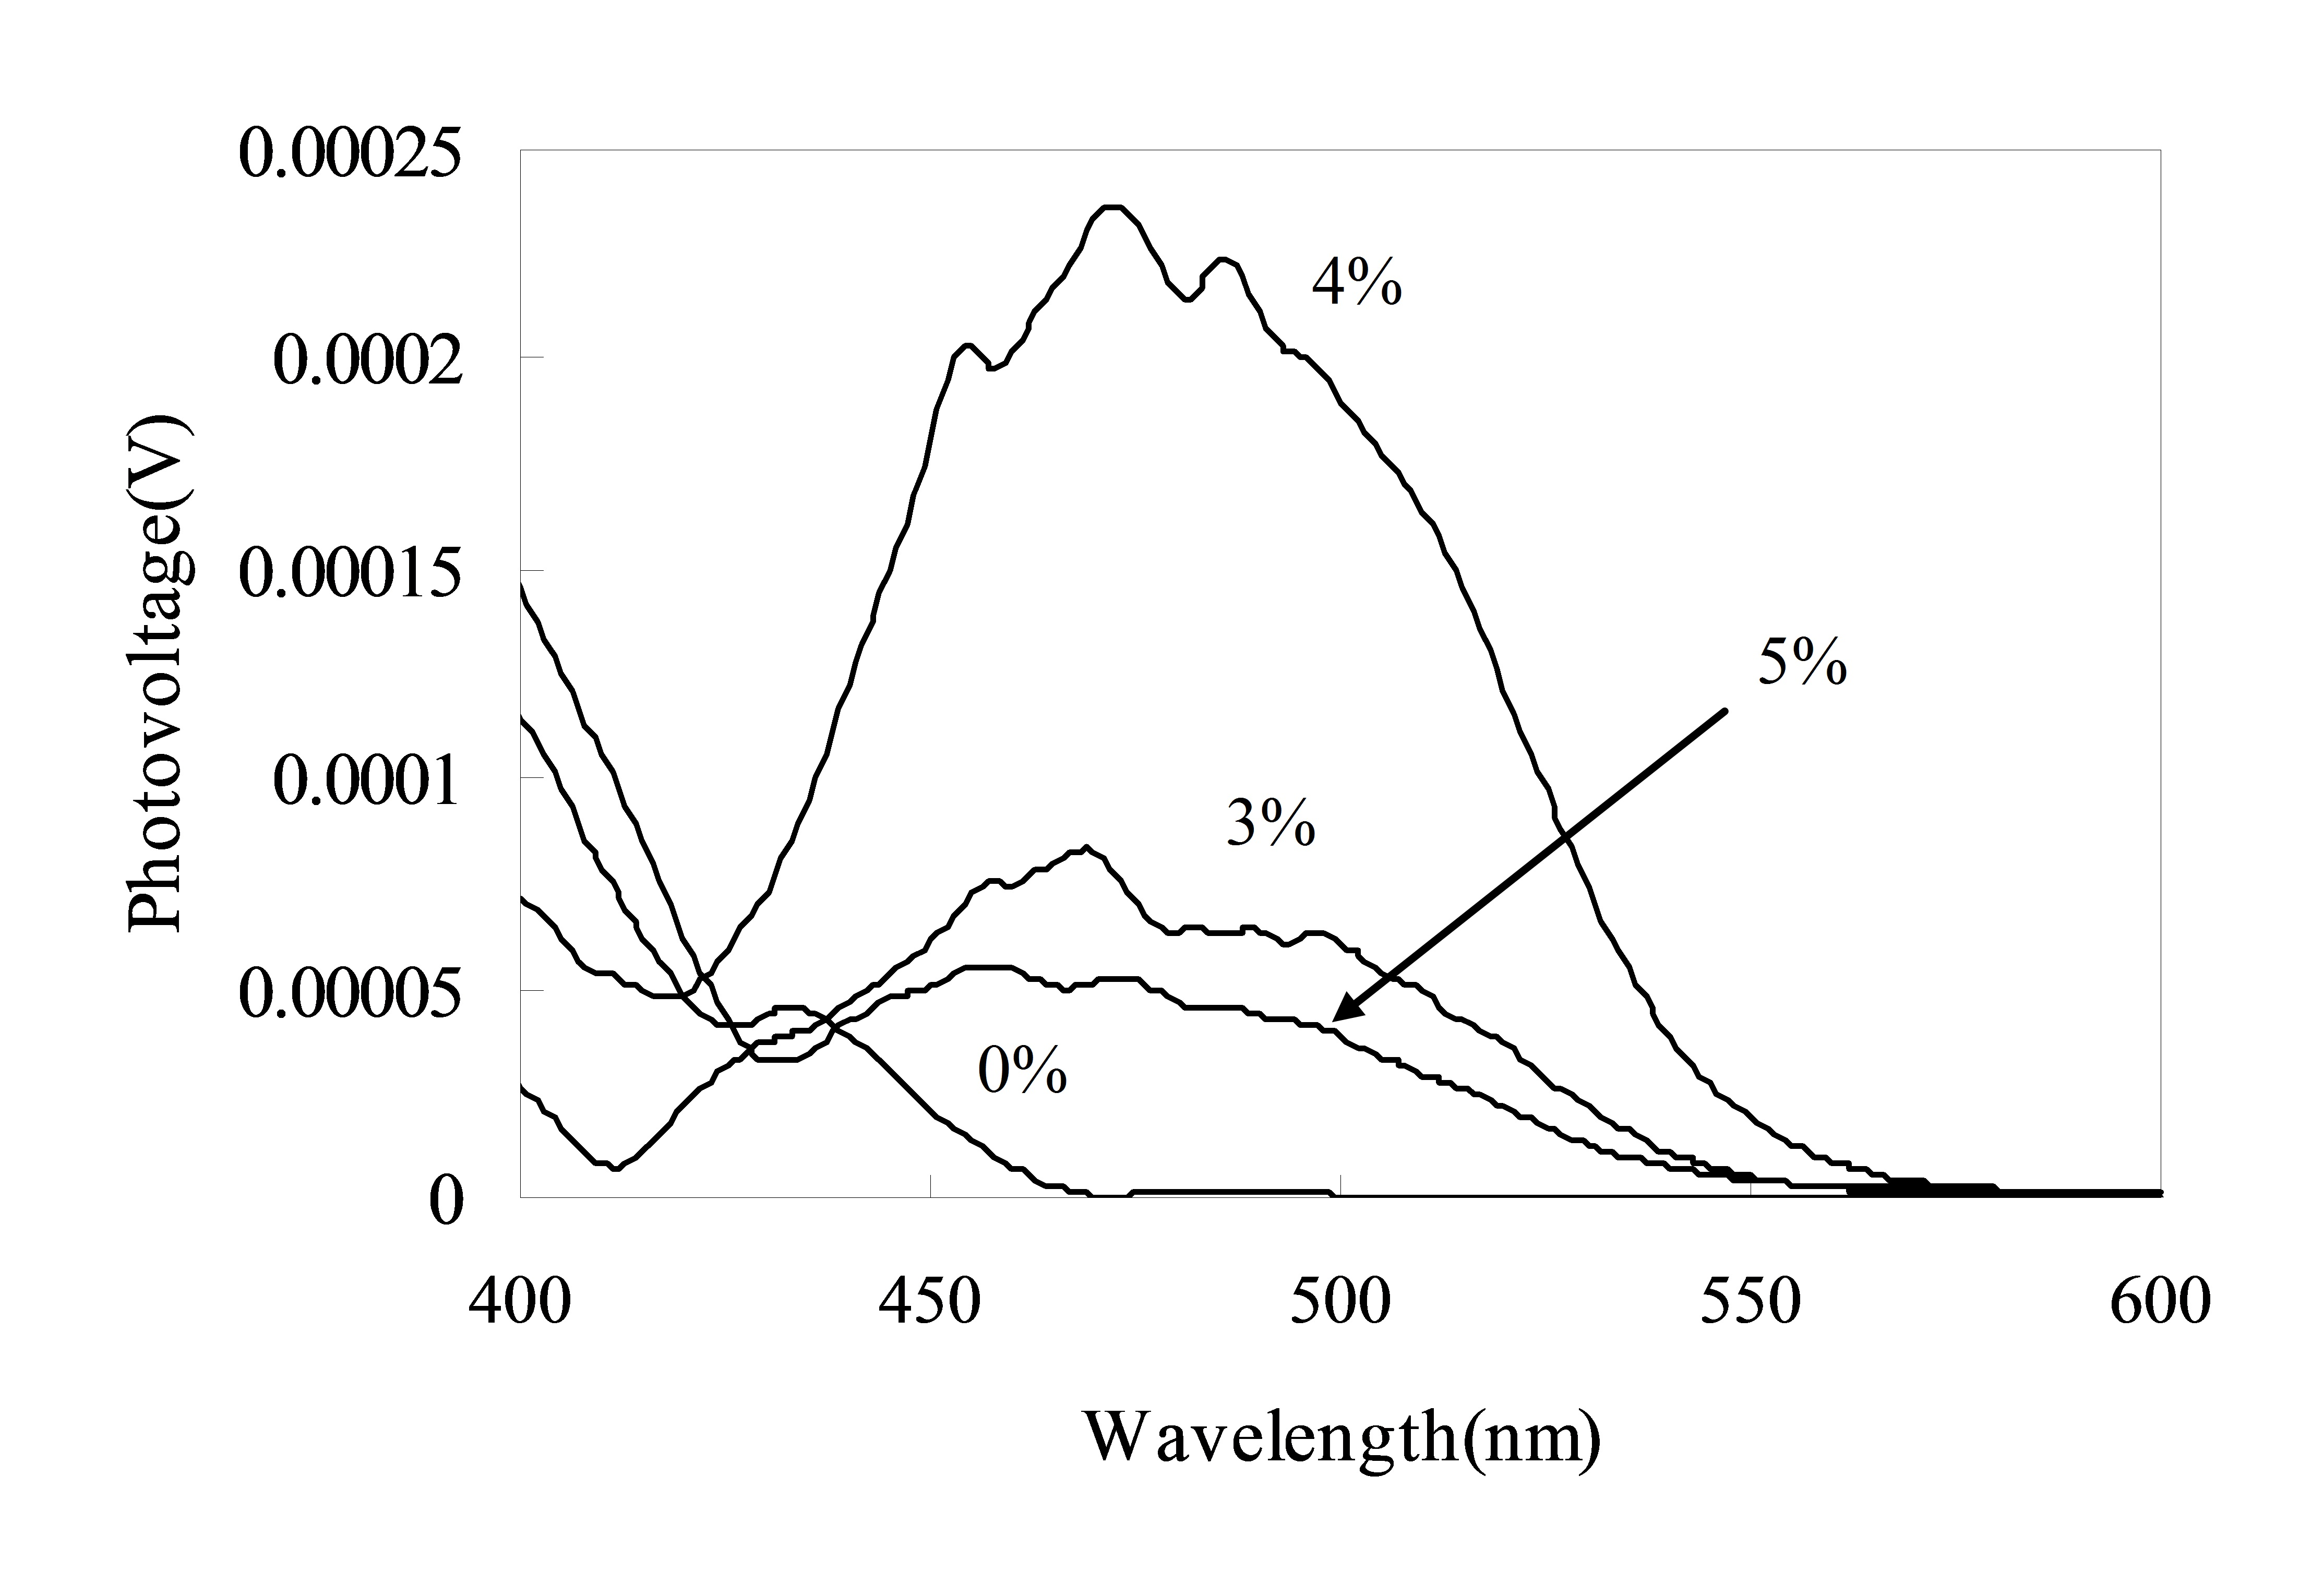
\includegraphics[width=0.8\textwidth]{figures/镨掺杂SPS.jpg} 
\end{block}
\end{frame}

\begin{frame}
\frametitle{镨掺杂系列SPS图谱分析}
\begin{block}{}
从图中可以看出0\%掺杂量的纯氧化铋在低能响应区信号弱的主要原因就是光生载流子生成的数量不够。然后通过前面XRD晶粒尺寸的分析大致知道后面几个掺杂量的催化剂的晶粒尺寸大小大致差不多的,
所以 4\%在450-550 纳米范围内光电信号的加强的合理解释就是对于可见光的响应加强。
\end{block}
\end{frame}


\begin{frame}
\frametitle{镨掺杂系列的光催化活性一}
\framesubtitle{在35W紫外杀菌灯下照射1h}
\begin{block}{}
\centering
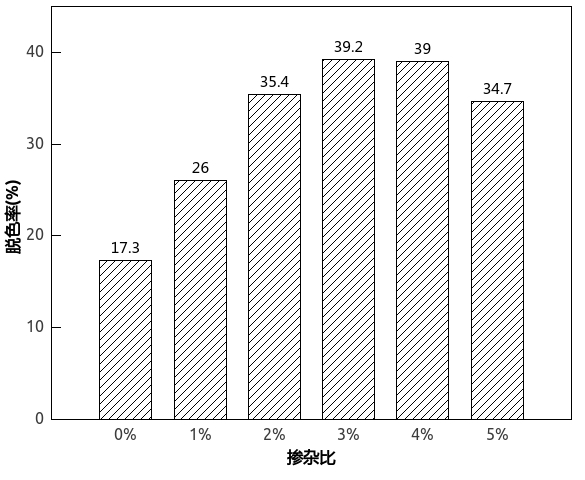
\includegraphics[scale=6]{figures/镨掺杂活性1.jpg} 
\end{block}
\end{frame}

\begin{frame}
\frametitle{镨掺杂系列的光催化活性二}
\framesubtitle{在350W氙灯下照射4h}
\begin{block}{}
\centering
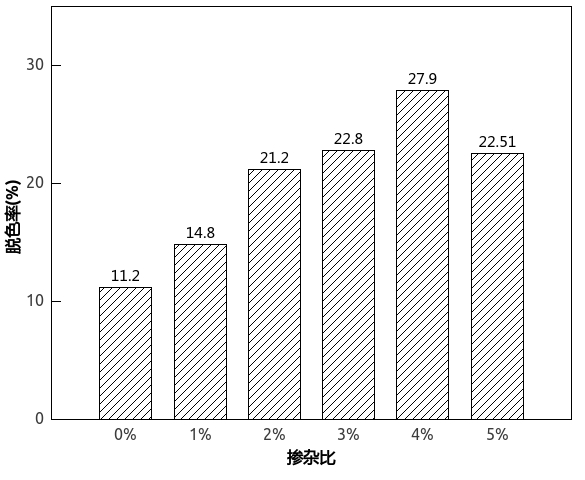
\includegraphics[scale=6]{figures/镨掺杂活性2.jpg} 
\end{block}
\end{frame}


\subsection{钕掺杂}
\begin{frame}
\frametitle{钕掺杂系列XRD图谱}
\begin{block}{}
\centering
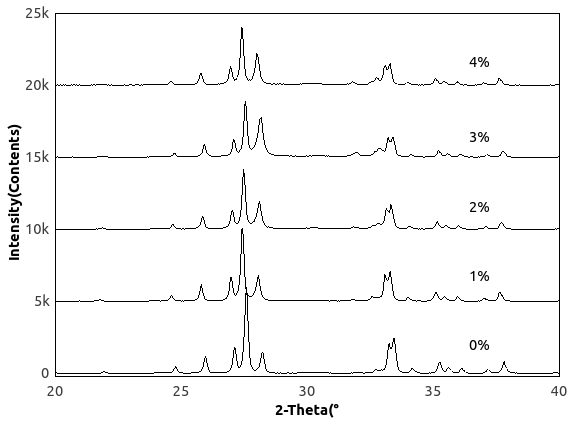
\includegraphics[scale=7]{figures/钕掺杂XRD.jpg} 
\end{block}
\end{frame}

\begin{frame}
\frametitle{钕掺杂系列晶粒尺寸}
\begin{columns}
\column{0.5\textwidth}
\begin{block}{}
\centering
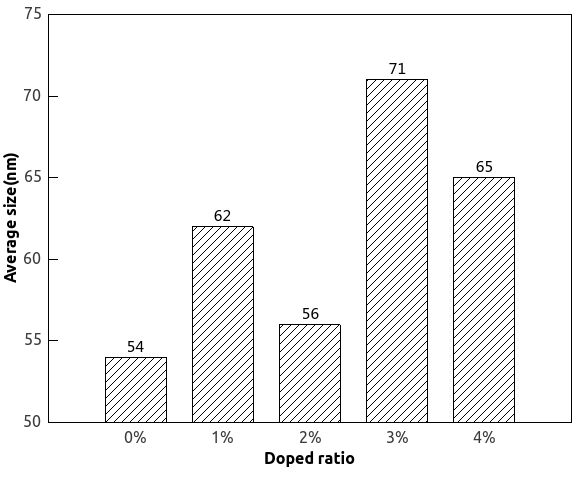
\includegraphics[width=\linewidth]{figures/钕掺杂粒径大小.jpg} 
\end{block}
\column{0.5\textwidth}
\begin{block}{}
从图中可以看出该方法制得的催化剂总的平均晶粒尺寸大小在 55-70 纳米之间。钕的掺杂比超过 2\%之后会很大的增大了催化剂的晶粒大小,可能是氧化钕的存在促进了氧化铋晶粒的聚合。这并不利于光催化反应的。
\end{block}
\end{columns}
\end{frame}

\begin{frame}
\frametitle{钕掺杂系列Uv-Vis图谱}
\begin{block}{}
\centering
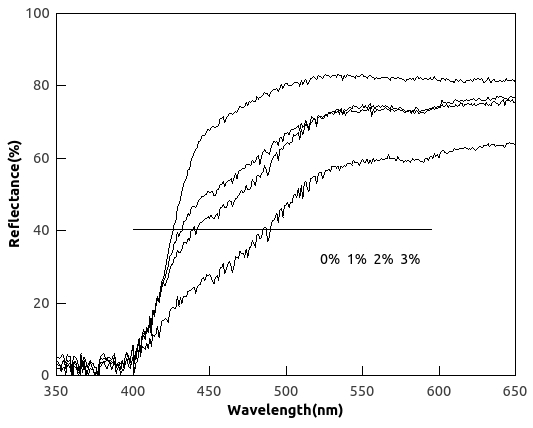
\includegraphics[scale=7]{figures/钕掺杂UV.jpg} 
\end{block}
\end{frame}


\begin{frame}
\frametitle{钕掺杂系列SPS图谱}
\begin{block}{}
\centering
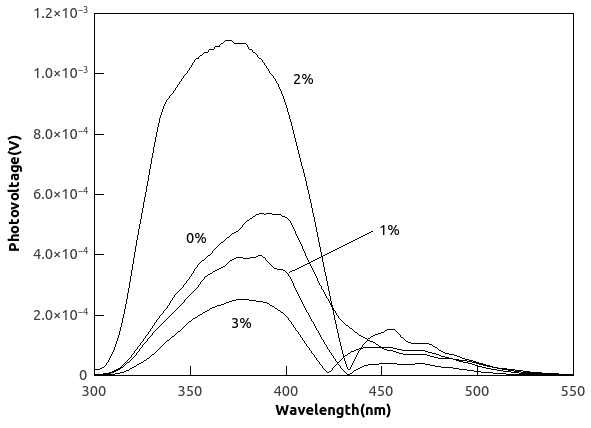
\includegraphics[scale=7]{figures/钕掺杂SPS.jpg} 
\end{block}
\end{frame}


\begin{frame}
\frametitle{钕掺杂系列的光催化活性}
\framesubtitle{在350W氙灯下照射4h}
\begin{block}{}
\centering
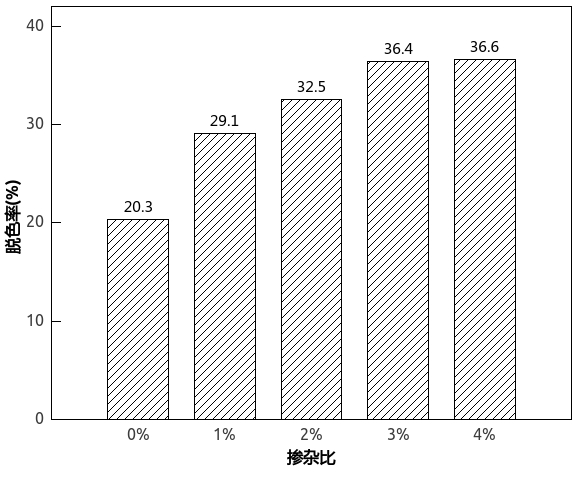
\includegraphics[scale=6]{figures/钕掺杂活性.jpg} 
\end{block}
\end{frame}

\subsection{掺杂改性总结}
\begin{frame}
\frametitle{掺杂改性总结}
\begin{block}{}
\begin{itemize}
\item<1> 掺杂Pr3+后Bi2O3晶粒尺寸变小,比表面增加,对可见光的响应增强,4\%掺杂量样品在可见光区表面光电压响应最强,在模拟太阳光和紫外光照射下掺杂样品对甲基橙光催化活性得到显著提高,其中4\%Pr掺杂样品具有最好的可见光催化活性。%\pause
\item<2> 掺杂Nd3+后Bi2O3晶粒尺寸变大,对可见光的响应增强,2\%掺杂量样品在可见光区表面光电压响应最强,在模拟太阳光照射下对甲基橙光催化活性得到显著提高,其中3\%-4\%Nd掺杂样品具有最好的可见光催化活性。
\end{itemize}
\end{block}
\end{frame}

\section{异质结改性的研究}
\subsection{三氧化二铟}
\begin{frame}
\frametitle{\chemfig{\mathbf{In_2O_3/ Bi_2O_3}}光催化剂的比表面积}
\centering
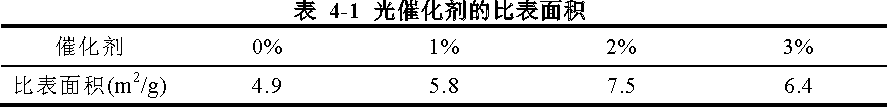
\includegraphics[width=\textwidth]{figures/三氧化二铟比表面积.pdf} 
\begin{block}{}
随\chemfig{\mathbf{In_2O_3}}负载量逐渐增加,光催化剂比表面逐渐增加,当 In/Bi 摩尔比为 2\%时,催化剂的比表面最大,进一步增加\chemfig{\mathbf{In_2O_3}}负载量比表面下降。\chemfig{\mathbf{In_2O_3}}的负载量较低时比表面较小;而\chemfig{\mathbf{In_2O_3}}的负载量过高时,大量的\chemfig{\mathbf{In_2O_3}}在原有表面重复堆积,堵塞载体孔道,使比表面减少。
\end{block}
\end{frame}

\begin{frame}
\frametitle{\chemfig{\mathbf{In_2O_3/ Bi_2O_3}}光催化剂的XRD图谱}
\begin{block}{}
\centering
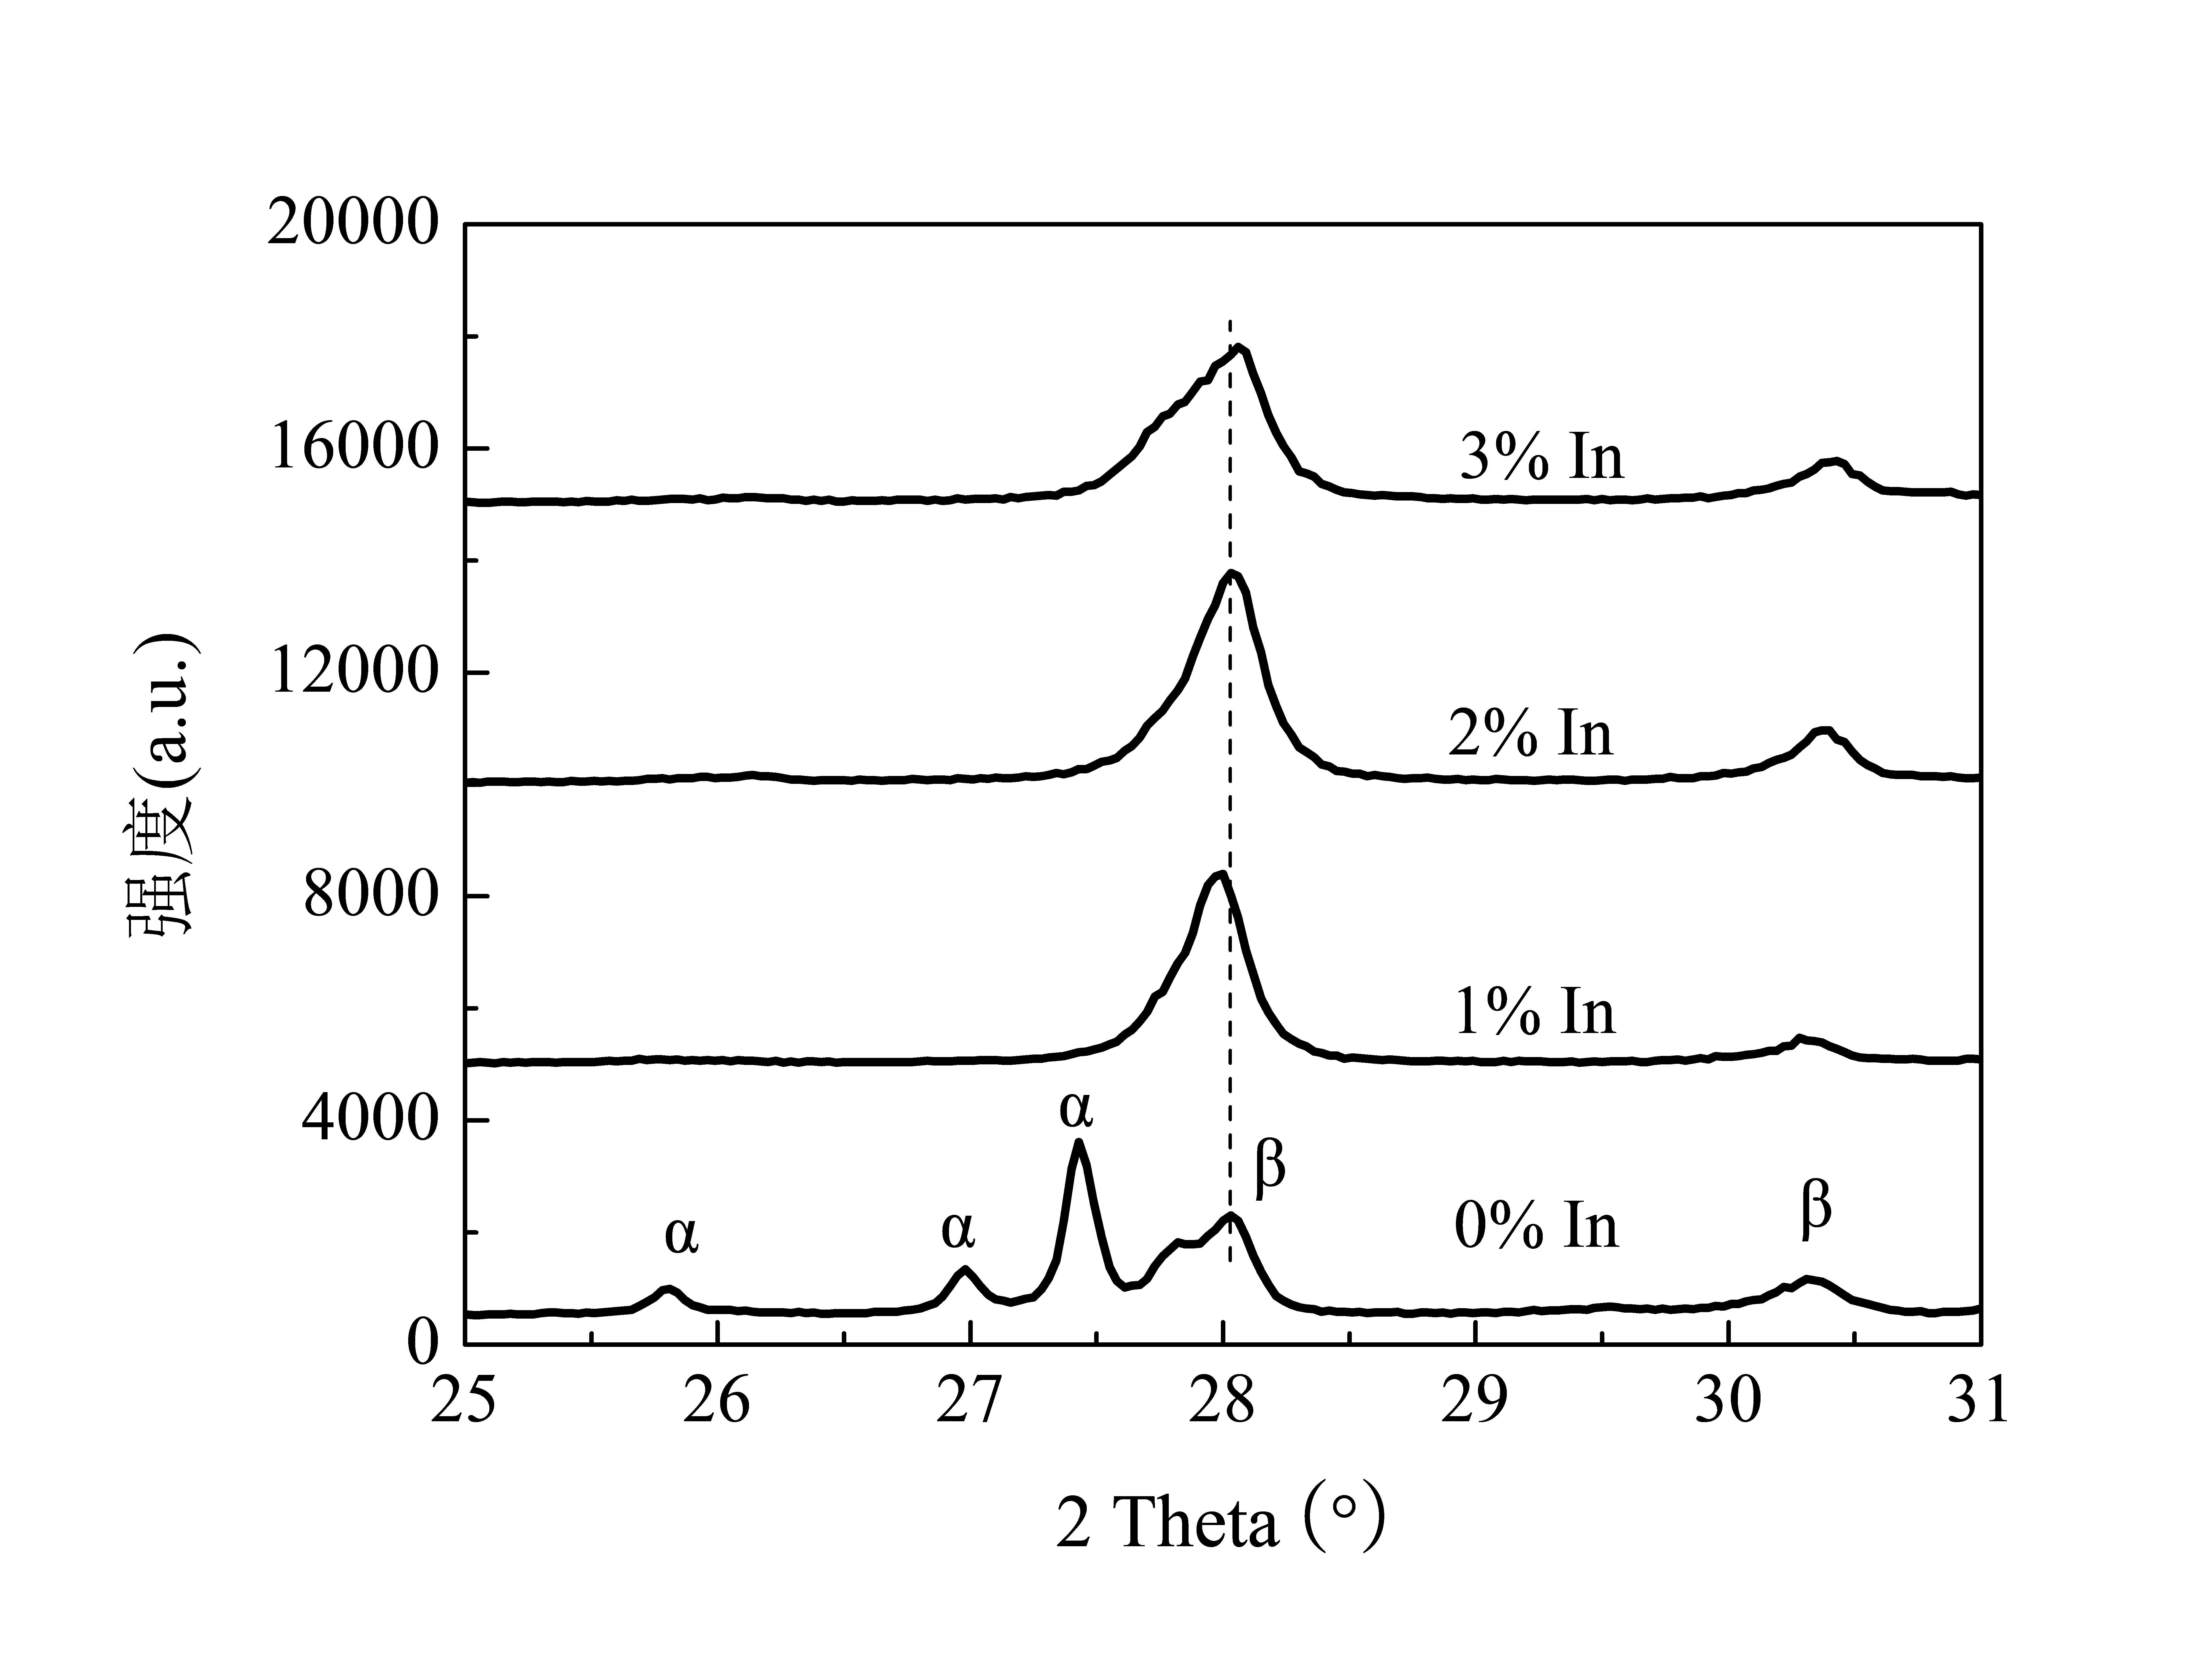
\includegraphics[width=0.85\textwidth]{figures/三氧化二铟XRD} 
\end{block}
\end{frame}

\begin{frame}
\frametitle{\chemfig{\mathbf{In_2O_3/ Bi_2O_3}}光催化剂的XRD图谱分析}
\begin{block}{}
27.45°是 α-\chemfig{\mathbf{Bi_2O_3}}的特征衍射峰;28.0°是 β-\chemfig{\mathbf{Bi_2O_3}}的特征衍射峰。但是值得注意的是对于负载型光催化剂而言,只检测到了 β-\chemfig{\mathbf{Bi_2O_3}}的特征衍射峰。同时β-\chemfig{\mathbf{Bi_2O_3}}衍射峰没有发生明显的偏移,说明\chemfig{\mathbf{In^{3+}}}有进入\chemfig{\mathbf{Bi_2O_3}}晶格替代\chemfig{\mathbf{Bi^{3+}}} 。没有检测到β-\chemfig{\mathbf{Bi_2O_3}}的特征衍射峰其原因可能是在\chemfig{\mathbf{Bi_2O_3}}表面高度分散或者含量太低。
\end{block}
\end{frame}


\begin{frame}
\frametitle{\chemfig{\mathbf{In_2O_3/ Bi_2O_3}}光催化剂的UV-Vis图谱}
\begin{block}{}
\centering
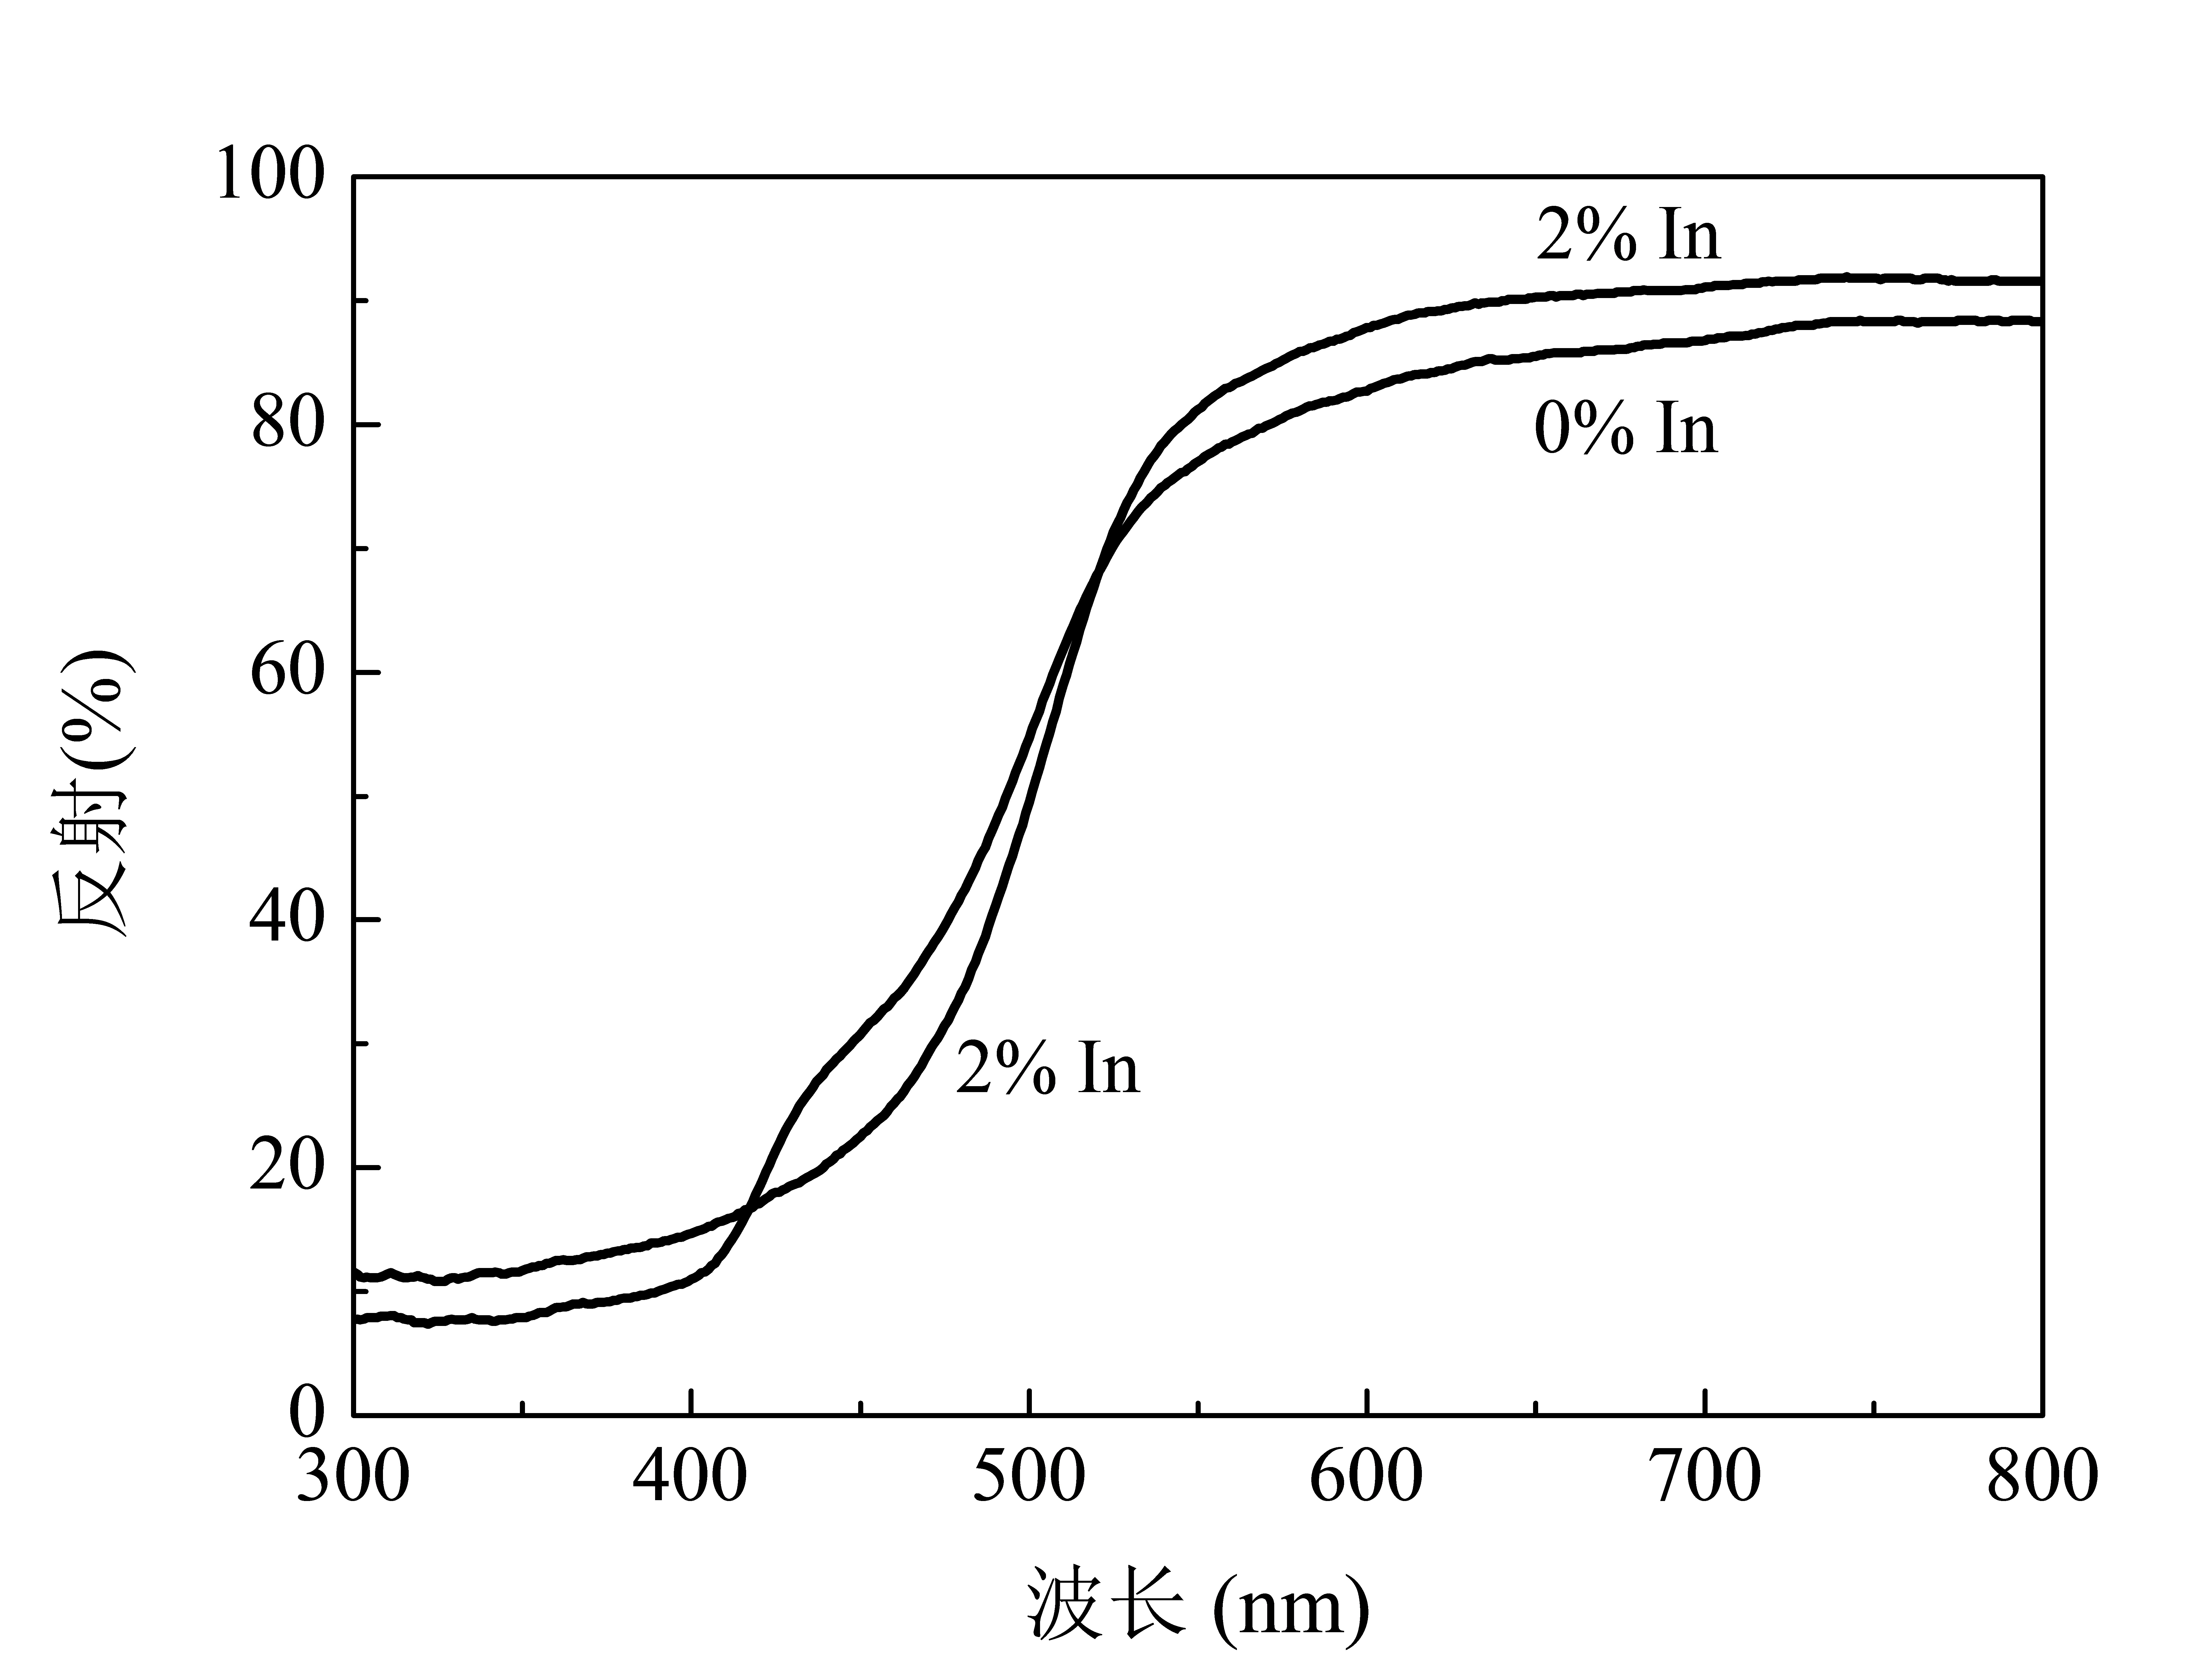
\includegraphics[width=0.8\textwidth]{figures/三氧化二铟UV.jpg} 
\end{block}
\end{frame}

\begin{frame}
\frametitle{\chemfig{\mathbf{In_2O_3/ Bi_2O_3}}光催化剂的XPS图谱}
\begin{block}{}
\centering
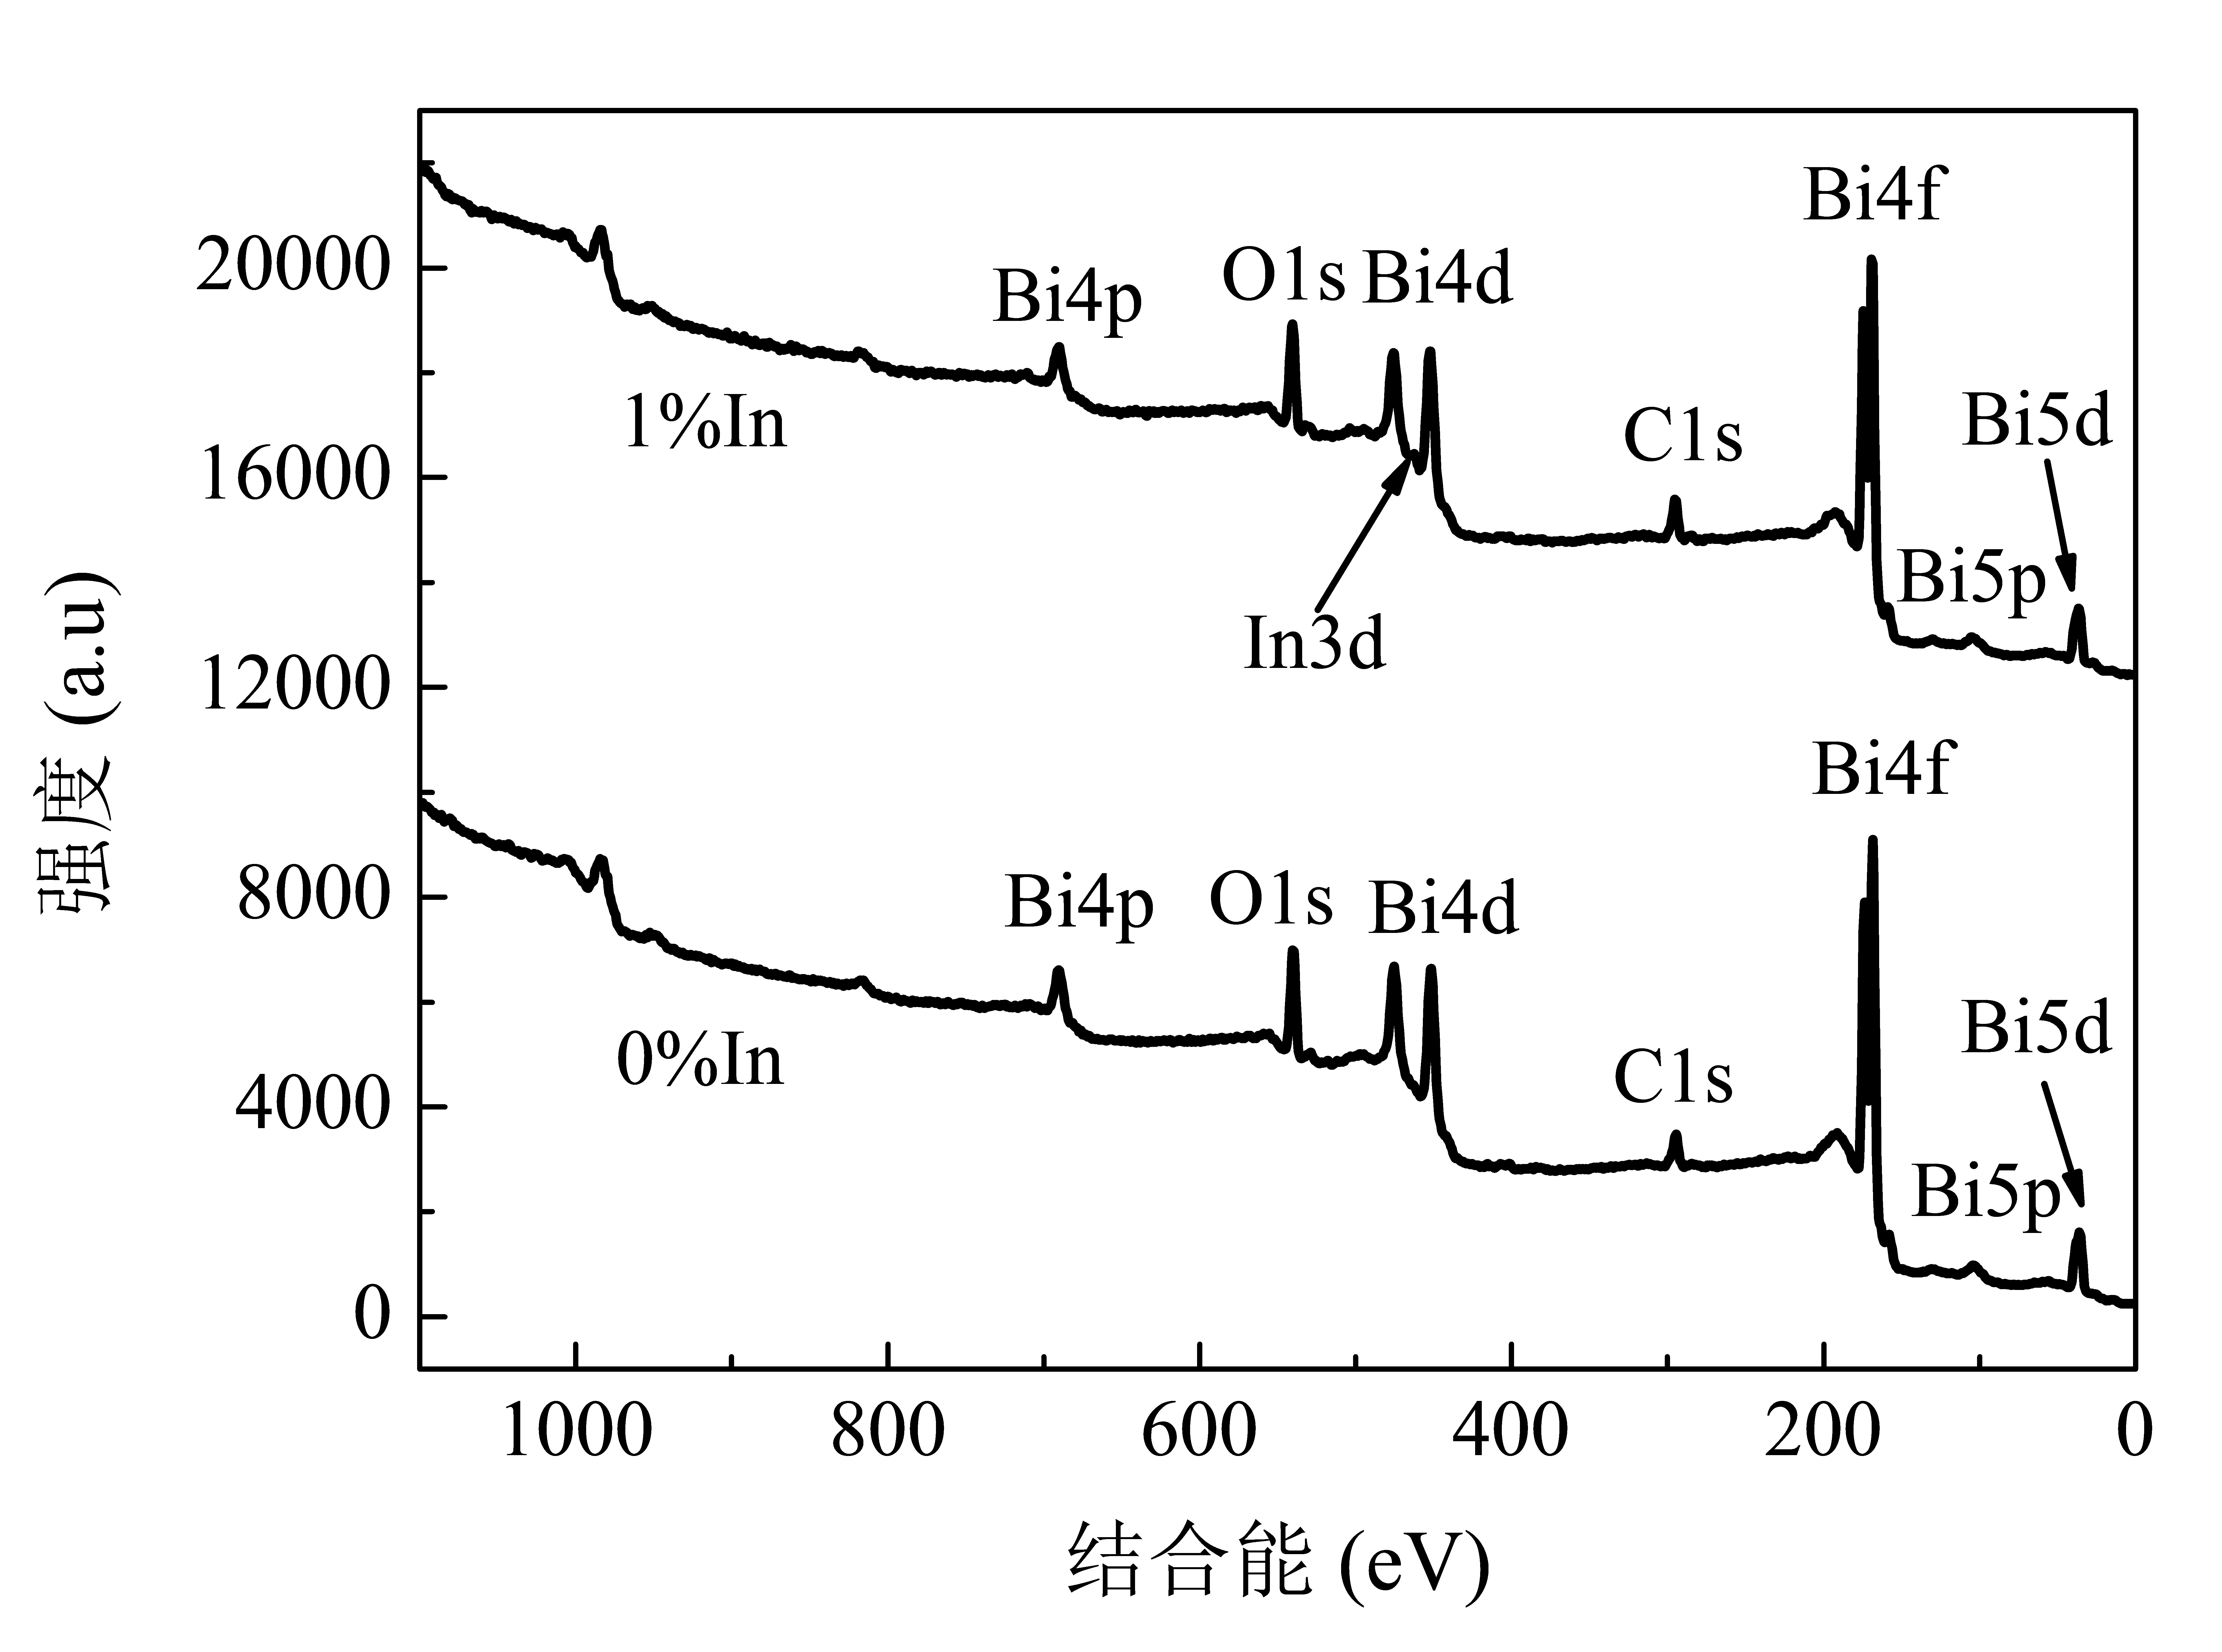
\includegraphics[width=0.8\textwidth]{figures/三氧化二铟XPS.jpg} 
\end{block}
\end{frame}

\begin{frame}
\frametitle{\chemfig{\mathbf{In_2O_3/ Bi_2O_3}}光催化剂的XPS图谱分析一}
\begin{columns}
\column{0.55\textwidth}
\begin{block}{}
\centering
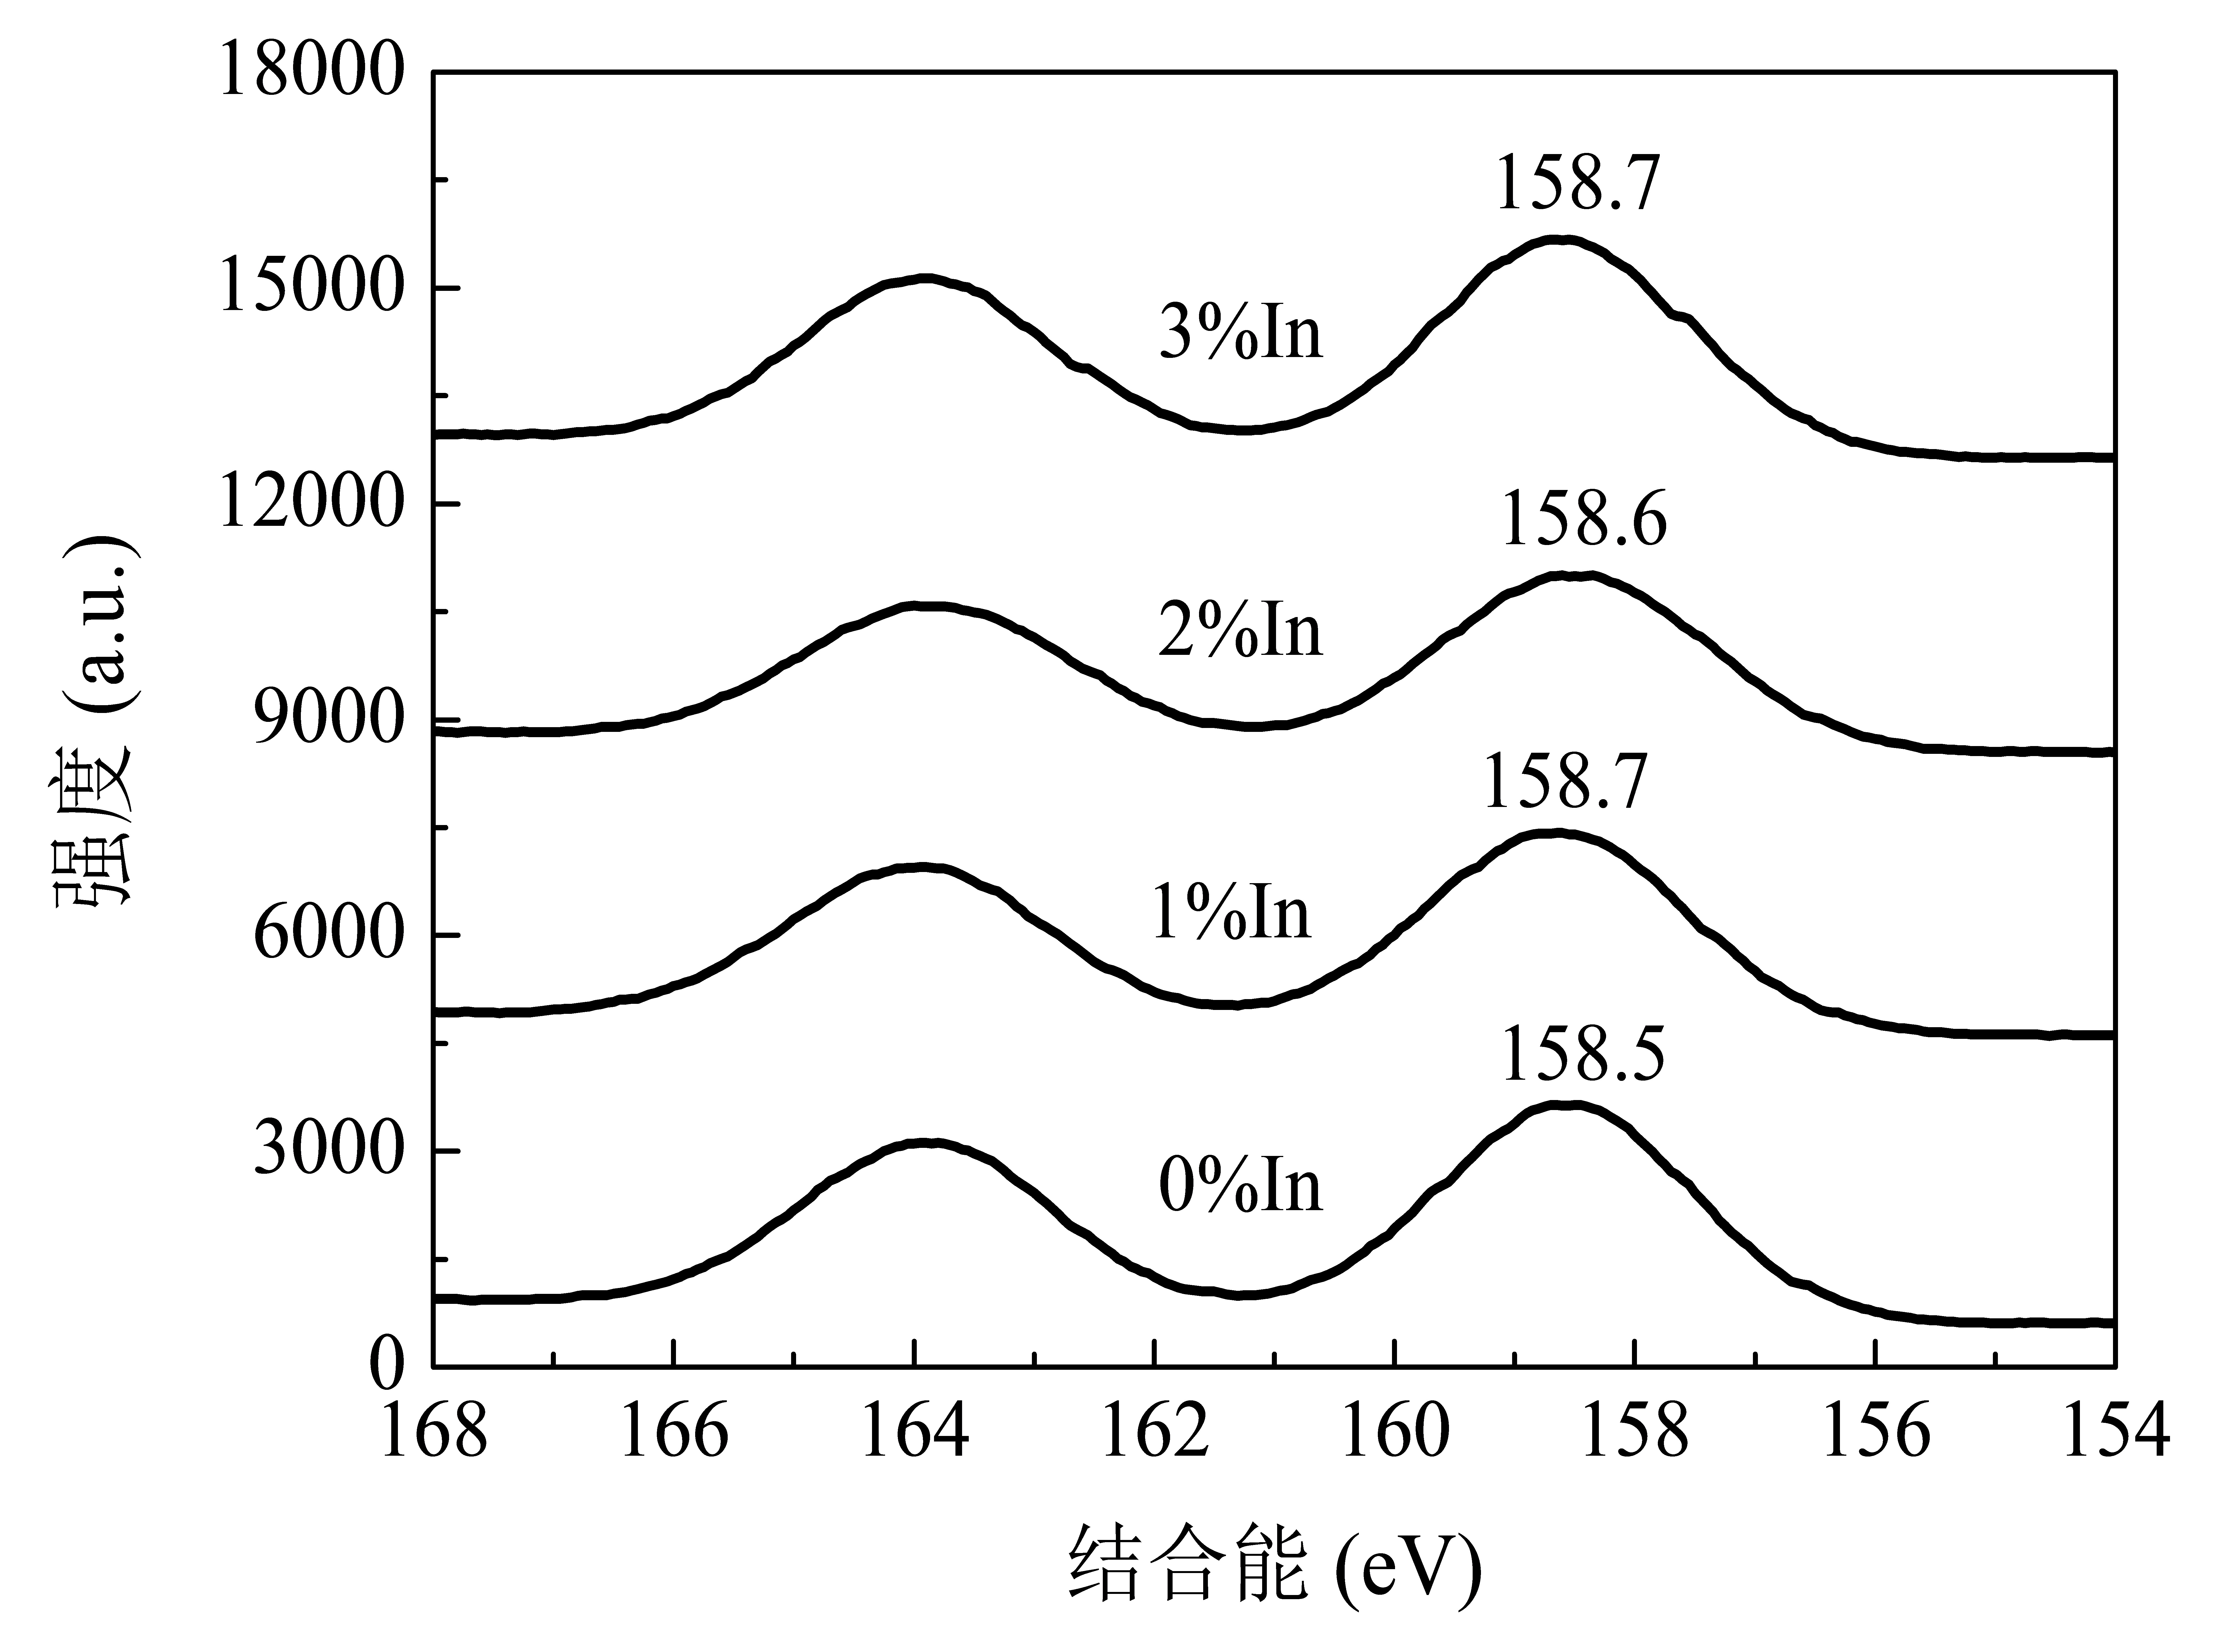
\includegraphics[width=\linewidth]{figures/三氧化二铟BI4F.jpg} 
\end{block}
\column{0.45\textwidth}
\begin{block}{Bi4f轨道分析}
对于纯\chemfig{\mathbf{Bi_2O_3}},Bi4f7/2 位于 158.5 eV,表明 Bi是3+。然而,对负载型光催化剂,Bi4f7/2向高能段偏移,这表明\chemfig{\mathbf{In_2O_3}}和\chemfig{\mathbf{Bi_2O_3}}之间发生了相互作用。
\end{block}
\end{columns}
\end{frame}

\begin{frame}
\frametitle{\chemfig{\mathbf{In_2O_3/ Bi_2O_3}}光催化剂的XPS图谱分析二}
\begin{columns}
\column{0.5\textwidth}
\begin{block}{}
\centering
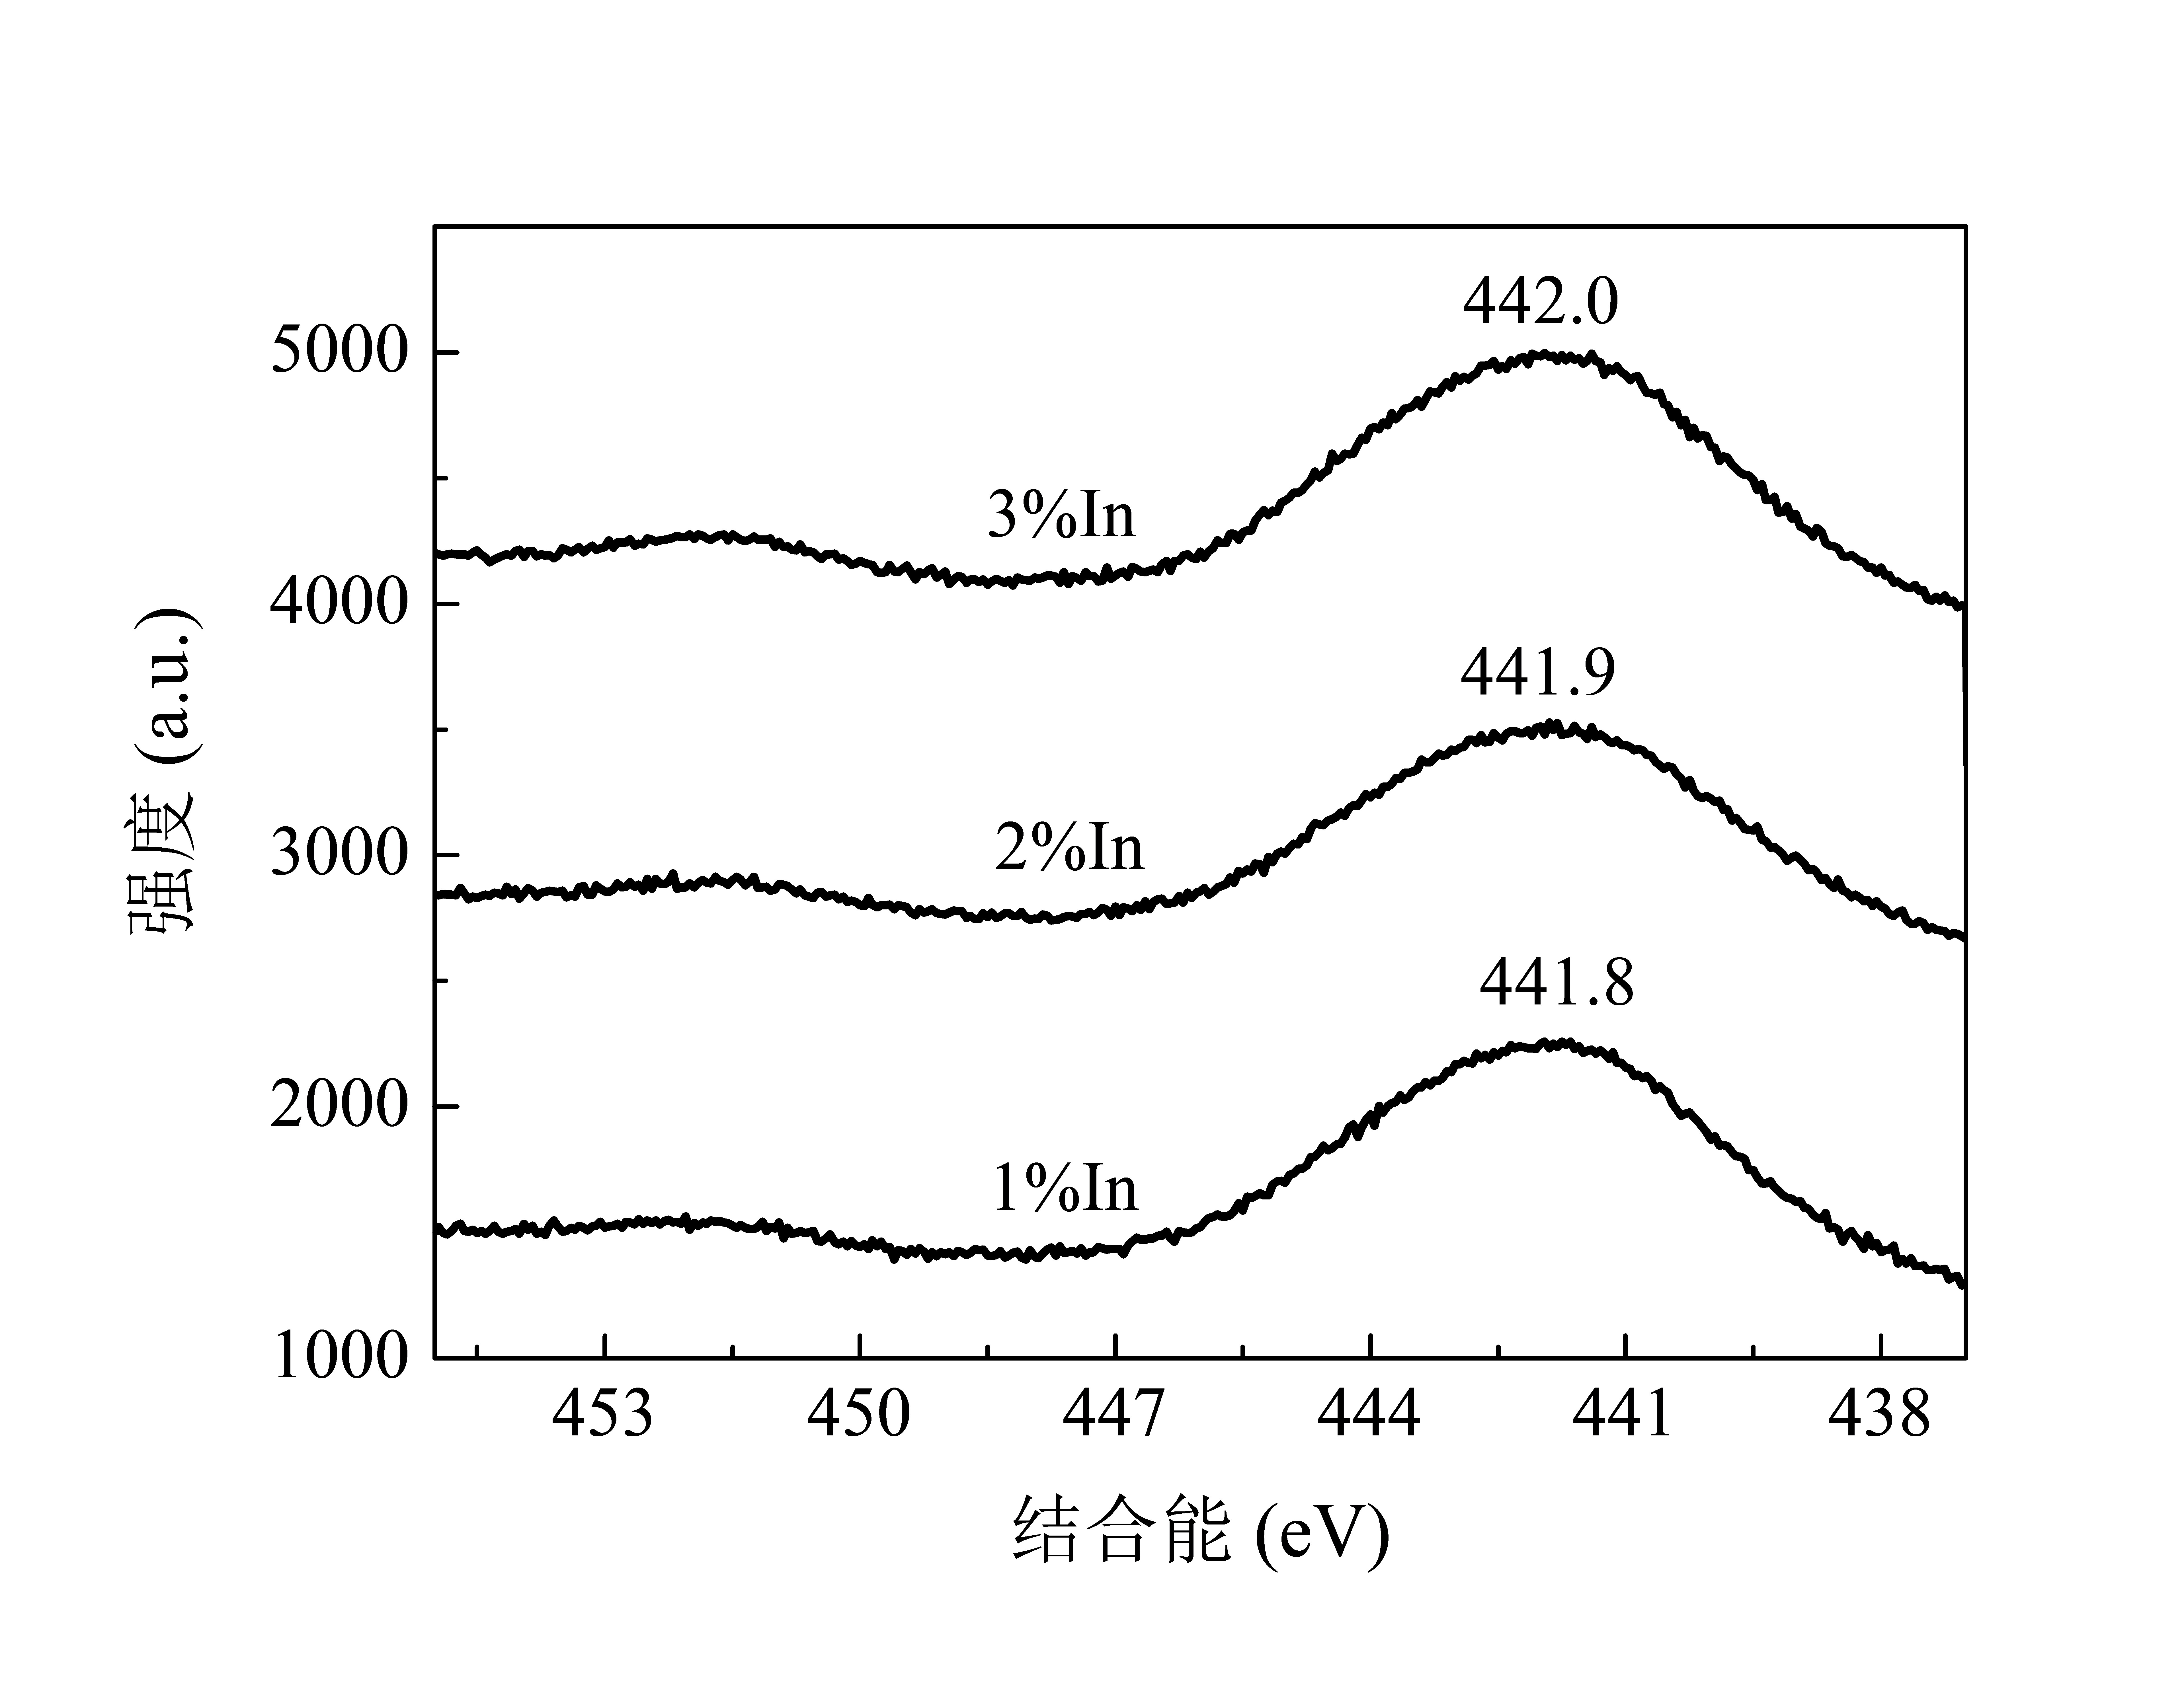
\includegraphics[width=\linewidth]{figures/三氧化二铟3D.jpg} 
\end{block}
\column{0.5\textwidth}
\begin{block}{In3d轨道分析}
文献报道对于\chemfig{\mathbf{In_2O_3}}而言, In 3d5/2 位于 444.2 eV,金属 In 的 In 3d5/2 位于 443.6 eV  ,图谱中没有 443.6 eV 峰值出现,表明 In 处于氧化物状态。然而,和 444.2 eV 相比,1\% In、2\% In 和 3\%光催化剂 3d5/2 向低能端偏移,表明\chemfig{\mathbf{Bi_2O_3}}和\chemfig{\mathbf{In_2O_3}}之间发生了相互作用。
\end{block}
\end{columns}
\end{frame}

\begin{frame}
\frametitle{捕获剂对催化剂脱色率的影响}
\begin{columns}
\column{0.5\textwidth}
\begin{block}{}
\centering
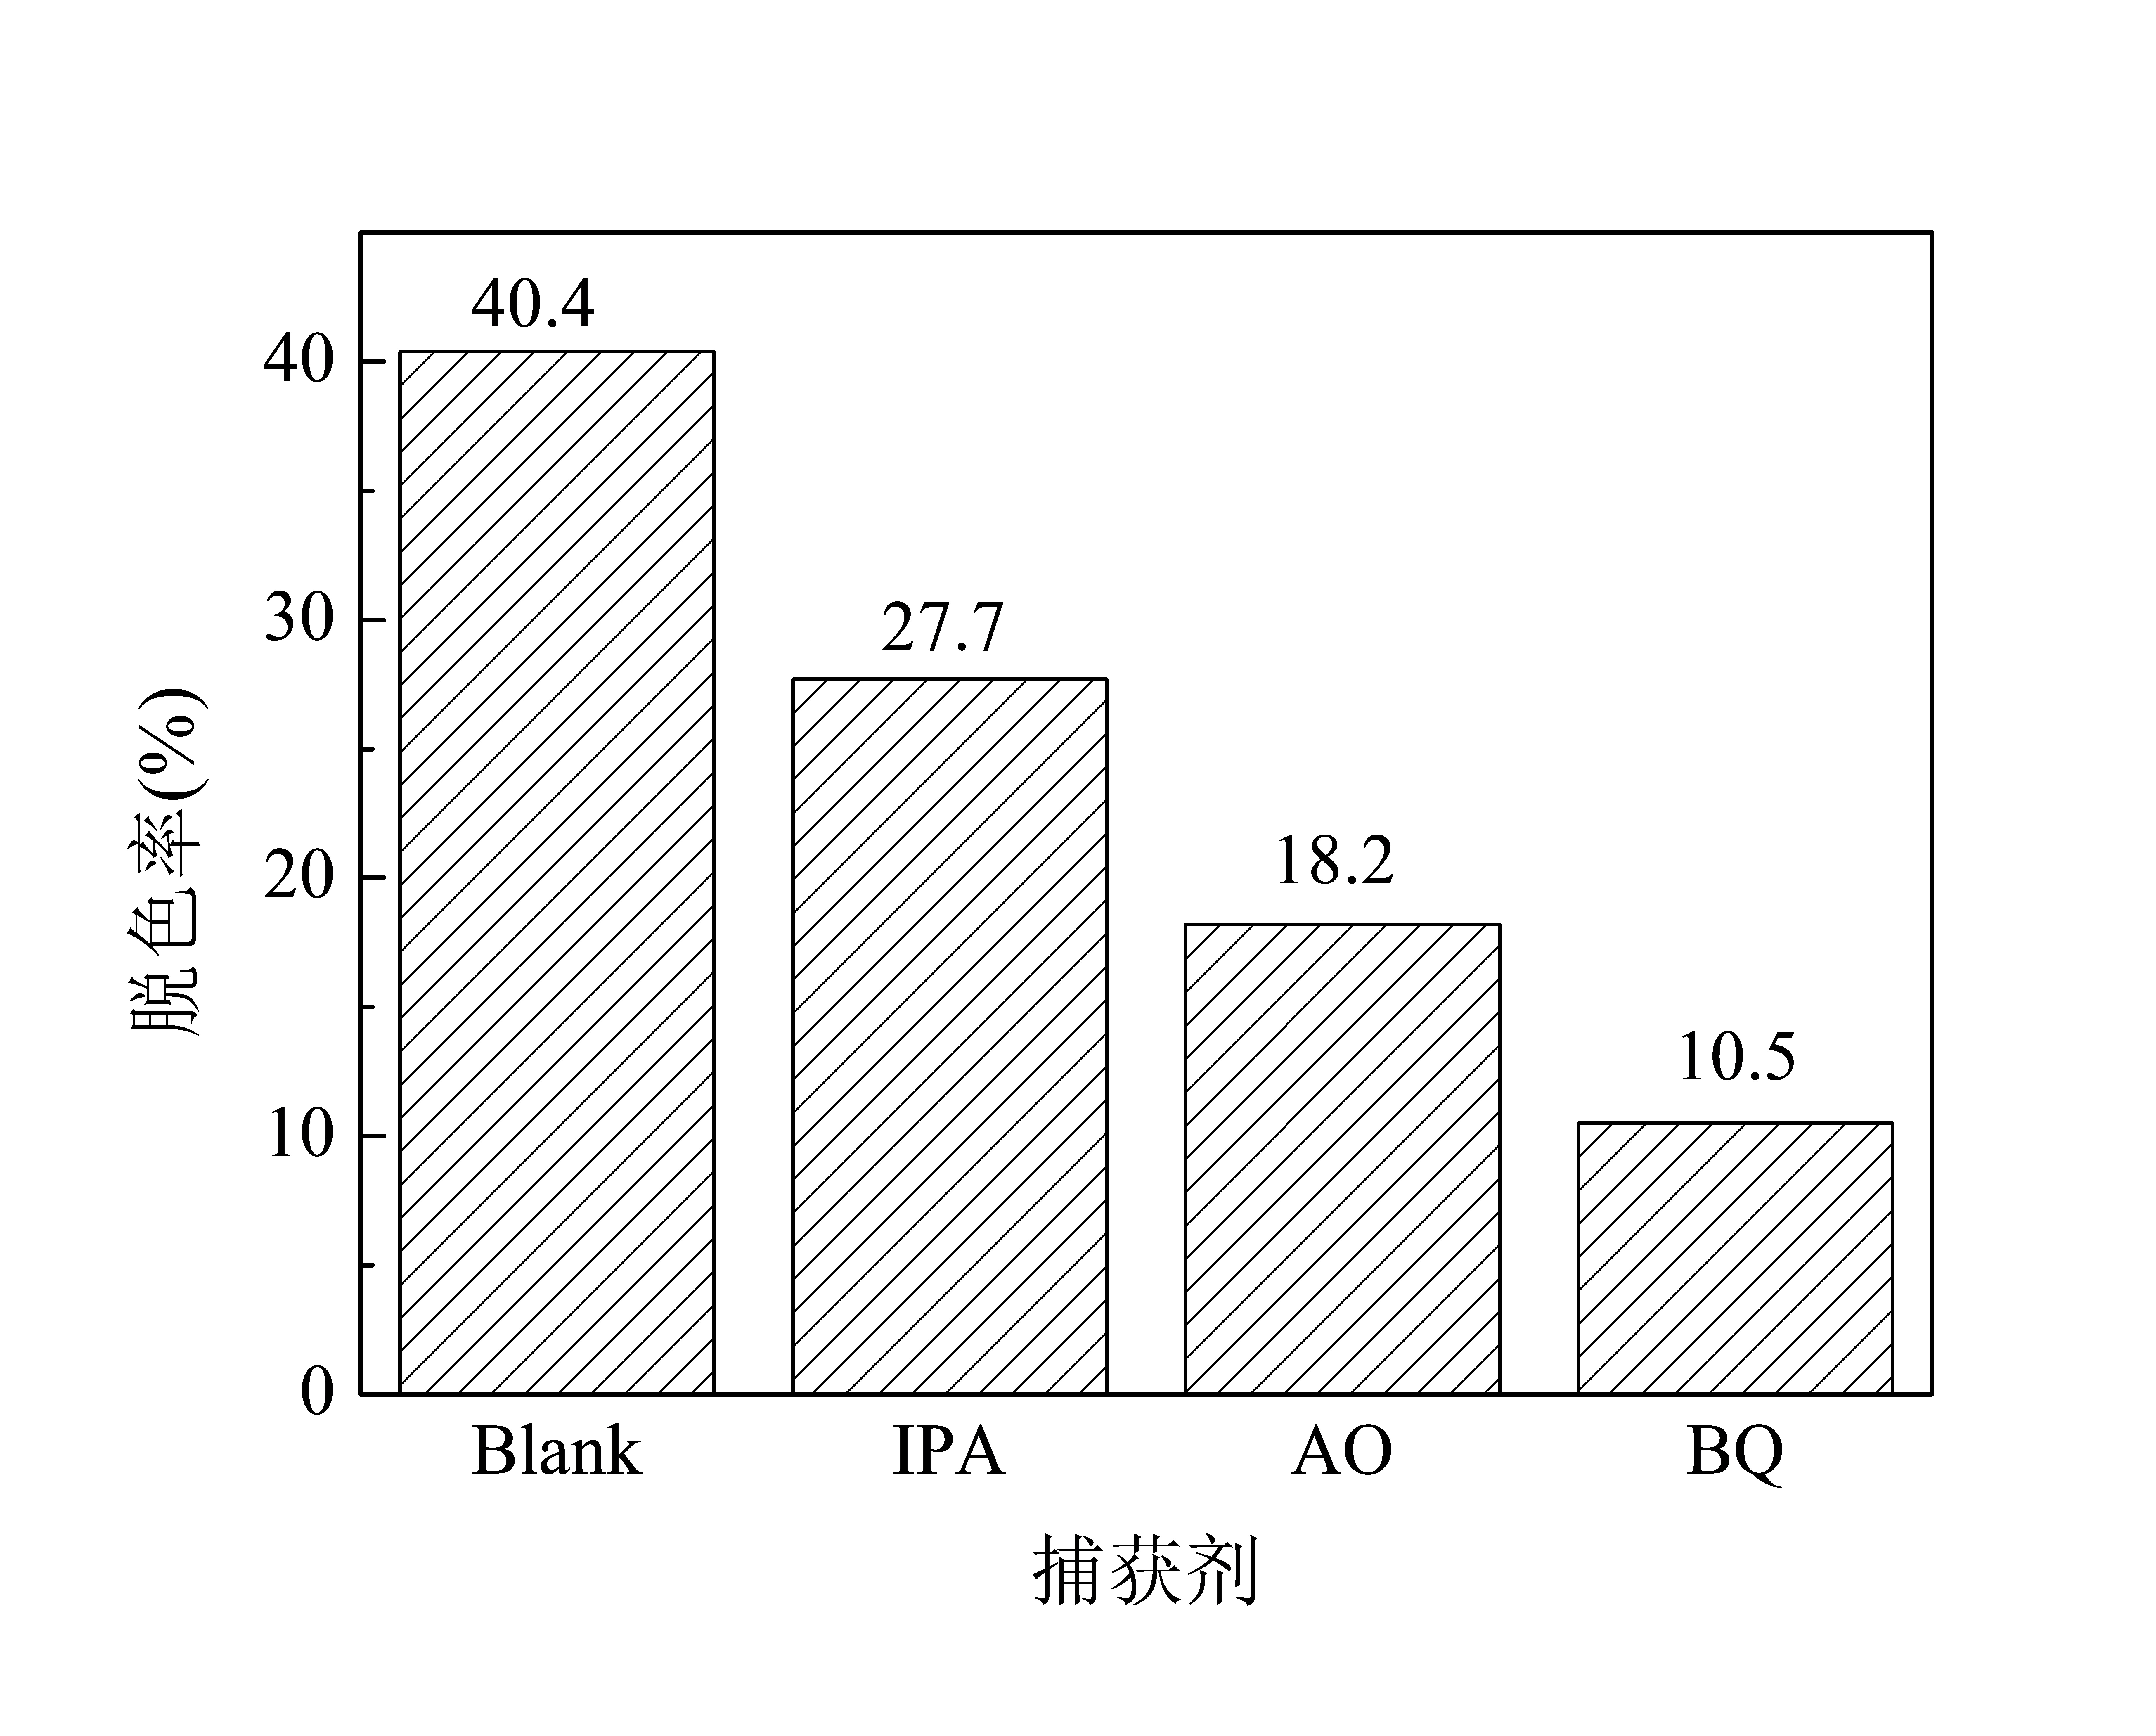
\includegraphics[width=\linewidth]{figures/三氧化二铟捕获剂.jpg} 
\end{block}
\column{0.5\textwidth}
\begin{block}{}
加入苯琨后甲基橙脱色率由 40.4\%急剧下降至 10.5\%,这表明•O$ \mathbf{^{2-}} $是主要的活性自由基,加入异丙醇和草酸铵后甲基橙脱色率由 40.4\%分别下降至 18.2 和 27.7\%,这说明•OH 和 h+起次要作用。
\end{block}
\end{columns}
\end{frame}

\begin{frame}
\frametitle{\chemfig{\mathbf{In_2O_3/ Bi_2O_3}}光催化剂的SPS图谱}
\begin{block}{}
\centering
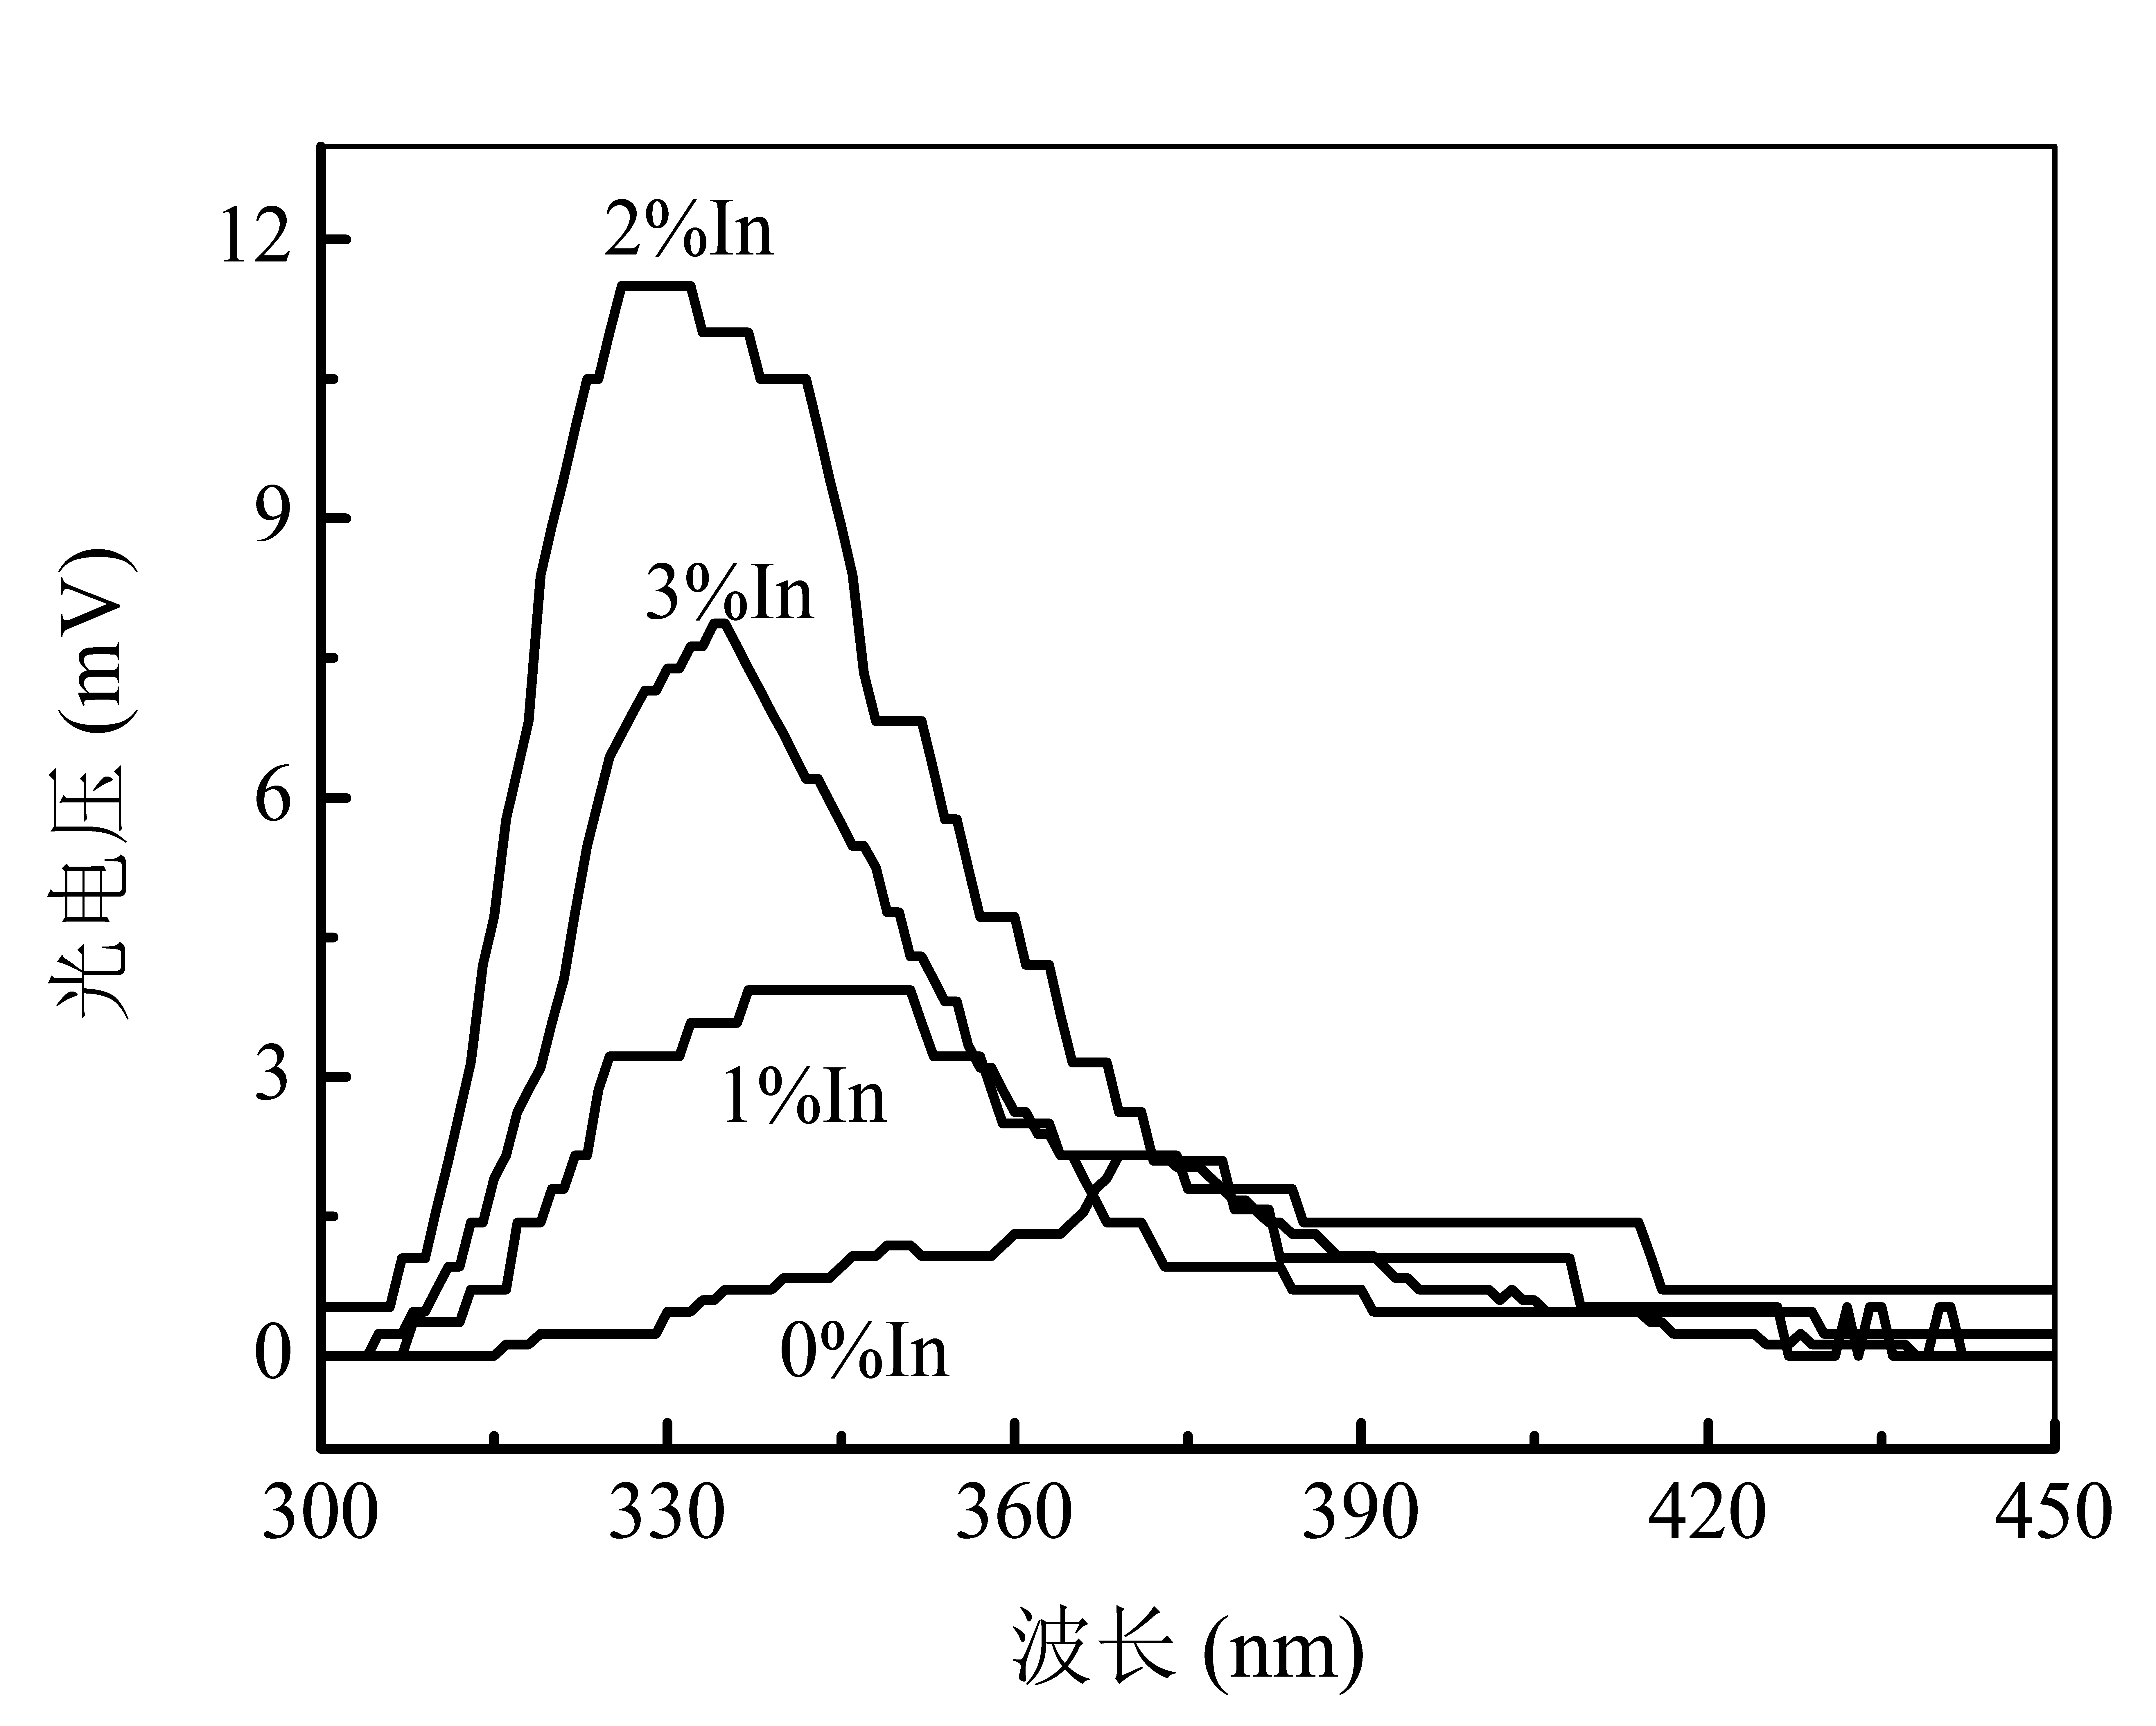
\includegraphics[width=0.8\textwidth]{figures/三氧化二铟SPS.jpg} 
\end{block}
\end{frame}

\begin{frame}
\frametitle{\chemfig{\mathbf{In_2O_3/ Bi_2O_3}}光催化剂的光催化活性}
\begin{block}{}
\centering
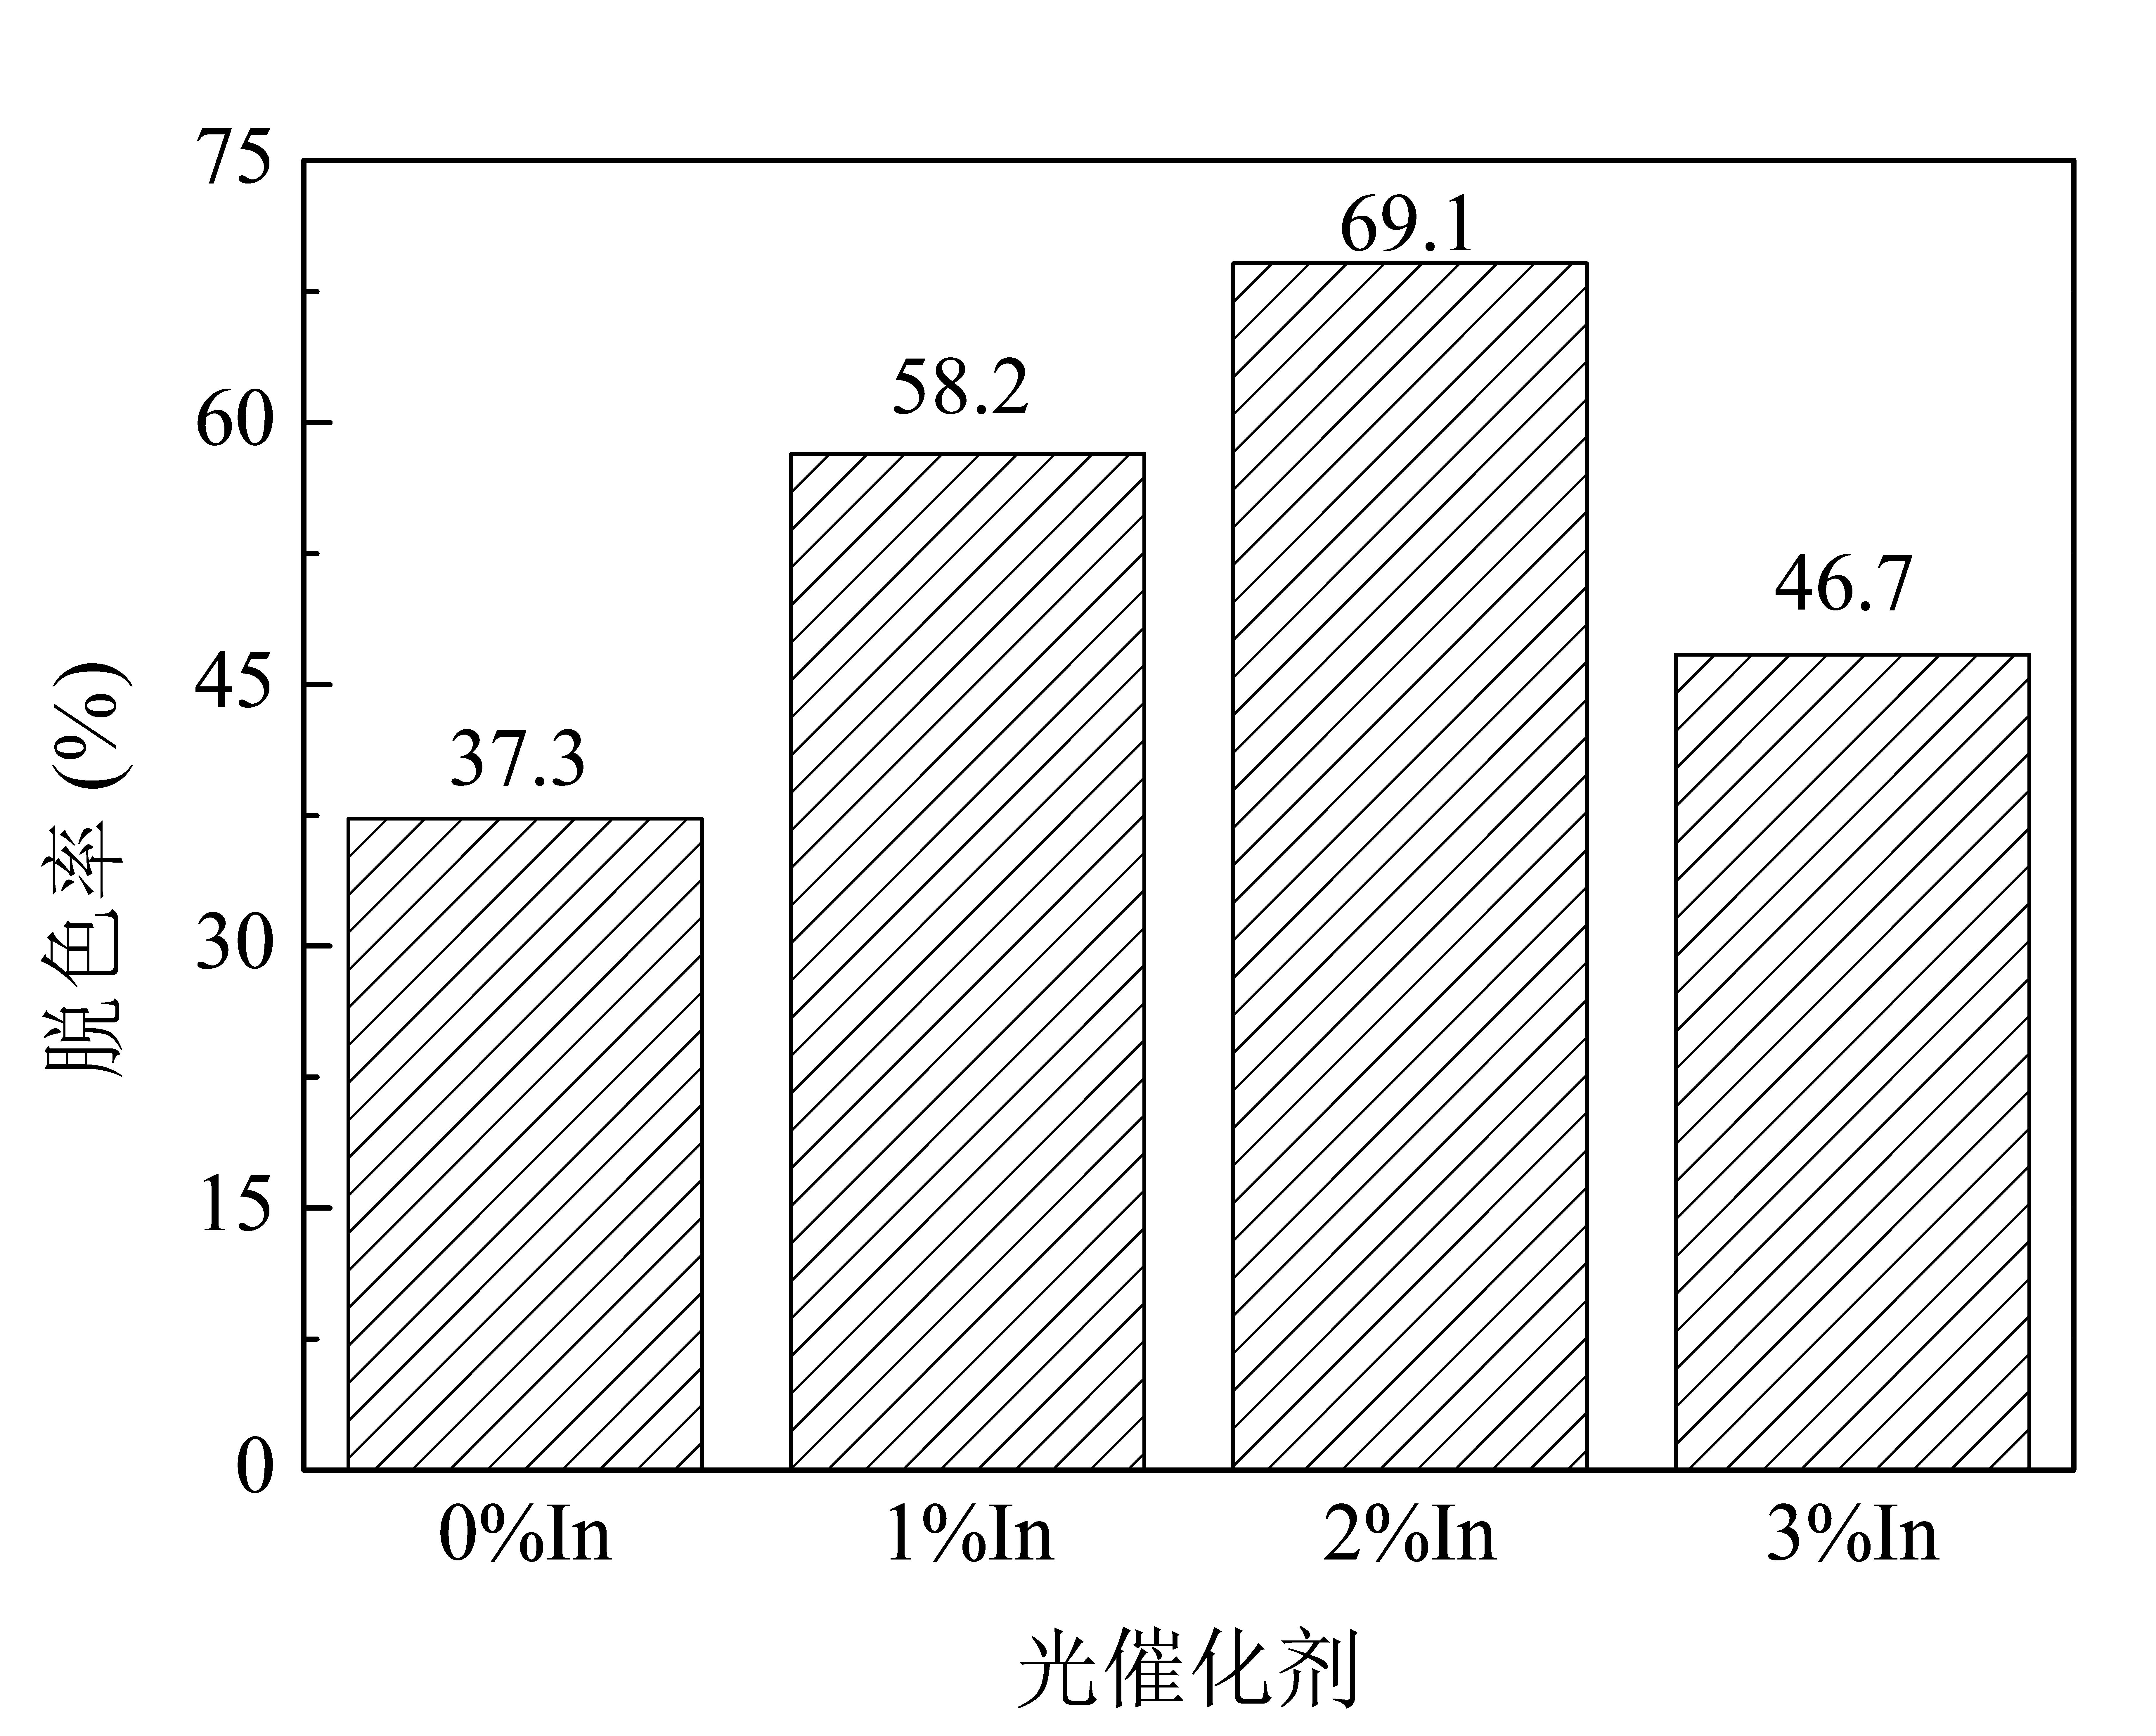
\includegraphics[width=0.8\textwidth]{figures/三氧化二铟脱色率.jpg} 
\end{block}
\end{frame}

%%<1>  first show <2> second show [<+->]依次显示 <1-2>1,2都显示 <1->从1一直显示
\begin{frame}
\frametitle{\chemfig{\mathbf{In_2O_3/ Bi_2O_3}}光催化剂研究总结}
\begin{block}{}
\begin{itemize}
\item 在\chemfig{\mathbf{Bi_2O_3}}表面负载\chemfig{\mathbf{In_2O_3}}后表征结果显示形成了\chemfig{\mathbf{In_2O_3/ Bi_2O_3}}异质结,\chemfig{\mathbf{In_2O_3}}和\chemfig{\mathbf{Bi_2O_3}}存在强的耦合作用,从而光生载流子分离效应增强,在日光照射下所制备异质结对甲基橙光催化活性得到显著提高,其In/Bi原子比为2\%时样品具有最好的太阳光催化活性。%pause
\end{itemize}
\end{block}
\end{frame}

\subsection{三氧化二铁}
\begin{frame}
\frametitle{\chemfig{\mathbf{Fe_2O_3/Bi_2O_3}}光催化剂的比表面积}
\centering
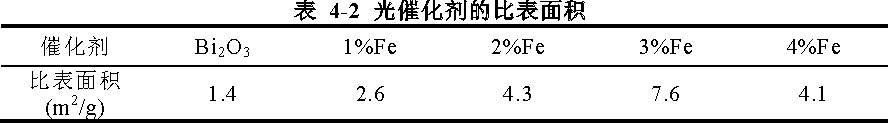
\includegraphics[width=\textwidth]{figures/三氧化二铁比表面积.pdf} 
\begin{block}{}
随\chemfig{\mathbf{Fe_2O_3}}负载量逐渐增加,光催化剂比表面逐渐增加,当 Fe/Bi 摩尔比为 3\%时,催化剂的比表面最大,进一步增加\chemfig{\mathbf{Fe_2O_3}}负载量比表面下降。\chemfig{\mathbf{Fe_2O_3}}的负载量较低时比表面较小;而\chemfig{\mathbf{Fe_2O_3}}的负载量过高时,大量的\chemfig{\mathbf{Fe_2O_3}}在原有表面重复堆积,堵塞载体孔道,使比表面减少。
\end{block}
\end{frame}

\begin{frame}
\frametitle{\chemfig{\mathbf{Fe_2O_3/Bi_2O_3}}光催化剂的XRD图谱}
\begin{block}{}
\centering
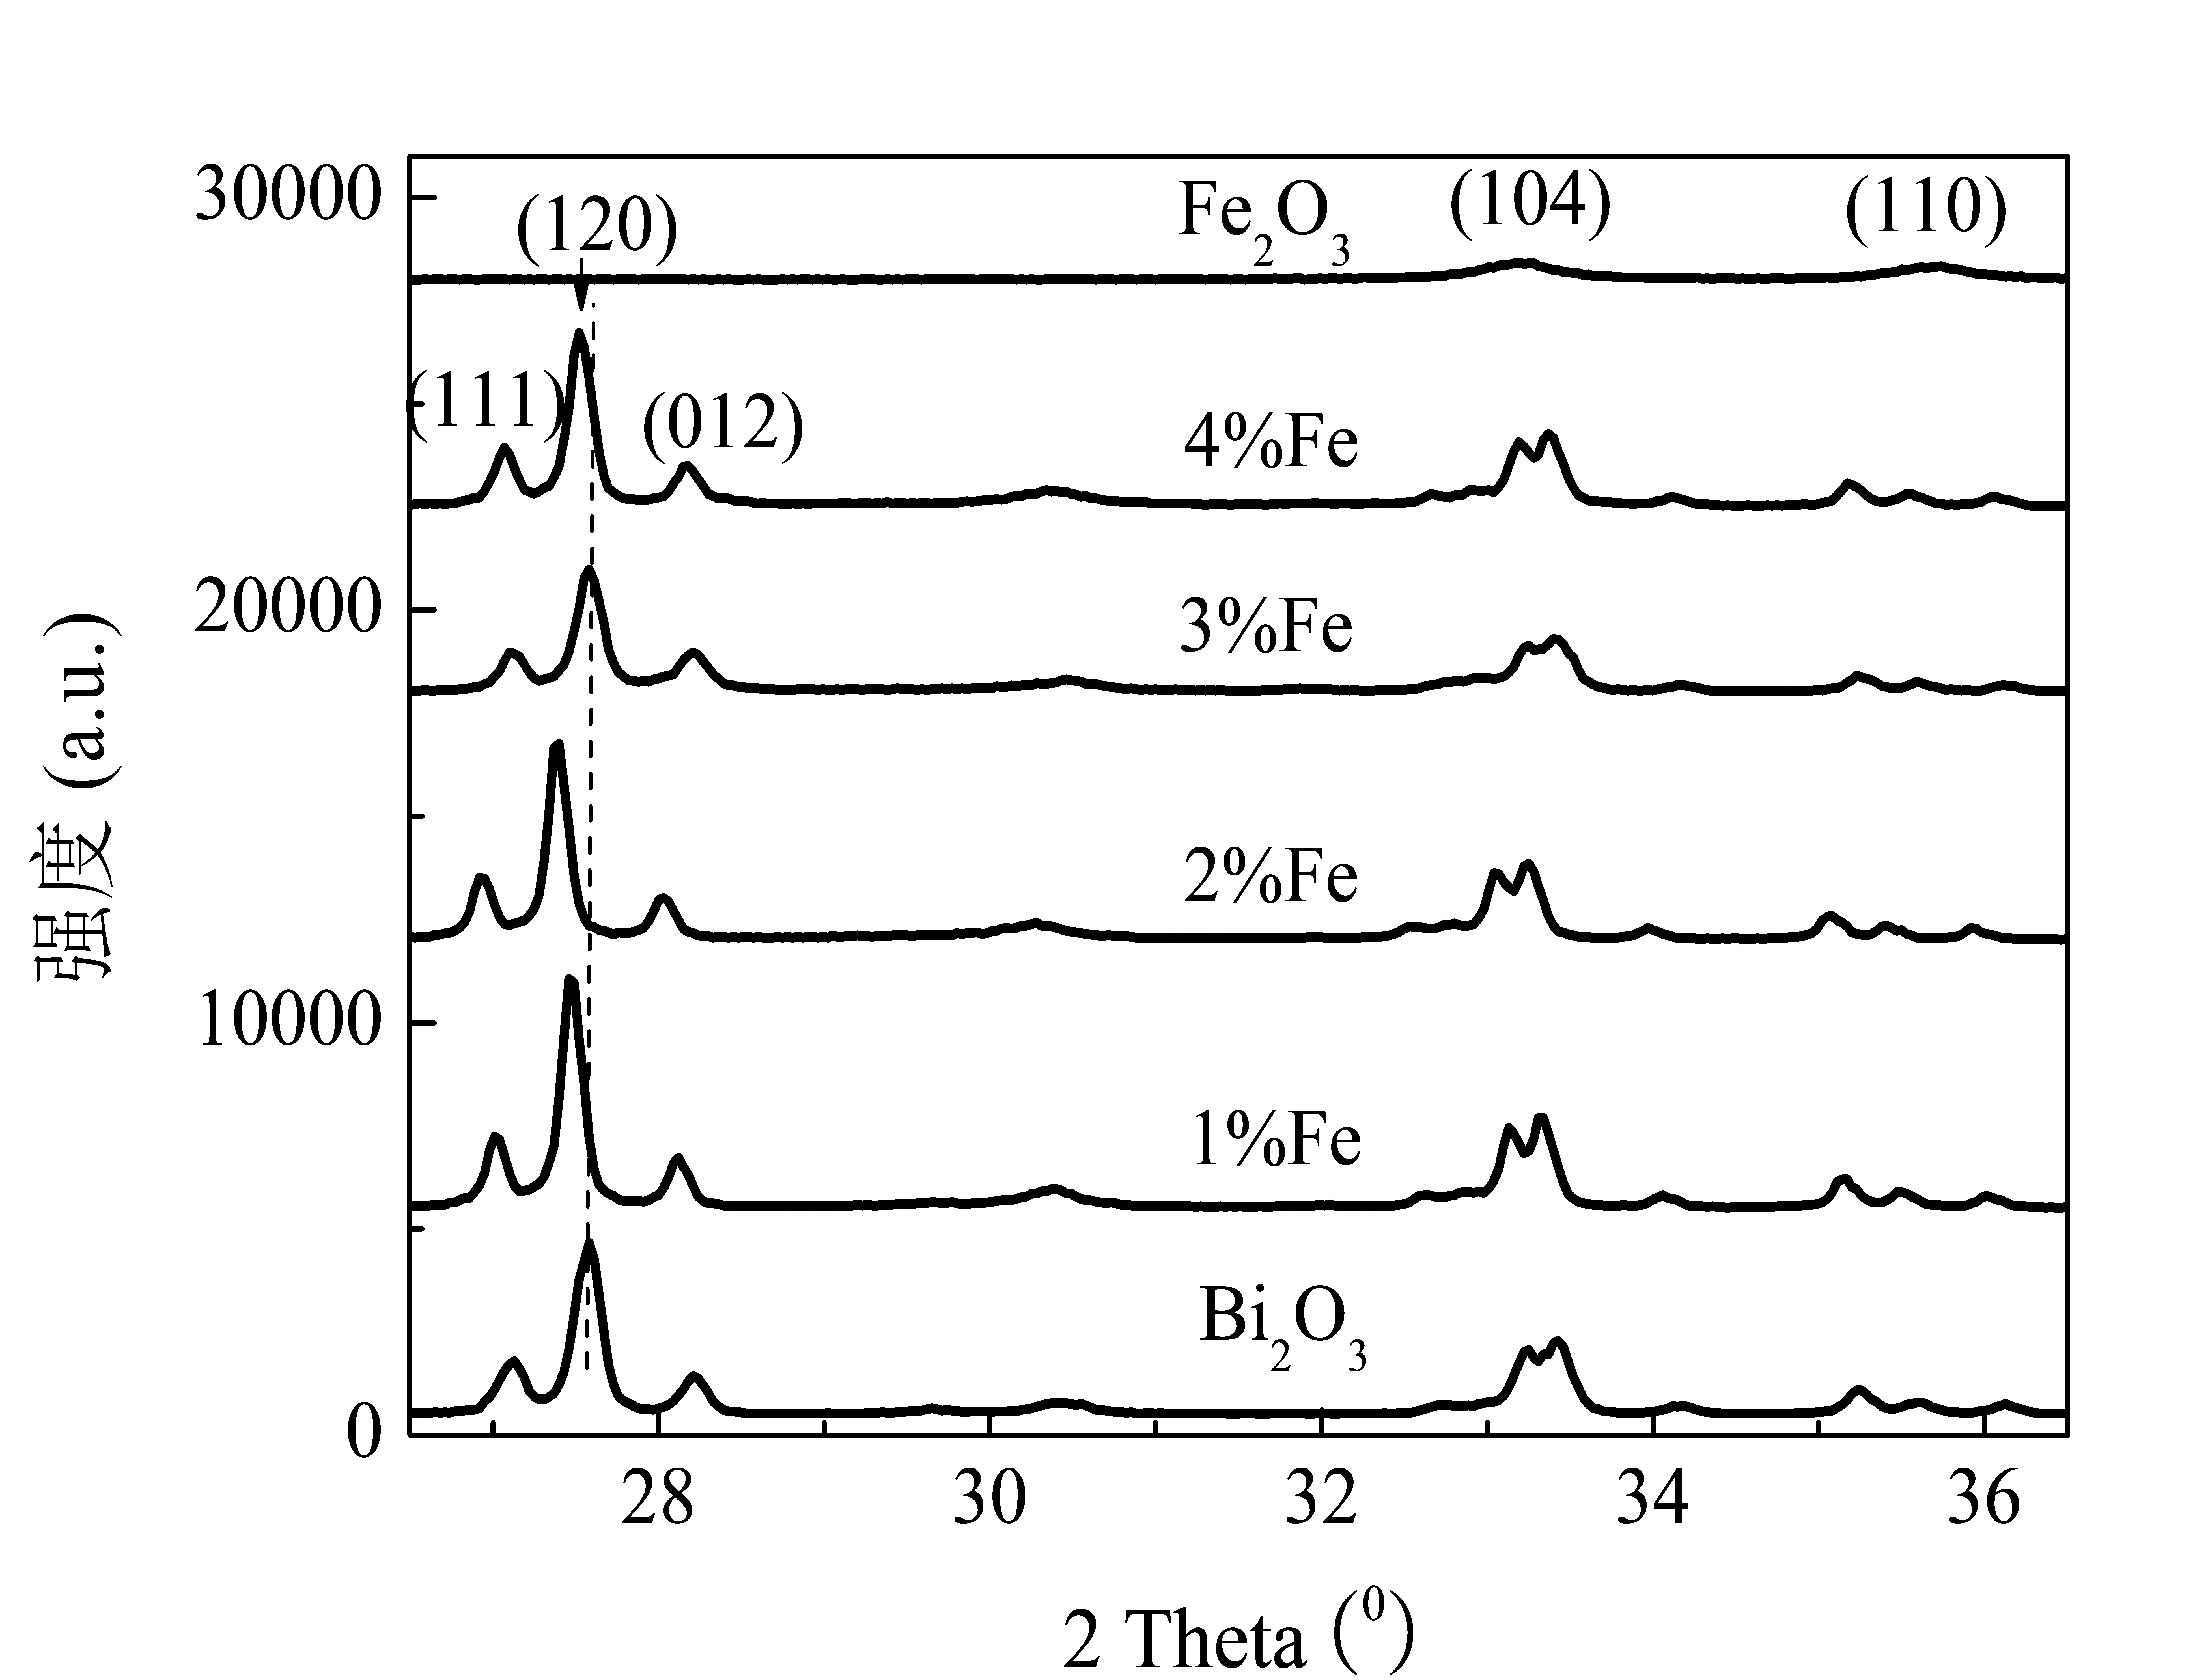
\includegraphics[width=0.85\textwidth]{figures/三氧化二铁XRD} 
\end{block}
\end{frame}

\begin{frame}
\frametitle{\chemfig{\mathbf{Fe_2O_3/Bi_2O_3}}光催化剂的UV-Vis图谱}
\begin{block}{}
\centering
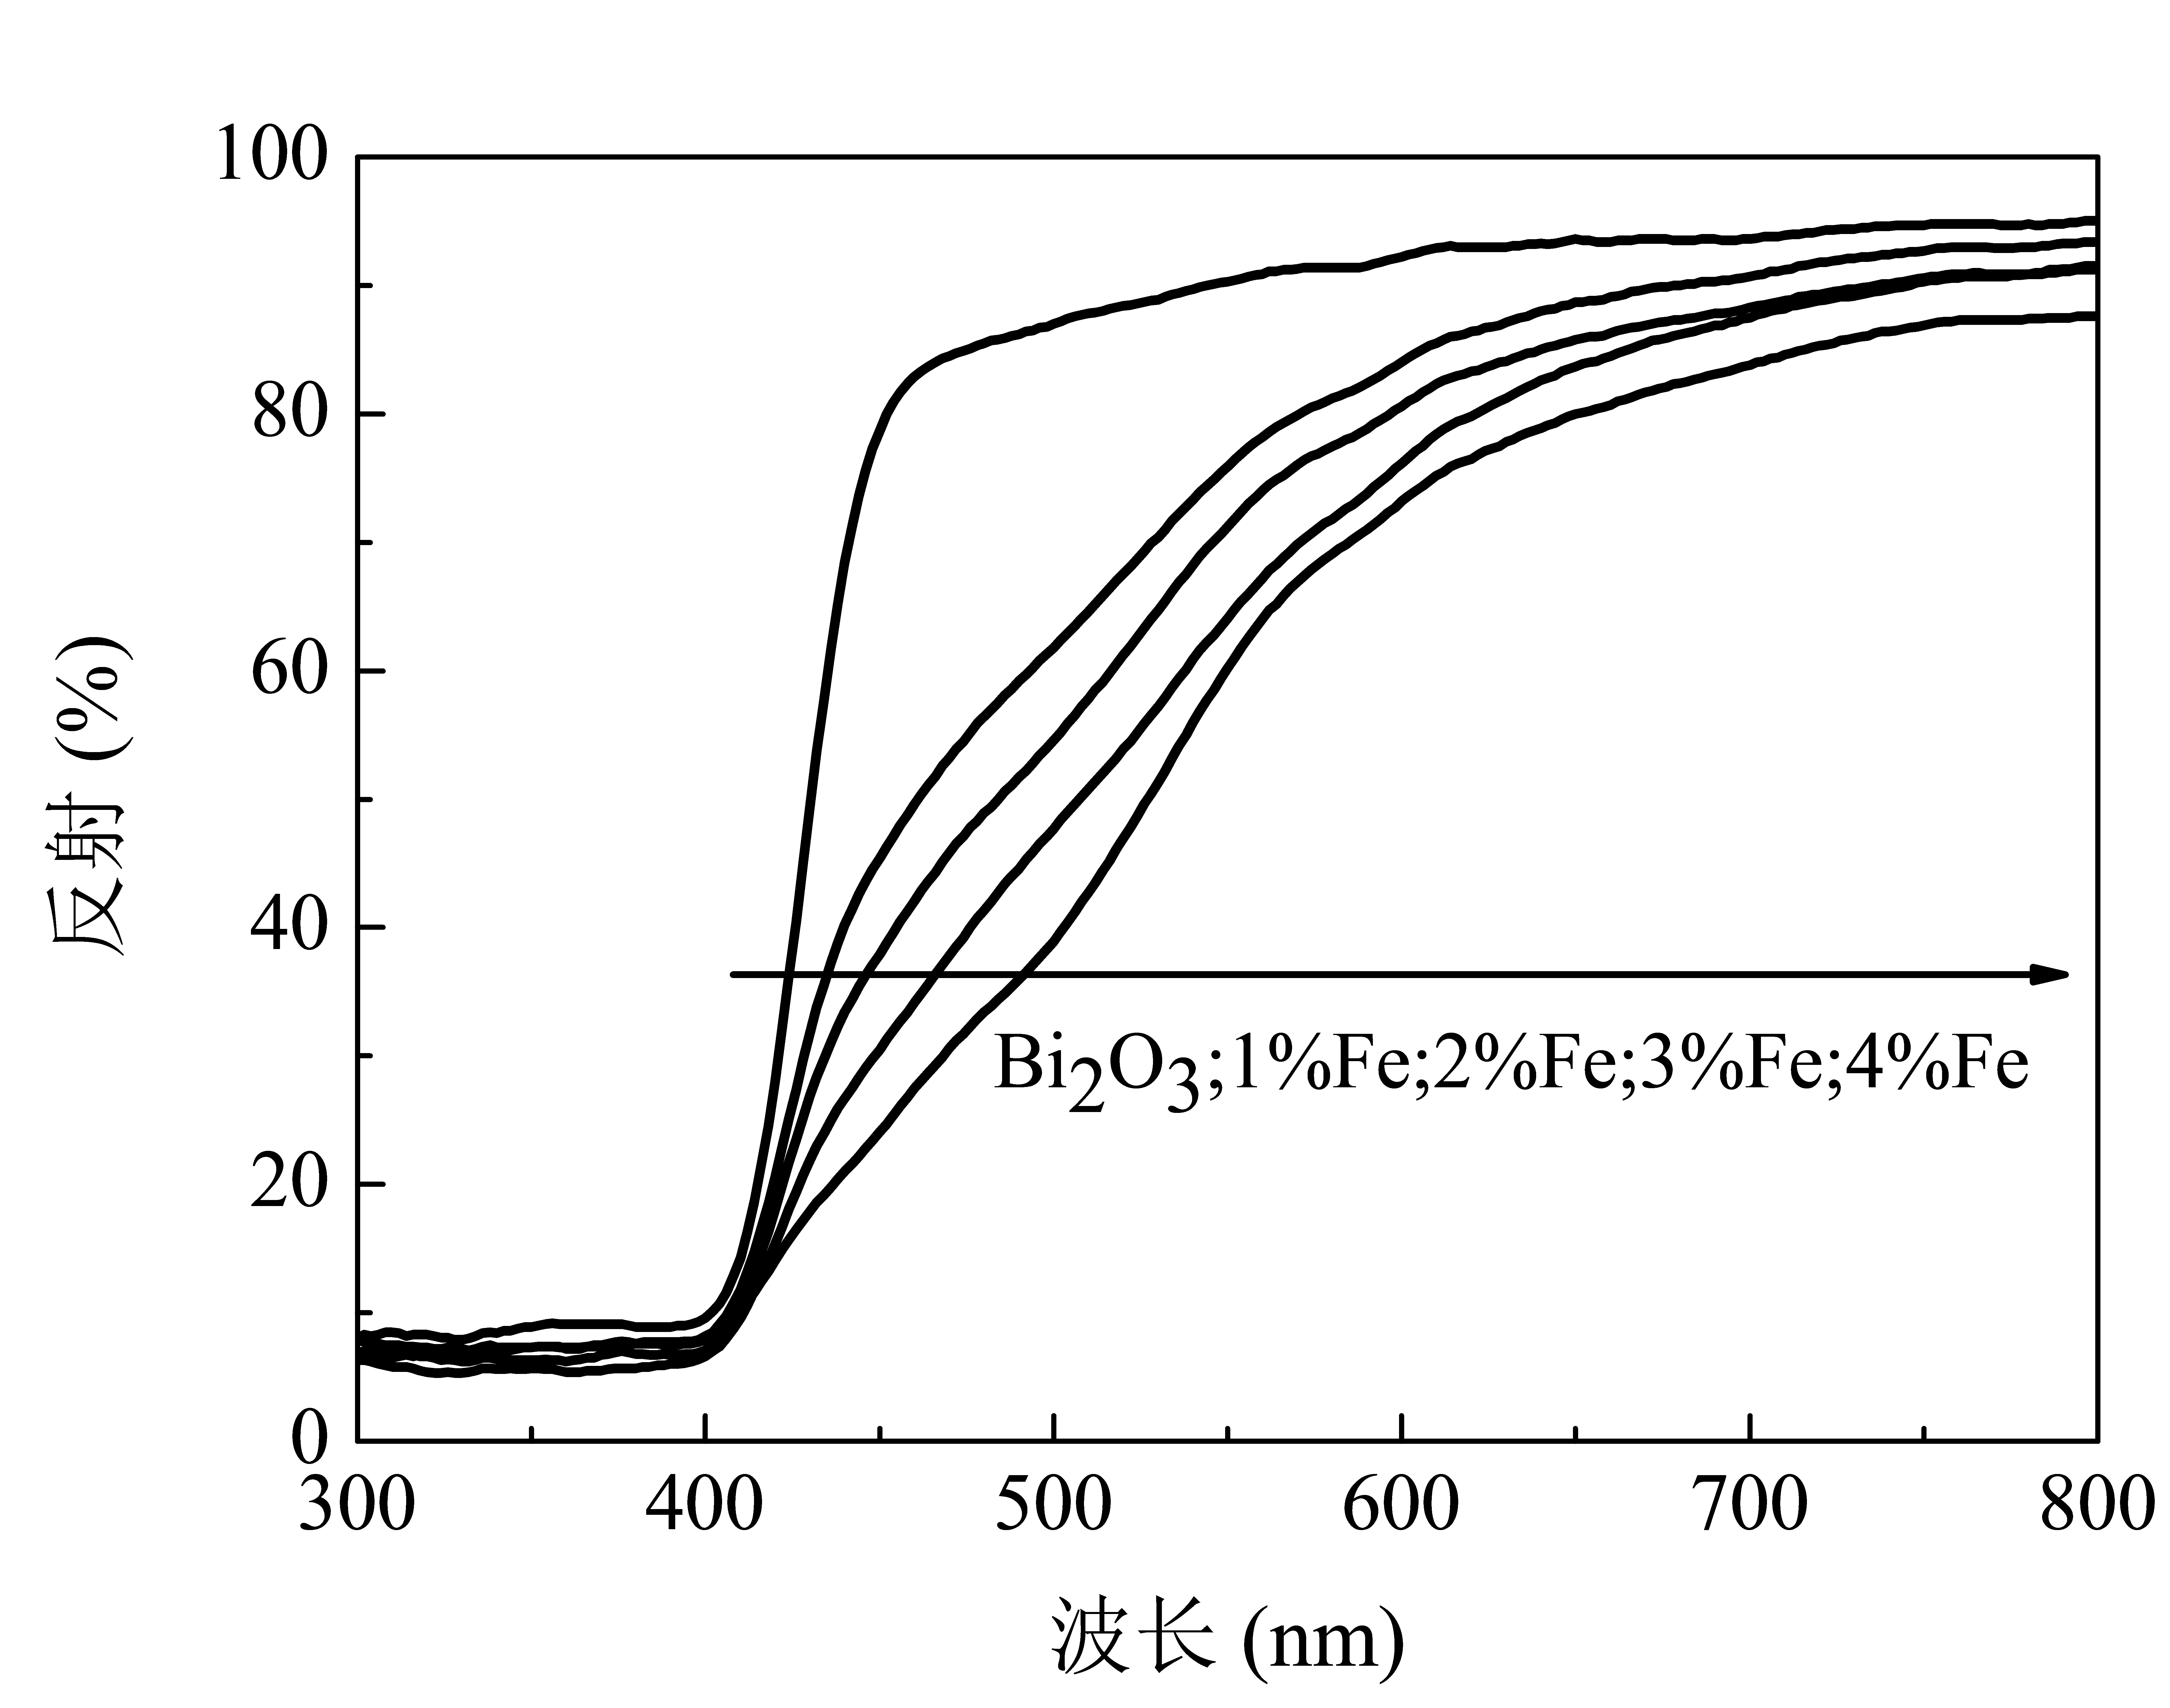
\includegraphics[width=0.8\textwidth]{figures/三氧化二铁UV.jpg} 
\end{block}
\end{frame}

\begin{frame}
\frametitle{\chemfig{\mathbf{Fe_2O_3/Bi_2O_3}}光催化剂的XPS图谱}
\begin{block}{}
\centering
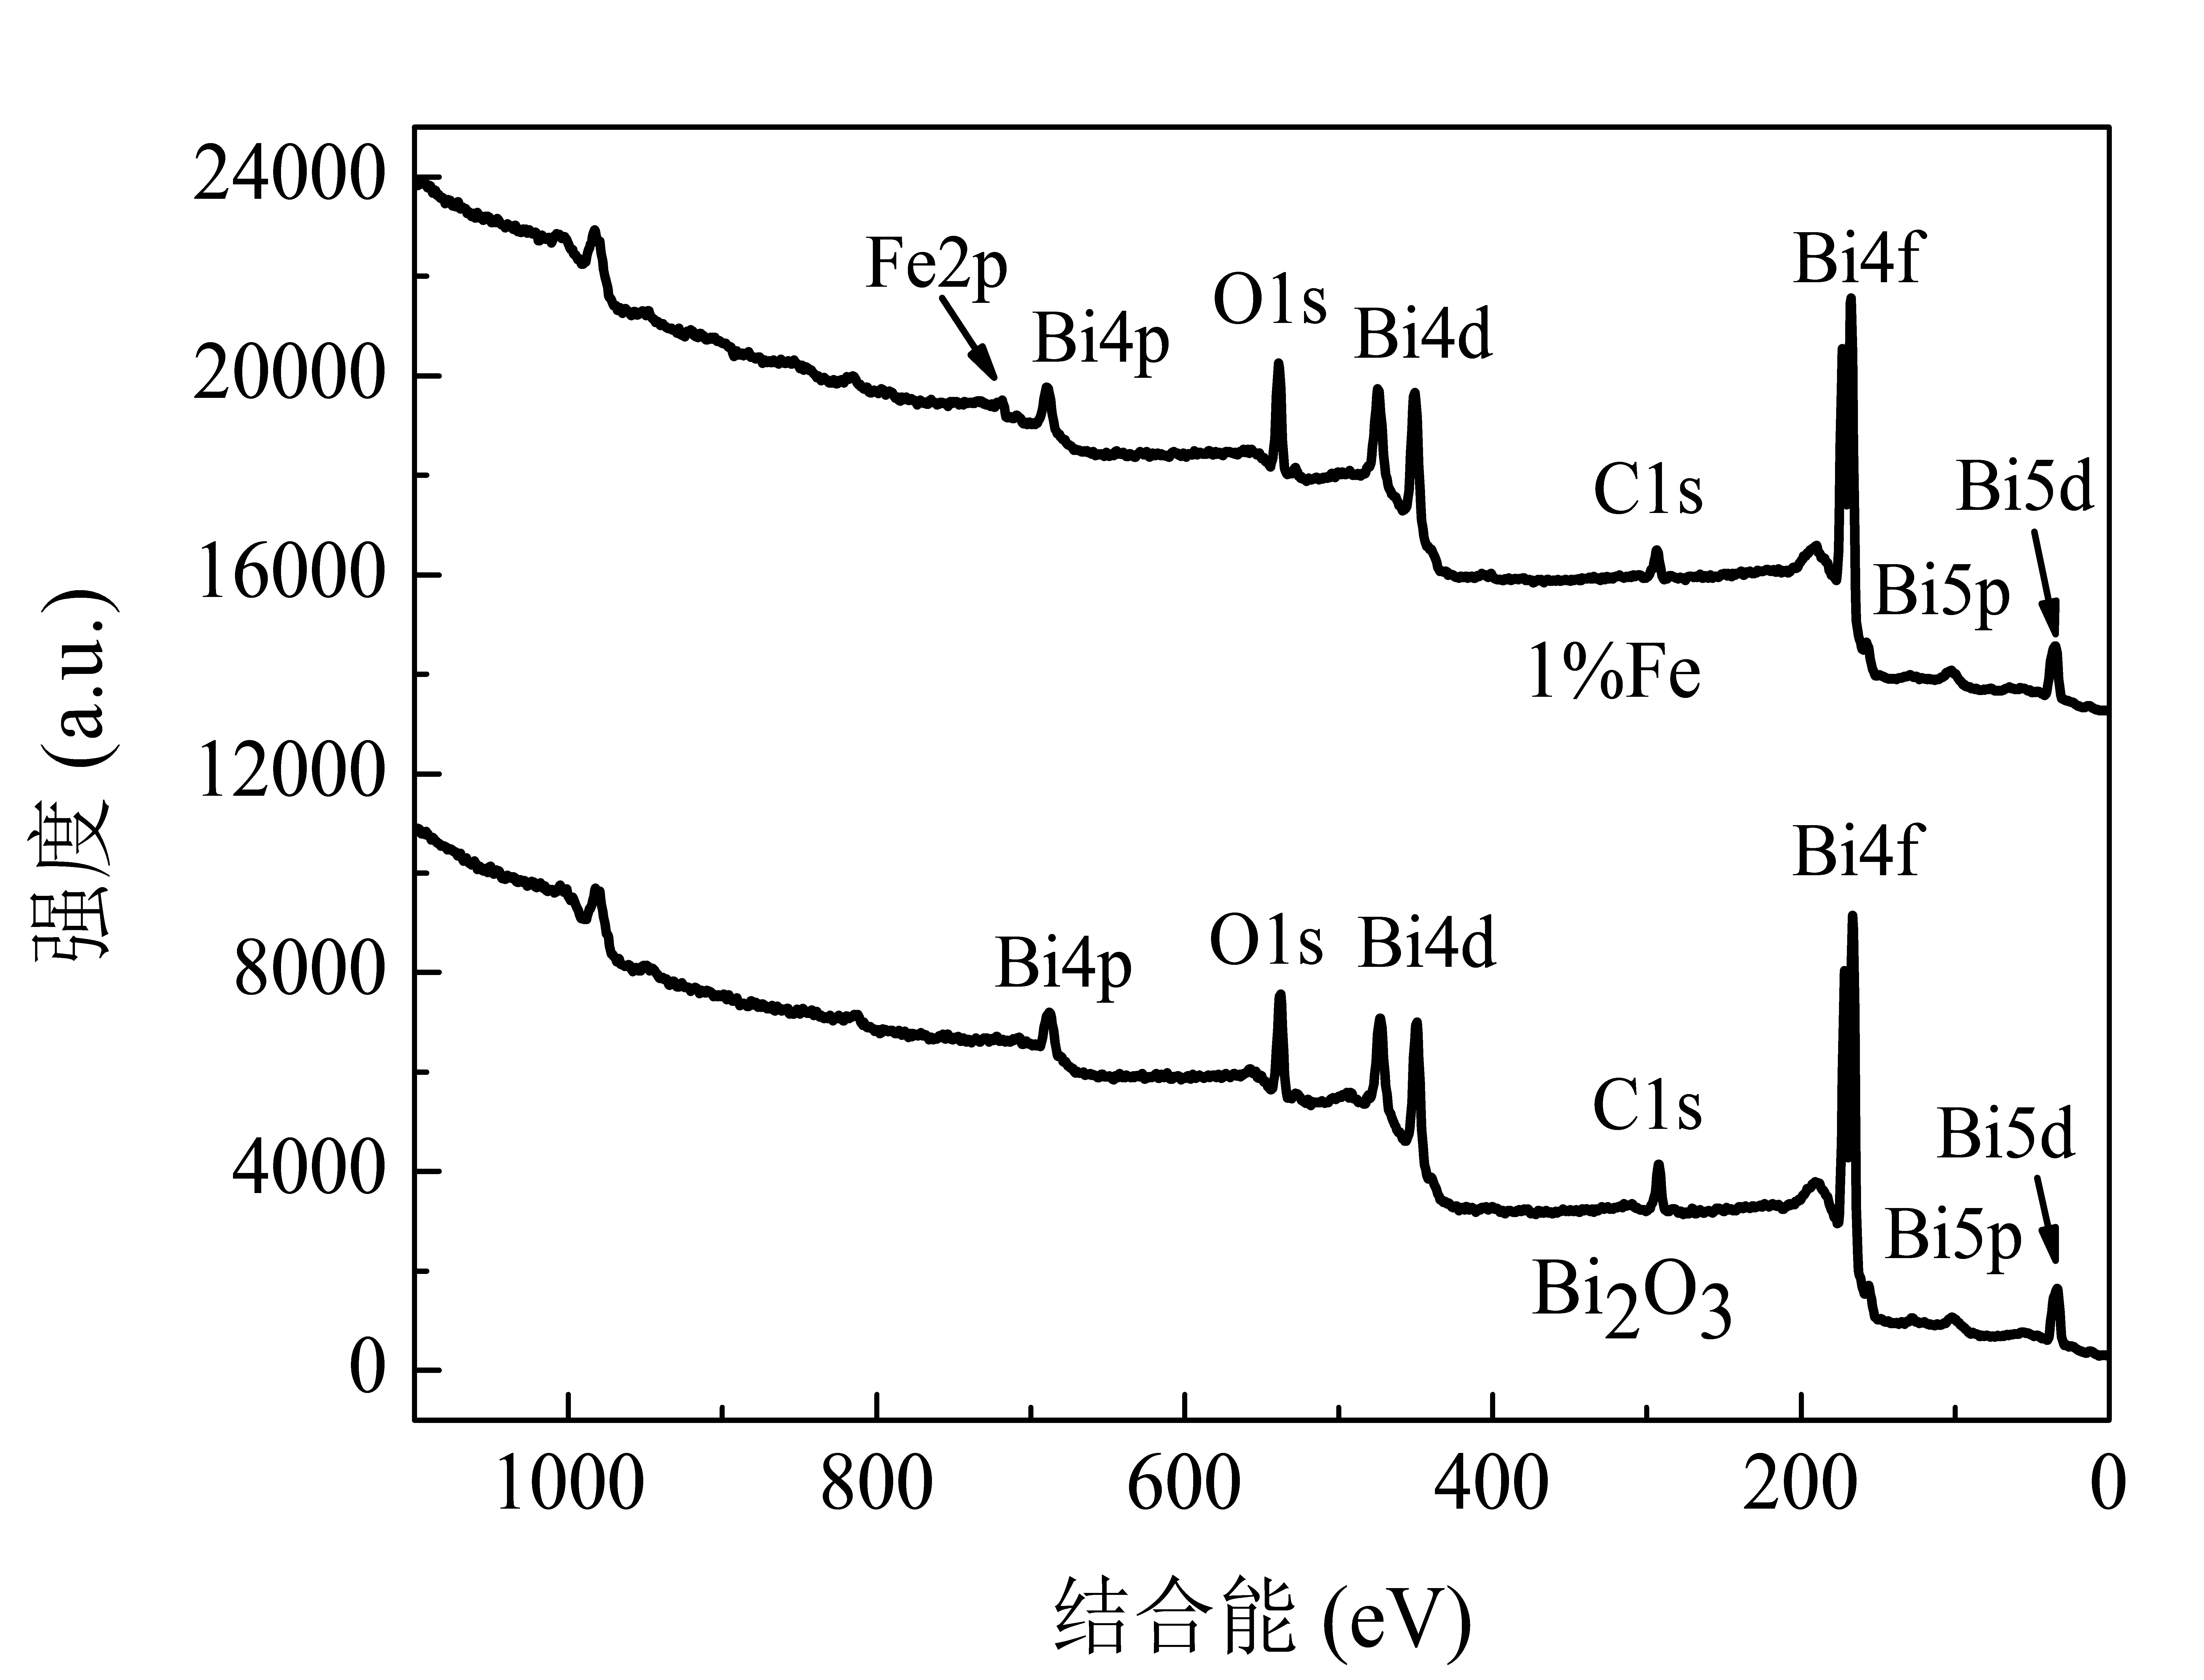
\includegraphics[width=0.8\textwidth]{figures/三氧化二铁XPS.jpg} 
\end{block}
\end{frame}

\begin{frame}
\frametitle{\chemfig{\mathbf{Fe_2O_3/Bi_2O_3}}光催化剂的XPS图谱分析一}
\begin{columns}
\column{0.6\textwidth}
\begin{block}{}
\centering
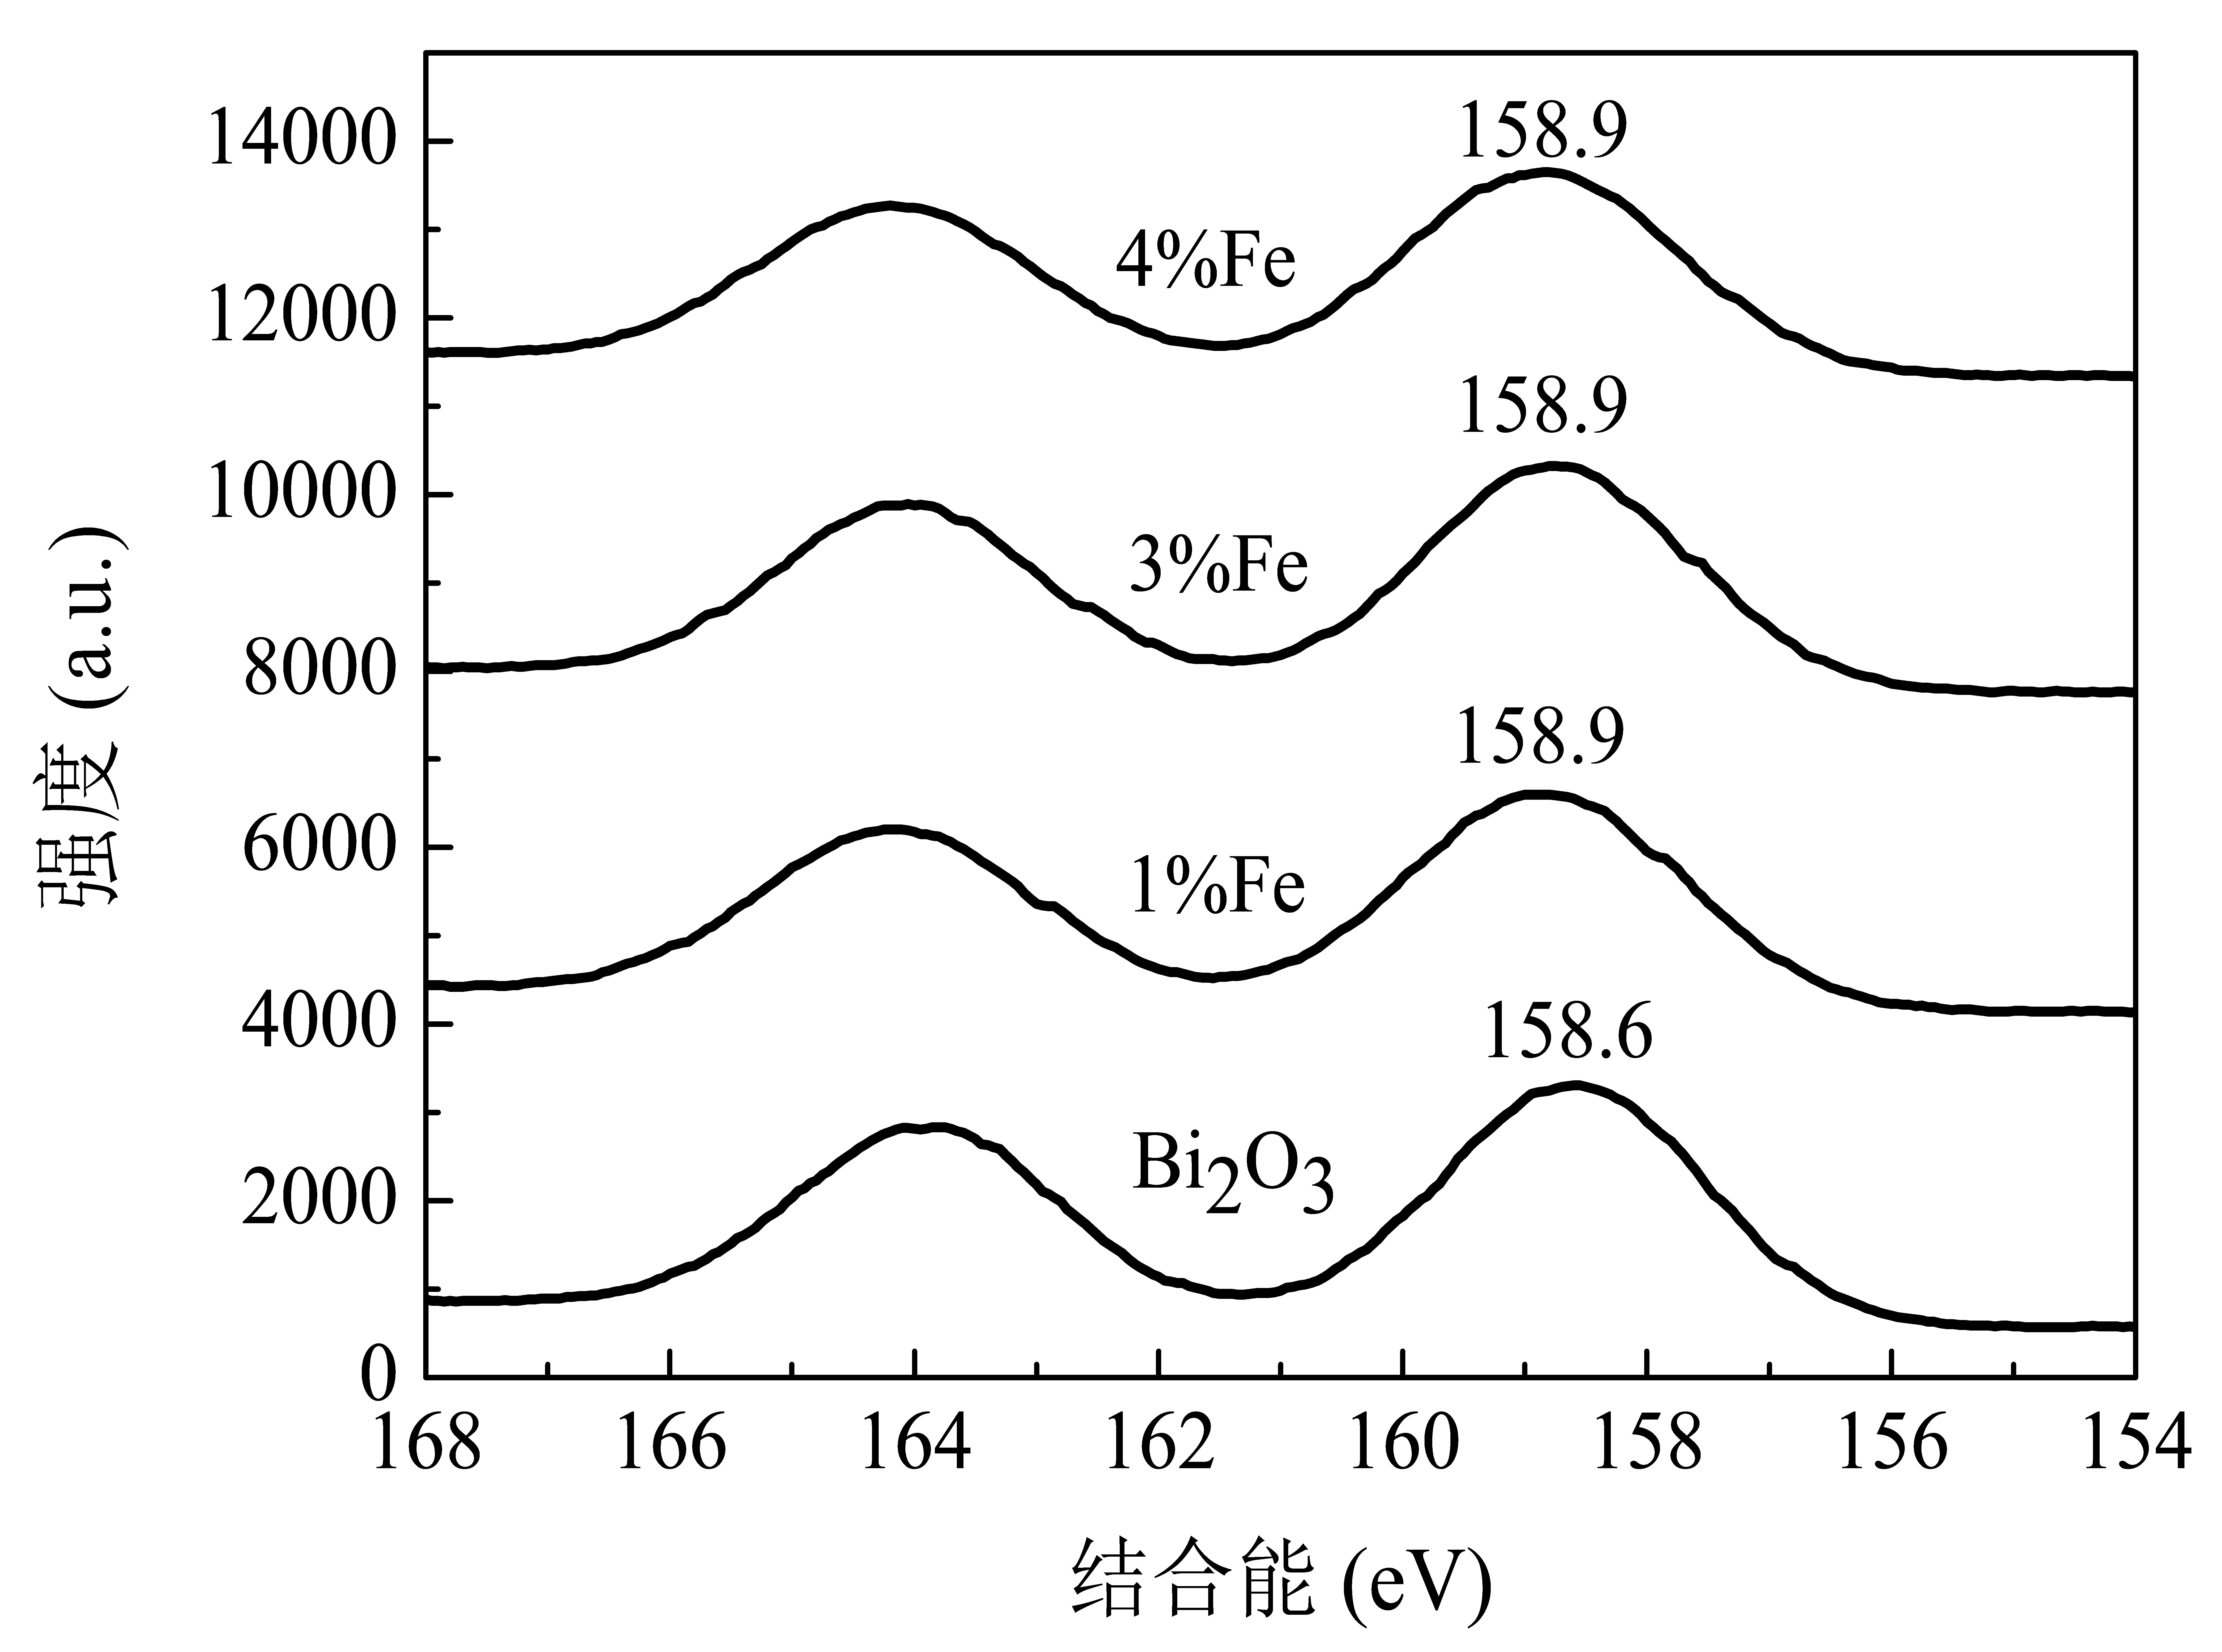
\includegraphics[width=\linewidth]{figures/三氧化二铁BI4F.jpg} 
\end{block}
\column{0.4\textwidth}
\begin{block}{Bi4f轨道分析}
对于纯\chemfig{\mathbf{Bi_2O_3}},Bi4f7/2 位于 158.6 eV,表明 Bi 是 3+。然而,对负载型光催化剂,Bi4f7/2 向高能端偏移,这表明\chemfig{\mathbf{Bi_2O_3}}和\chemfig{\mathbf{Fe_2O_3}}之间发生了相互作用。
\end{block}
\end{columns}
\end{frame}


\begin{frame}
\frametitle{\chemfig{\mathbf{Fe_2O_3/Bi_2O_3}}光催化剂的XPS图谱分析二}
\begin{columns}
\column{0.6\textwidth}
\begin{block}{}
\centering
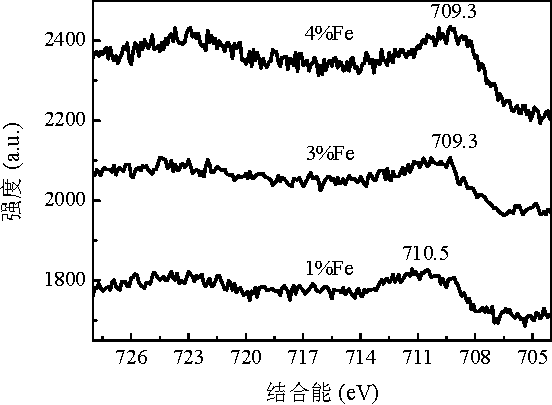
\includegraphics[width=\linewidth]{figures/三氧化二铁2P} 
\end{block}
\column{0.4\textwidth}
\begin{block}{In3d轨道分析}
根据文献报道 710.5 eV 对应于\chemfig{\mathbf{Fe^{3+}}}的 Fe 2p3/2  ,然而随着\chemfig{\mathbf{Fe_2O_3}}负载量的增加,Fe2p3/2 向低能端偏移,这对应于 Bi4f7/2 向高能端偏移,该结果进一步表明\chemfig{\mathbf{Bi_2O_3}}和\chemfig{\mathbf{Fe_2O_3}}之间发生了相互作用。
\end{block}
\end{columns}
\end{frame}

\begin{frame}
\frametitle{捕获剂对催化剂脱色率的影响}
\begin{columns}
\column{0.5\textwidth}
\begin{block}{}
\centering
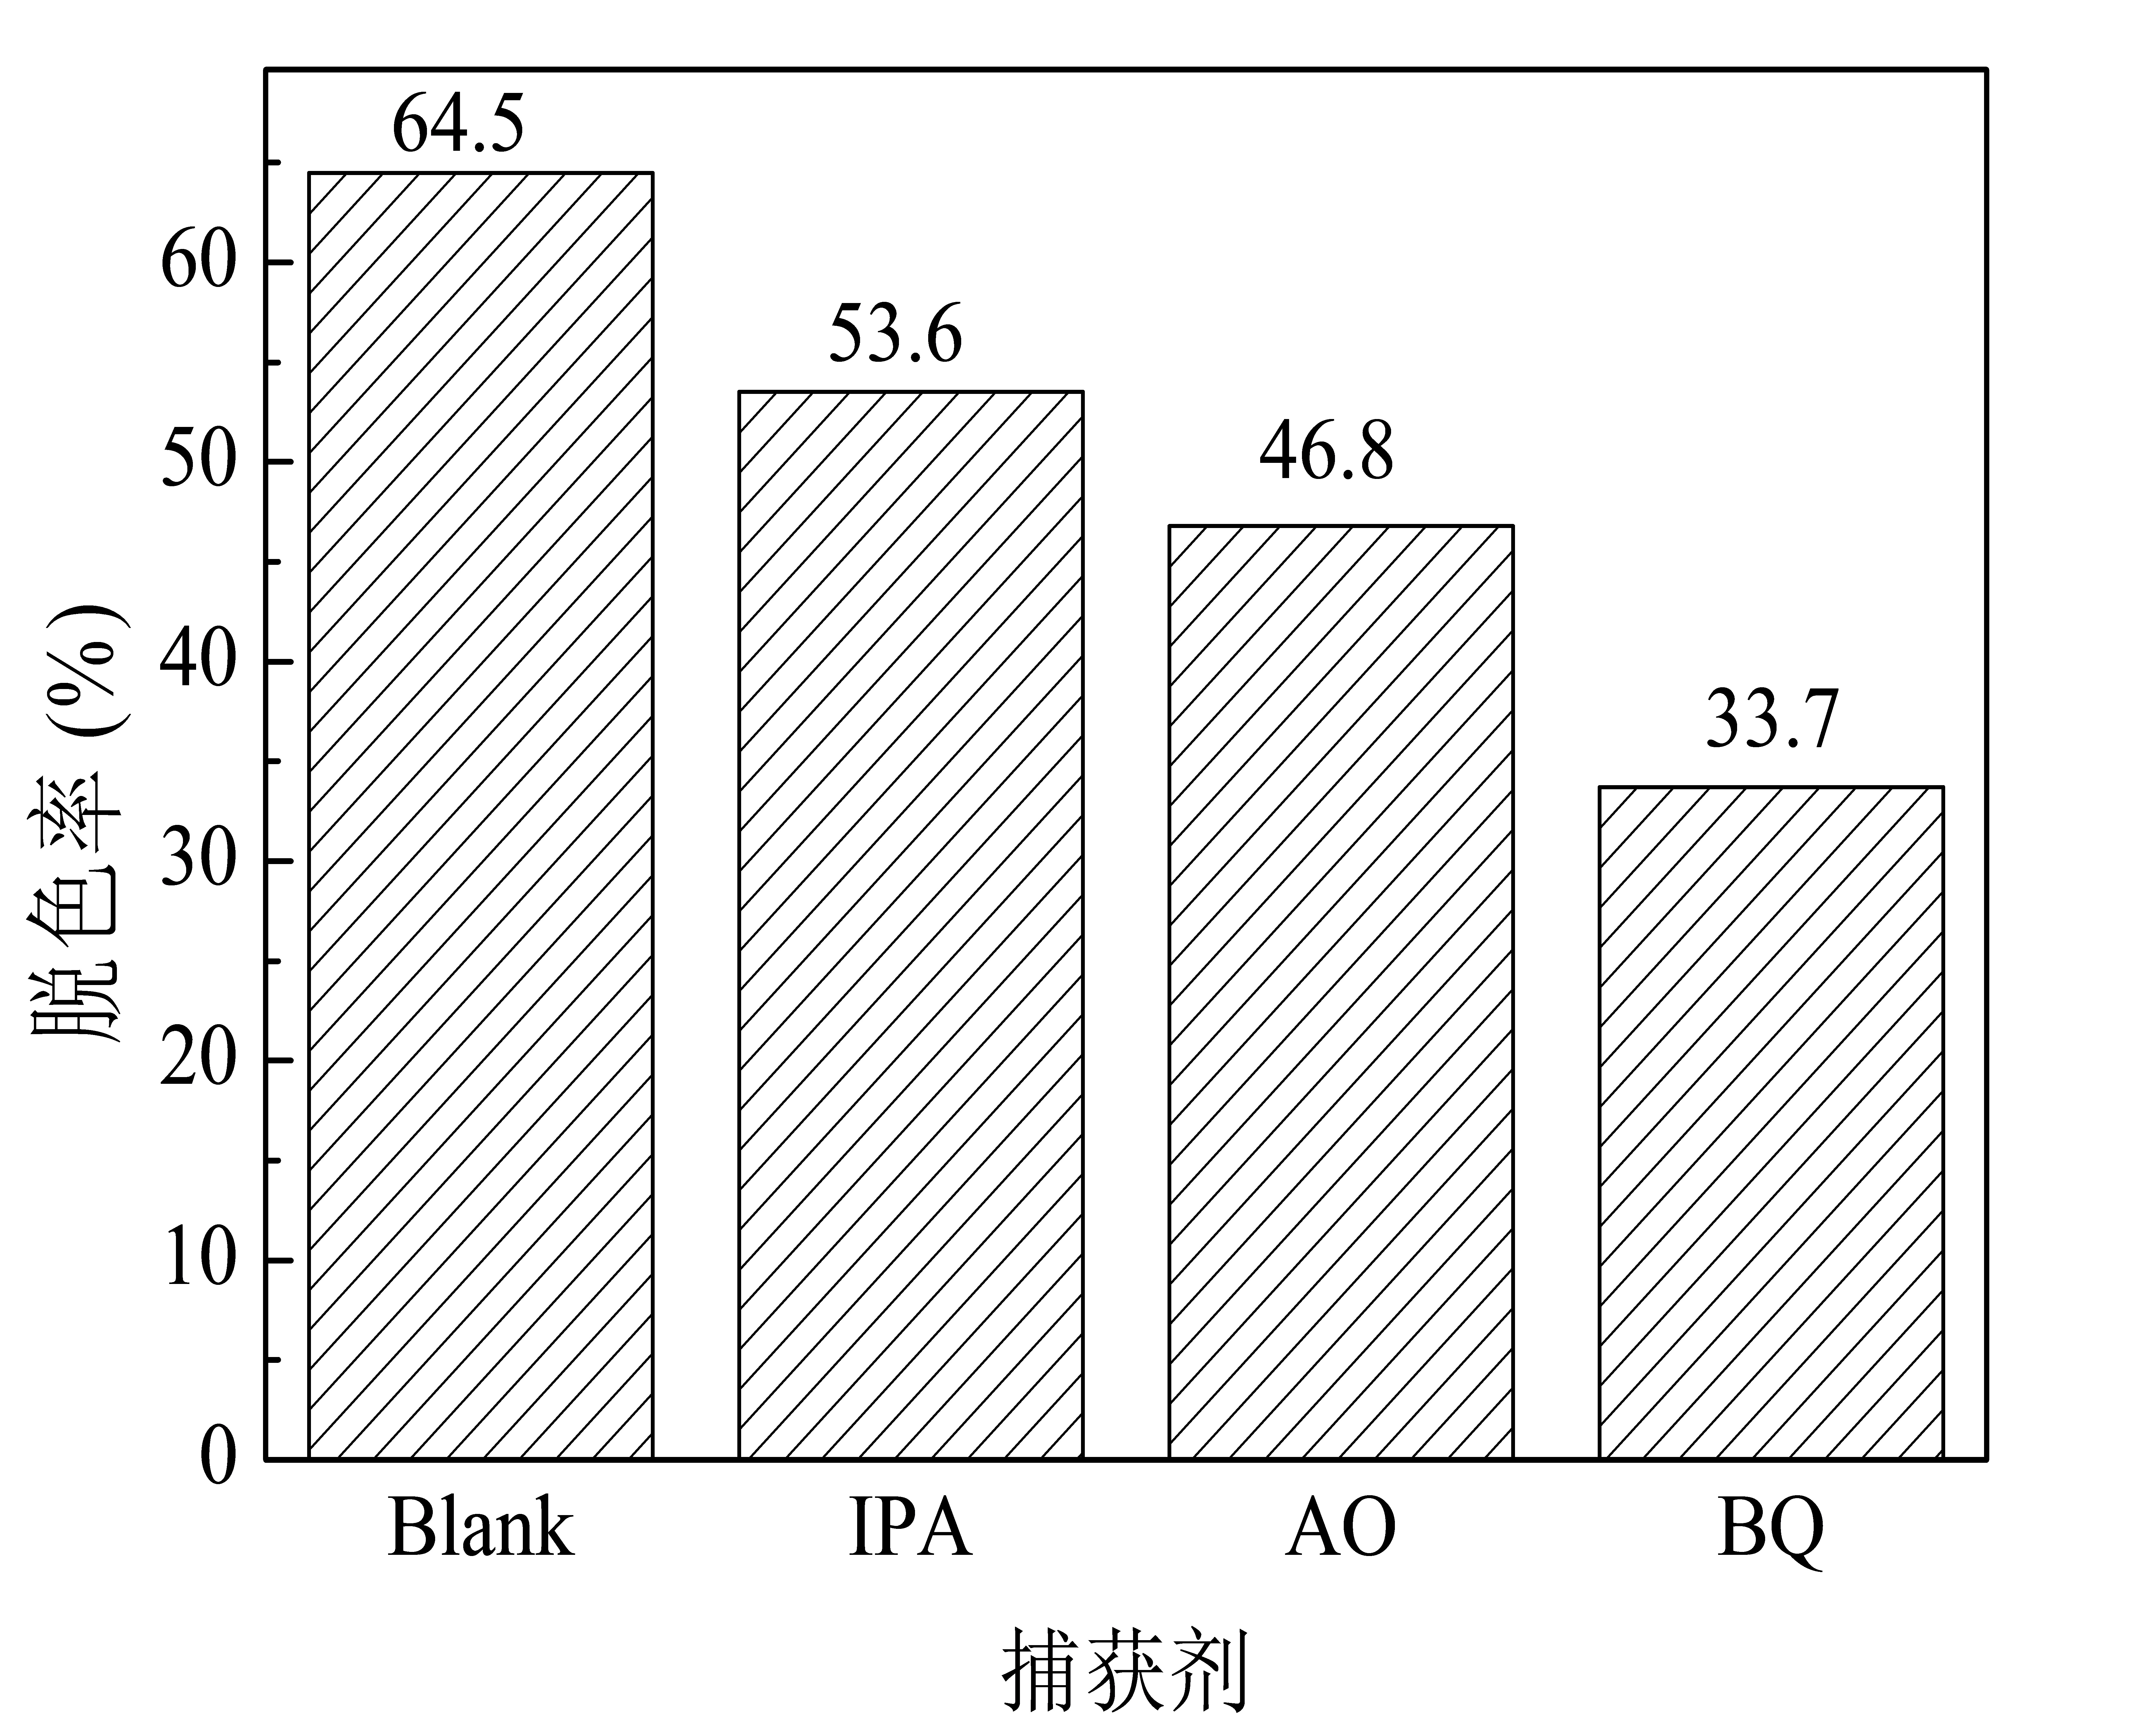
\includegraphics[width=\linewidth]{figures/三氧化二铁捕获剂.jpg} 
\end{block}
\column{0.5\textwidth}
\begin{block}{}
加入苯琨后甲基橙脱色率由 64.5\%急剧下降至 33.7\%,这表明•O$\mathbf{^{2-}} $ 是主要的活性自由基,加入异丙醇和草酸铵后甲基橙脱色率由 64.5\%分别下降至 46.8 和 53.6\%,这说明•OH 和 h+起次要作用。
\end{block}
\end{columns}
\end{frame}


\begin{frame}
\frametitle{\chemfig{\mathbf{Fe_2O_3/Bi_2O_3}}光催化剂的光催化活性}
\begin{block}{}
\centering
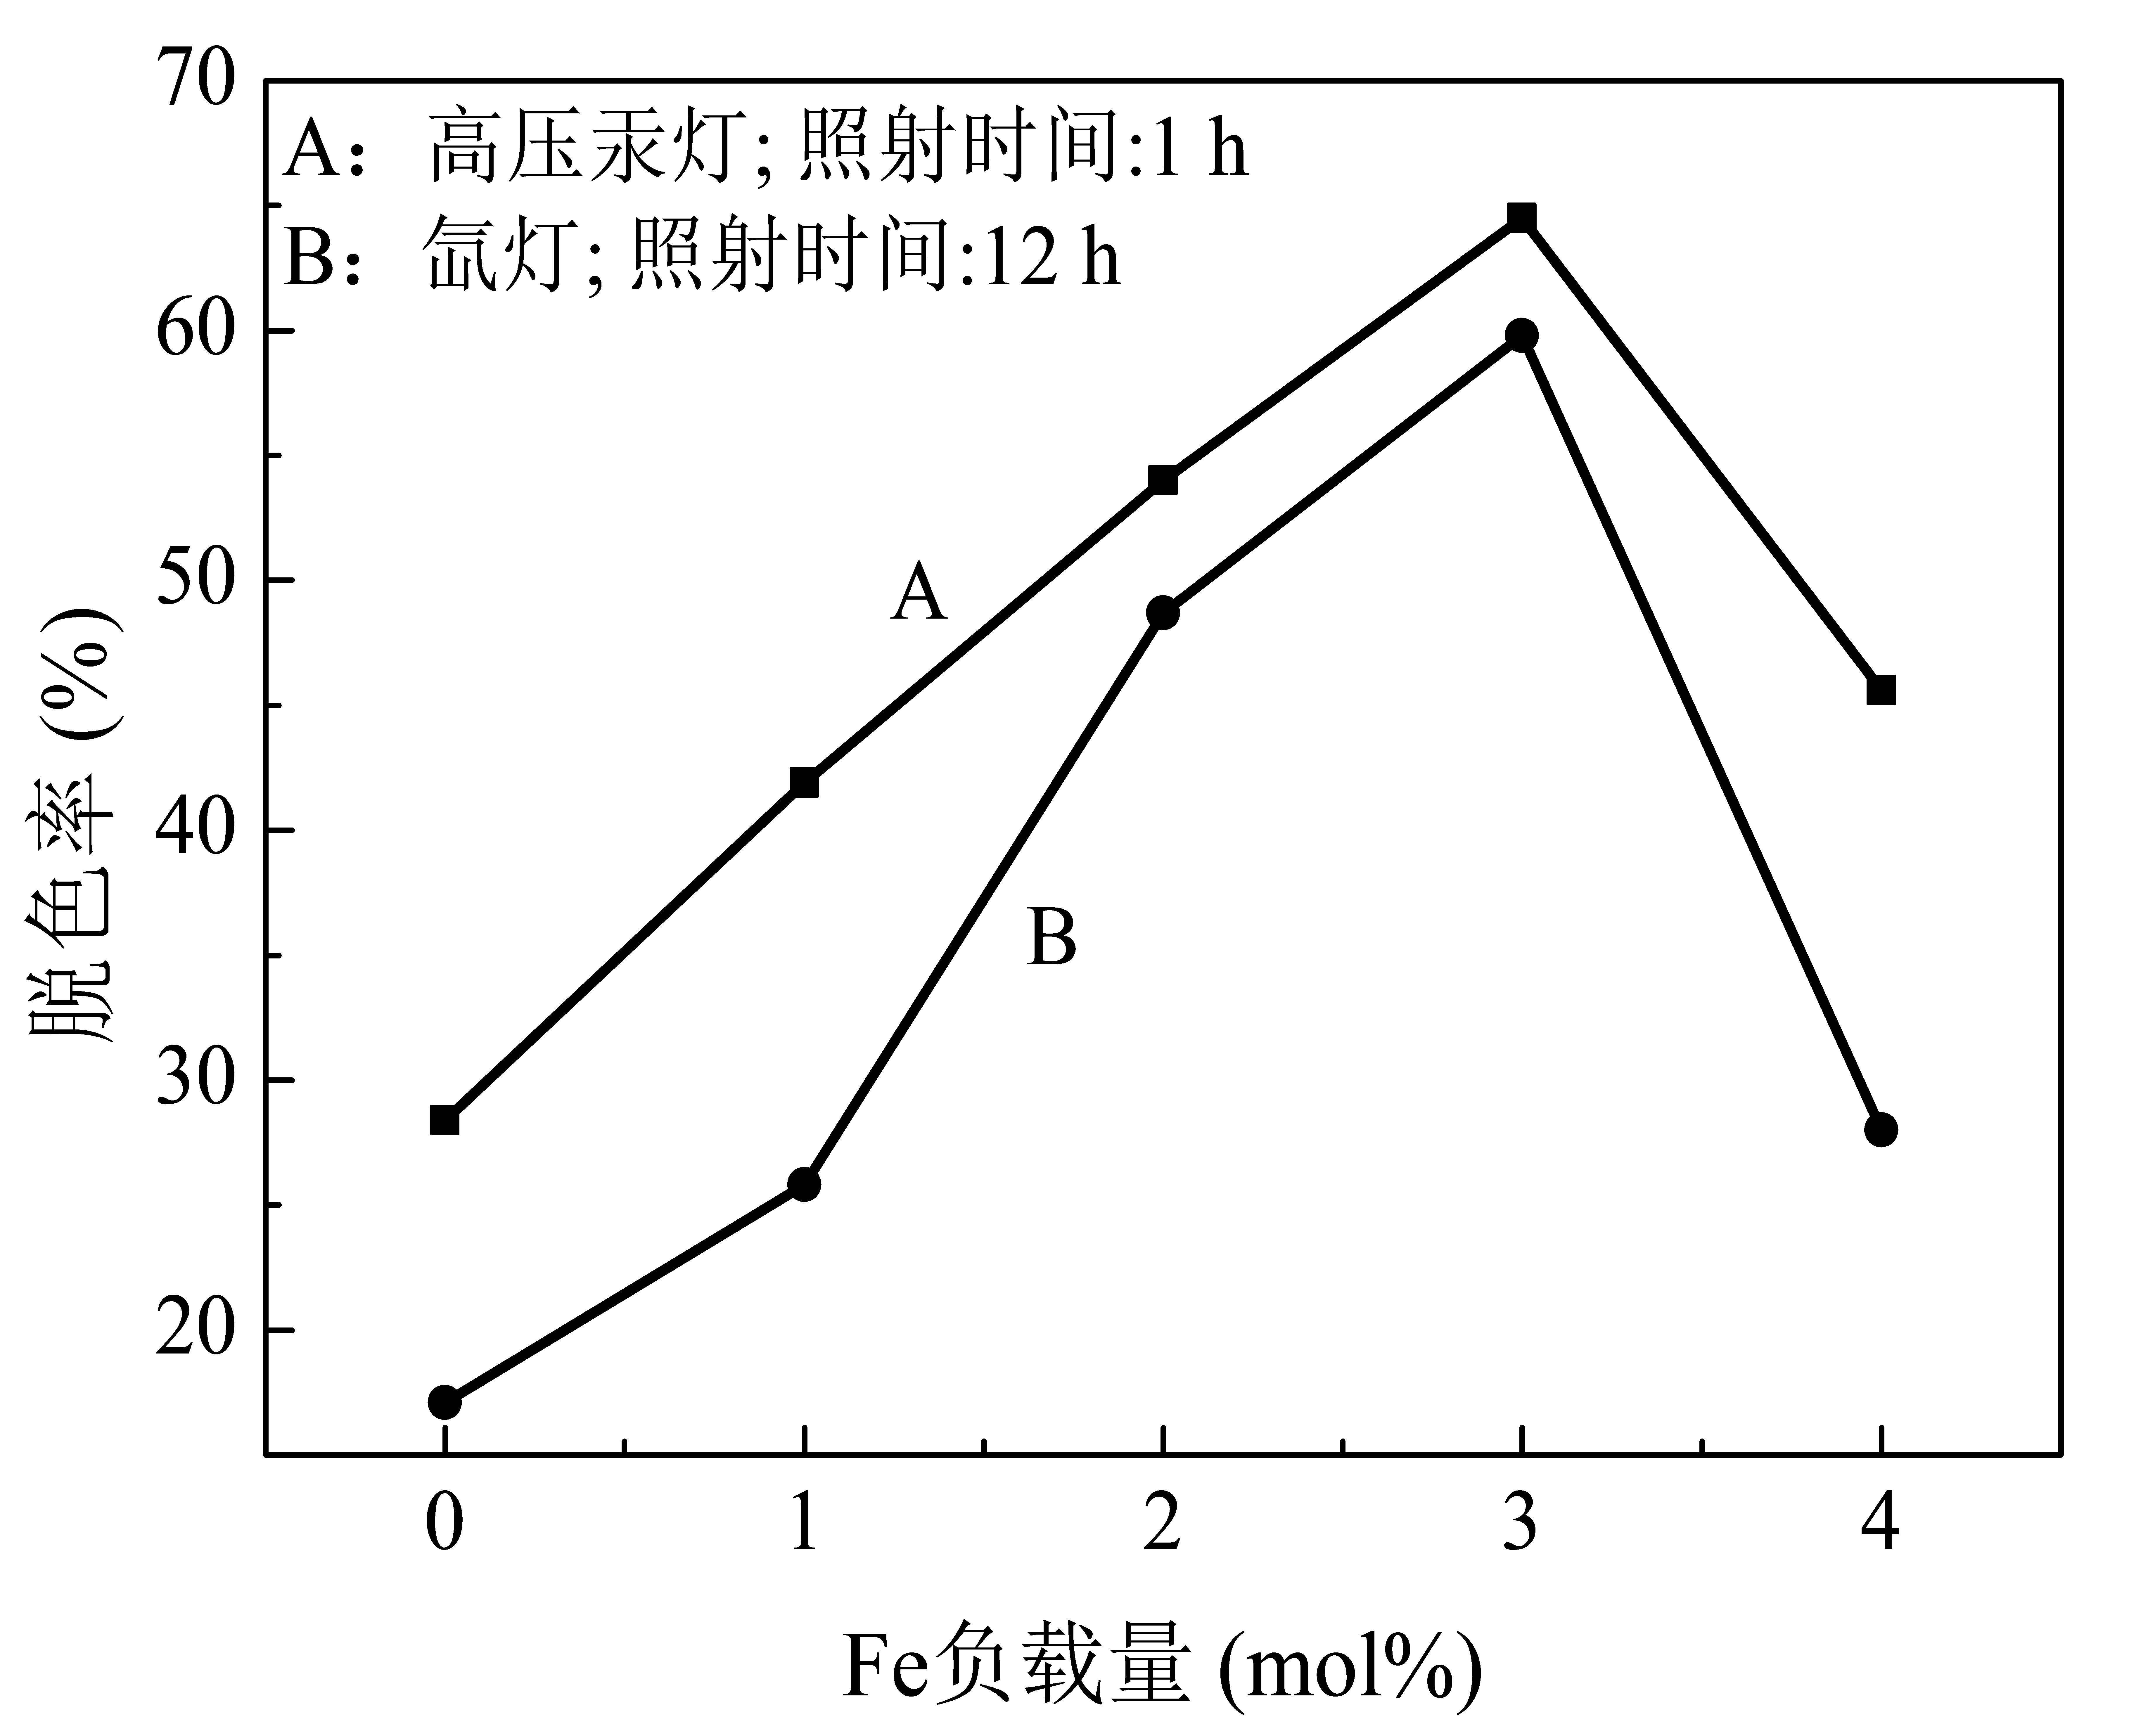
\includegraphics[width=0.8\textwidth]{figures/三氧化二铁脱色率一.jpg} 
\end{block}
\end{frame}


\begin{frame}
\frametitle{\chemfig{\mathbf{Fe_2O_3/Bi_2O_3}}光催化剂研究总结}
\begin{block}{}
\begin{itemize}
\item 在\chemfig{\mathbf{Bi_2O_3}}表面负载\chemfig{\mathbf{Fe_2O_3}}后表征结果显示形成了α-\chemfig{\mathbf{Fe_2O_3/Bi_2O_3}}异质结,部分\chemfig{\mathbf{Fe^{3+}}}离子进入\chemfig{\mathbf{Bi_2O_3}}晶格,引起特征衍射峰的位移,α-\chemfig{\mathbf{Fe_2O_3}}和 \chemfig{\mathbf{Bi_2O_3}}存在强的耦合作用,从而光生载流子分离效应增强,能带值降低,所制备异质结对甲基橙光催化活性得到显著提高,Fe/Bi原子比为3\%样品具有最好的太阳光和紫外光催化活性。
\end{itemize}
\end{block}
\end{frame}


\subsection{氧化镍}
\begin{frame}
\frametitle{\chemfig{\mathbf{NiO/Bi_2O_3}}光催化剂XRD图谱}
\begin{block}{}
\centering
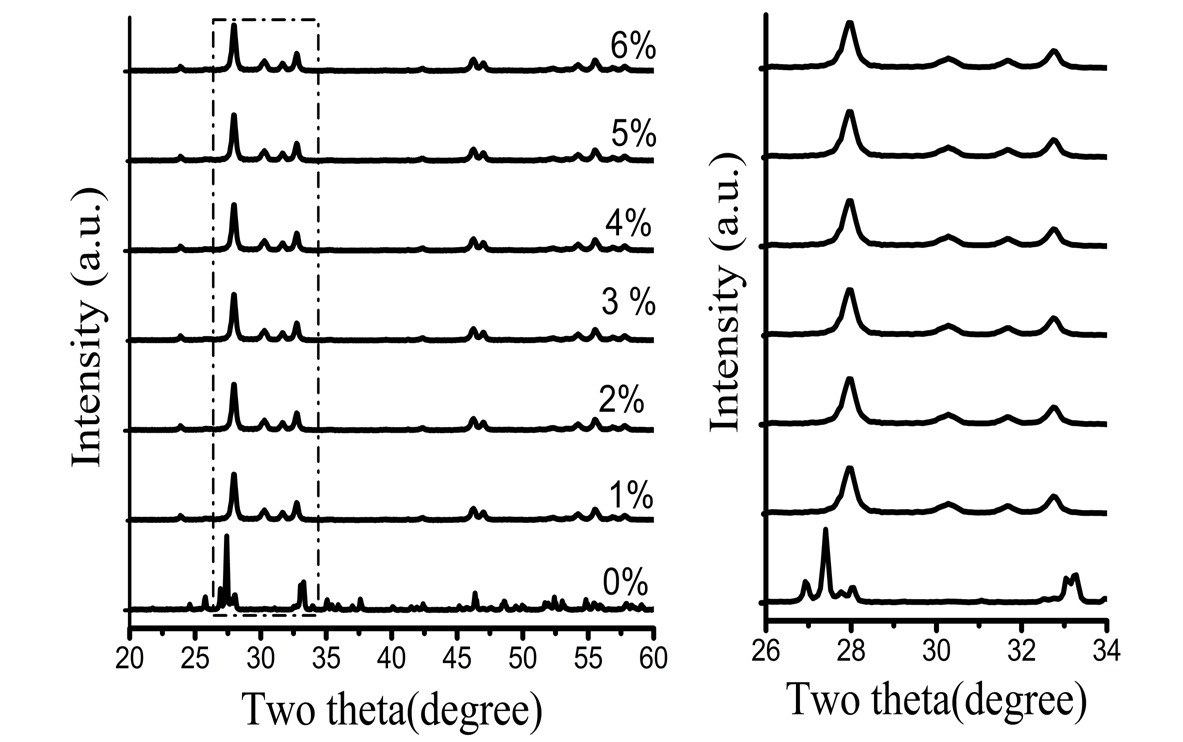
\includegraphics[width=0.9\linewidth]{figures/氧化镍XRD} 
\end{block}
\end{frame}

\begin{frame}
\frametitle{\chemfig{\mathbf{NiO/Bi_2O_3}}光催化剂比表面积}
\begin{block}{}
\centering
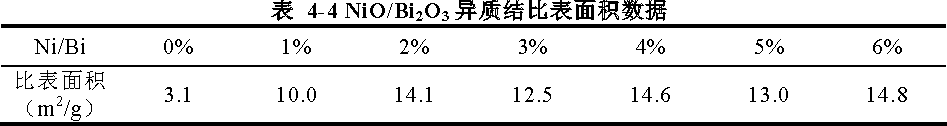
\includegraphics[width=\linewidth]{figures/氧化镍比表面积} 
\end{block}
\begin{block}{}
当\chemfig{\mathbf{Bi_2O_3}}与NiO形成异质结后,其比表面积显著增加。负载量超过2\%后,其比表面积变化较小,趋于稳定,这与 XRD 图谱中衍射峰宽化程度相一致。
\end{block}
\end{frame}


\begin{frame}
\frametitle{\chemfig{\mathbf{NiO/Bi_2O_3}}光催化剂UV-Vis图谱}
\begin{block}{}
\centering
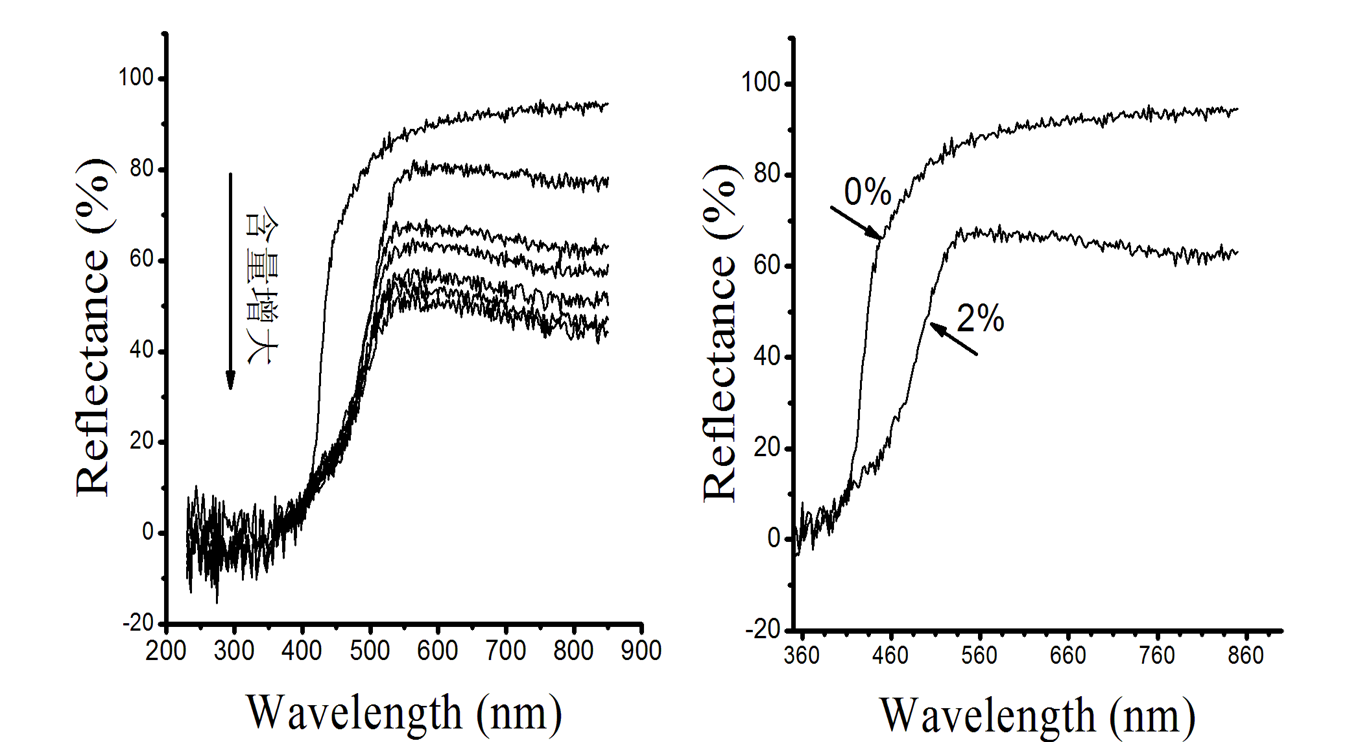
\includegraphics[width=\textwidth]{figures/氧化镍UV} 
\end{block}
\end{frame}


\begin{frame}
\frametitle{\chemfig{\mathbf{NiO/Bi_2O_3}}光催化剂的光催化活性}
\begin{block}{}
\centering
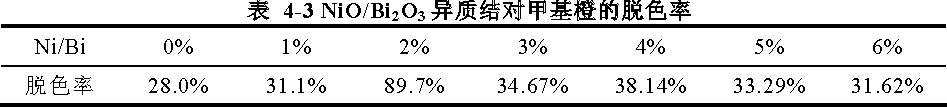
\includegraphics[width=\textwidth]{figures/氧化镍脱色率} 
\end{block}
\begin{block}{\chemfig{\mathbf{NiO/Bi_2O_3}}光催化剂研究总结}
在\chemfig{\mathbf{Bi_2O_3}}表面负载NiO后比表面增加,NiO和\chemfig{\mathbf{Bi_2O_3}}存在强的耦合作用,异质结在400到800 nm区域内对光有着更好的吸收,Ni/Bi原子比为2\%样品具有紫外光催化活性,光照1小时后2\%样品对甲基橙的脱色率较\chemfig{\mathbf{Bi_2O_3}}对甲基橙的脱色率提高了约4倍。
\end{block}
\end{frame}


\subsection{氧化锌}
\begin{frame}
\frametitle{\chemfig{\mathbf{ZnO/Bi_2O_3}}光催化剂XRD图谱}
\begin{block}{}
\centering
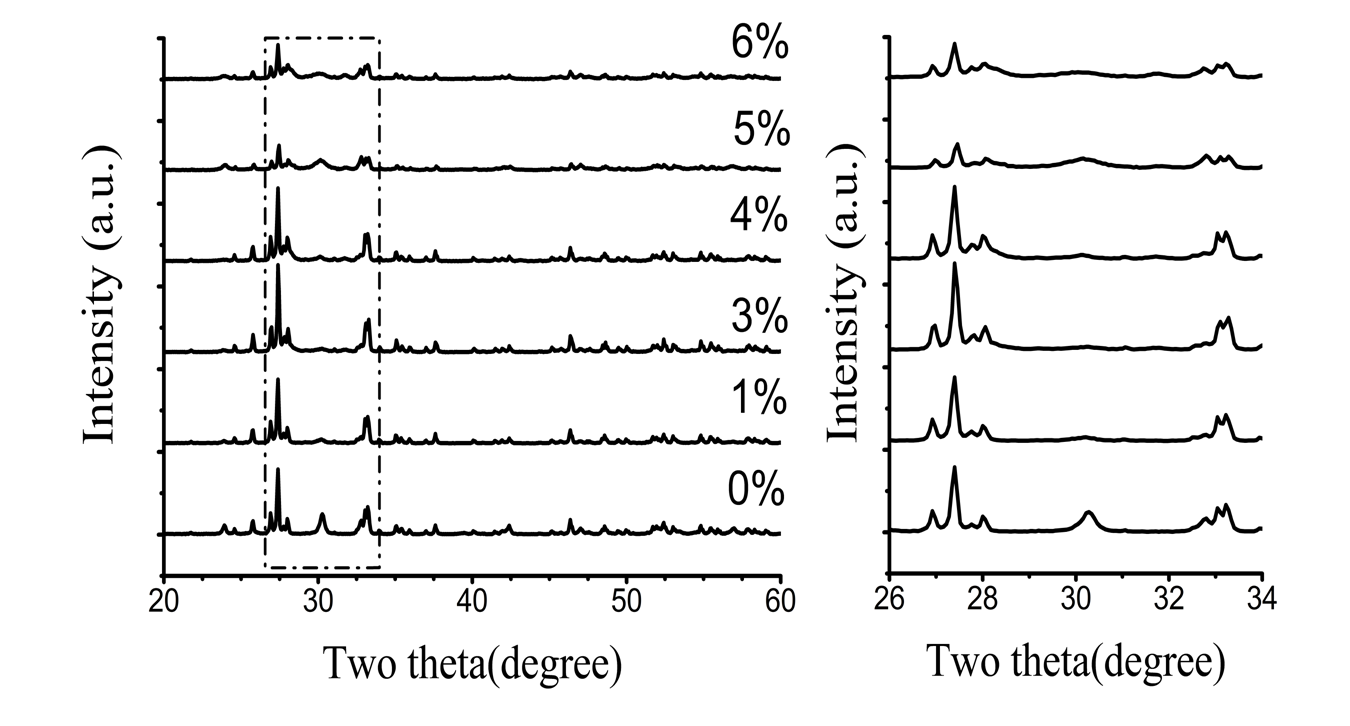
\includegraphics[width=\linewidth]{figures/氧化锌XRD} 
\end{block}
\end{frame}

\begin{frame}
\frametitle{\chemfig{\mathbf{ZnO/Bi_2O_3}}光催化剂比表面积}
\begin{block}{}
\centering
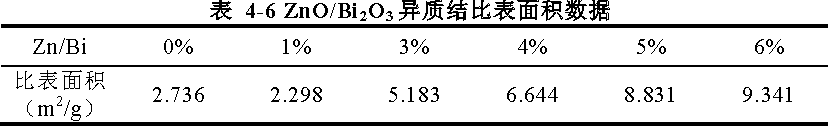
\includegraphics[width=\linewidth]{figures/氧化锌比表面积} 
\end{block}
\begin{block}{}
从表中可知,随着 ZnO含量的增多,异质结的比表面积发生了较大变化。当复合量为 6\%时,异质结比表
面积为\chemfig{\mathbf{Bi_2O_3}}的 3.5 倍。高的比表面有利于高催化活性的提高。
\end{block}
\end{frame}


\begin{frame}
\frametitle{\chemfig{\mathbf{ZnO/Bi_2O_3}}光催化剂UV-Vis图谱}
\begin{block}{}
\centering
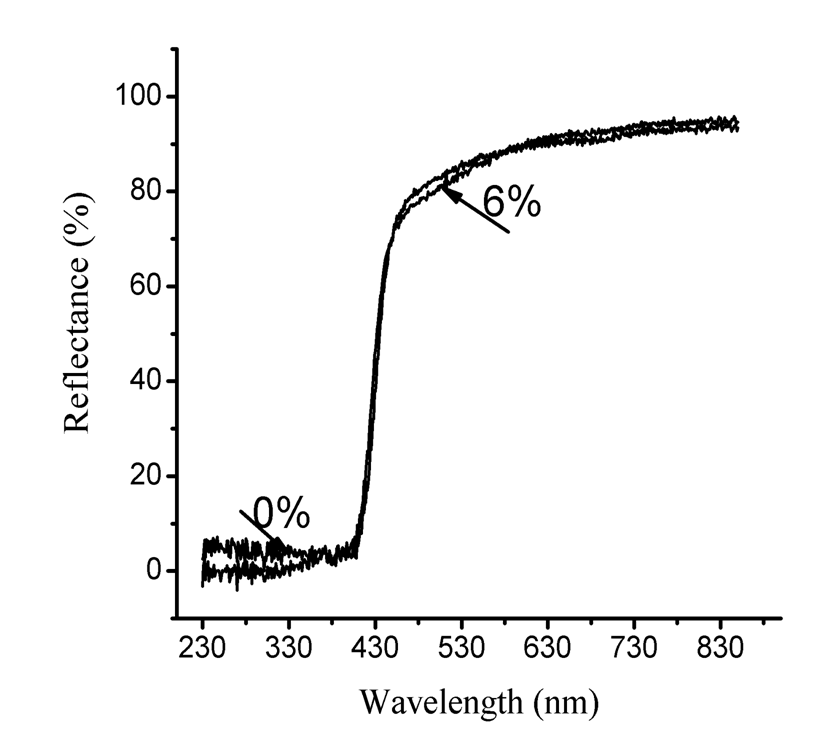
\includegraphics[width=0.68\textwidth]{figures/氧化锌UV} 
\end{block}
\end{frame}


\begin{frame}
\frametitle{\chemfig{\mathbf{ZnO/Bi_2O_3}}光催化剂的光催化活性}
\begin{block}{}
\centering
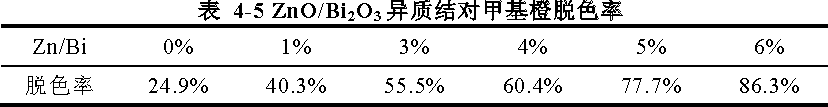
\includegraphics[width=\textwidth]{figures/氧化锌脱色率} 
\end{block}
\begin{block}{\chemfig{\mathbf{ZnO/Bi_2O_3}}光催化剂研究总结}
\chemfig{\mathbf{ZnO/Bi_2O_3}}异质结的比表面随着ZnO含量增加而逐渐增加,ZnO和\chemfig{\mathbf{Bi_2O_3}}存在强的耦合作用,光催化活性随ZnO含量增加而提高。
\end{block}
\end{frame}



\section{结语}
\subsection{光催化剂的应用前景}
\begin{frame}
\frametitle{光催化剂的应用前景}
\begin{block}{}
由于\chemfig{\mathbf{TiO_2}}既能够杀菌,又能够吸附灰尘,还能够光催化降解甲醛,含氮有害气体等等。因此目前将\chemfig{\mathbf{TiO_2}}用于室内空气净化是一个热门课题也是商业上的一个热点。前面谈到制约\chemfig{\mathbf{TiO_2}}应用的最大一点就是禁带能宽过大,而三氧化二铋的吸收谱带先天就比\chemfig{\mathbf{TiO_2}}要宽,如果三氧化二铋通过改性在稳定性和催化活性上进一步提
升,那么它的应用前景也是很广阔的
\end{block}
\end{frame}


\begin{frame}
\frametitle{可能存在的环境问题}
\begin{block}{}
在 2003 年全美化学年会上科学家们就提出金属、陶瓷、有机纳米材料可能有毒。后来科学家们也证实人的发病率和他们生活环境的空气颗粒浓度和颗粒尺寸大小密切相关,死亡率的增加是由那些剂量很低相对较小的颗粒物引起的 。Rahman 等用 20 nm 的超细\chemfig{\mathbf{TiO_2}}处理纤维细胞,发现经过处理后的细胞,细胞核核仁消失,细胞膜起泡,DNA 出现随机断裂,可见纳米\chemfig{\mathbf{TiO_2}}能够引起细胞凋亡。
\end{block}
\end{frame}

\begin{frame}
\frametitle{下一步的工作展望}
\begin{block}{}
本论文仍有许多不足之处,首先是对镨和钕掺杂\chemfig{\mathbf{Bi_2O_3}}形貌的控制、中间产物形式、高温转相和低温转相的行为,对镨和钕离子在\chemfig{\mathbf{Bi_2O_3}}晶格内的掺杂形式缺乏更为深入认识;对异质结表面电荷性质、密度认识不深入;对氧化铋降解反应后的性能和稳定性尚待进一步研究;其次是对甲基橙在\chemfig{\mathbf{Bi_2O_3}}基光催化剂表面光催化脱色降解产物表征不够。今后的研究目标是进一步深入探讨柠檬酸溶胶-凝胶法制备的纳米氧化铋过程规律,以及\chemfig{\mathbf{Bi_2O_3}}基光催化剂光催化降解有机污染物的详细过程规律,为其实际应用提供理论依据。
\end{block}
\end{frame}

\subsection{致谢}
\begin{frame}
\frametitle{致谢}
\begin{block}{}
本实验工作是在李建章教授的悉心指导下完成的,在此特向李建章老师致以诚挚的谢意!感谢李建章老师三年来对我的教诲与关怀,使我得以顺利完成学业。李建章老师正直的为人、踏实的作风与开拓的精神令我受益匪浅。

在这里,我还要感谢钟俊波、曾俊老师以及实验室的何锡阳老师、王涛老师,他们热情的关心和帮助,以及在研究过程中给提出的宝贵指导与建议,为我排除了工作中的许多困难。在此,我真诚地向他们表示感谢!

还要感谢本实验室的研究生和本科生对我的支持。他们是王绍华、黄春。

最后,我还要感谢在我身后默默支持我的家人!
\end{block}
\end{frame}

\end{document}
